\documentclass[twoside]{book}

% Packages required by doxygen
\usepackage{fixltx2e}
\usepackage{calc}
\usepackage{doxygen}
\usepackage[export]{adjustbox} % also loads graphicx
\usepackage{graphicx}
\usepackage[utf8]{inputenc}
\usepackage{makeidx}
\usepackage{multicol}
\usepackage{multirow}
\PassOptionsToPackage{warn}{textcomp}
\usepackage{textcomp}
\usepackage[nointegrals]{wasysym}
\usepackage[table]{xcolor}

% Font selection
\usepackage[T1]{fontenc}
\usepackage[scaled=.90]{helvet}
\usepackage{courier}
\usepackage{amssymb}
\usepackage{sectsty}
\renewcommand{\familydefault}{\sfdefault}
\allsectionsfont{%
  \fontseries{bc}\selectfont%
  \color{darkgray}%
}
\renewcommand{\DoxyLabelFont}{%
  \fontseries{bc}\selectfont%
  \color{darkgray}%
}
\newcommand{\+}{\discretionary{\mbox{\scriptsize$\hookleftarrow$}}{}{}}

% Page & text layout
\usepackage{geometry}
\geometry{%
  a4paper,%
  top=2.5cm,%
  bottom=2.5cm,%
  left=2.5cm,%
  right=2.5cm%
}
\tolerance=750
\hfuzz=15pt
\hbadness=750
\setlength{\emergencystretch}{15pt}
\setlength{\parindent}{0cm}
\setlength{\parskip}{0.2cm}
\makeatletter
\renewcommand{\paragraph}{%
  \@startsection{paragraph}{4}{0ex}{-1.0ex}{1.0ex}{%
    \normalfont\normalsize\bfseries\SS@parafont%
  }%
}
\renewcommand{\subparagraph}{%
  \@startsection{subparagraph}{5}{0ex}{-1.0ex}{1.0ex}{%
    \normalfont\normalsize\bfseries\SS@subparafont%
  }%
}
\makeatother

% Headers & footers
\usepackage{fancyhdr}
\pagestyle{fancyplain}
\fancyhead[LE]{\fancyplain{}{\bfseries\thepage}}
\fancyhead[CE]{\fancyplain{}{}}
\fancyhead[RE]{\fancyplain{}{\bfseries\leftmark}}
\fancyhead[LO]{\fancyplain{}{\bfseries\rightmark}}
\fancyhead[CO]{\fancyplain{}{}}
\fancyhead[RO]{\fancyplain{}{\bfseries\thepage}}
\fancyfoot[LE]{\fancyplain{}{}}
\fancyfoot[CE]{\fancyplain{}{}}
\fancyfoot[RE]{\fancyplain{}{\bfseries\scriptsize Generated on Sun Feb 28 2016 22\+:27\+:10 for A\+B\+M\+Solar by Doxygen }}
\fancyfoot[LO]{\fancyplain{}{\bfseries\scriptsize Generated on Sun Feb 28 2016 22\+:27\+:10 for A\+B\+M\+Solar by Doxygen }}
\fancyfoot[CO]{\fancyplain{}{}}
\fancyfoot[RO]{\fancyplain{}{}}
\renewcommand{\footrulewidth}{0.4pt}
\renewcommand{\chaptermark}[1]{%
  \markboth{#1}{}%
}
\renewcommand{\sectionmark}[1]{%
  \markright{\thesection\ #1}%
}

% Indices & bibliography
\usepackage{natbib}
\usepackage[titles]{tocloft}
\setcounter{tocdepth}{3}
\setcounter{secnumdepth}{5}
\makeindex

% Hyperlinks (required, but should be loaded last)
\usepackage{ifpdf}
\ifpdf
  \usepackage[pdftex,pagebackref=true]{hyperref}
\else
  \usepackage[ps2pdf,pagebackref=true]{hyperref}
\fi
\hypersetup{%
  colorlinks=true,%
  linkcolor=blue,%
  citecolor=blue,%
  unicode%
}

% Custom commands
\newcommand{\clearemptydoublepage}{%
  \newpage{\pagestyle{empty}\cleardoublepage}%
}


%===== C O N T E N T S =====

\begin{document}

% Titlepage & ToC
\hypersetup{pageanchor=false,
             bookmarks=true,
             bookmarksnumbered=true,
             pdfencoding=unicode
            }
\pagenumbering{roman}
\begin{titlepage}
\vspace*{7cm}
\begin{center}%
{\Large A\+B\+M\+Solar }\\
\vspace*{1cm}
{\large Generated by Doxygen 1.8.9.1}\\
\vspace*{0.5cm}
{\small Sun Feb 28 2016 22:27:10}\\
\end{center}
\end{titlepage}
\clearemptydoublepage
\tableofcontents
\clearemptydoublepage
\pagenumbering{arabic}
\hypersetup{pageanchor=true}

%--- Begin generated contents ---
\chapter{Dev\+Stage1}
\label{_dev_stage1}
\hypertarget{_dev_stage1}{}

\begin{DoxyRefList}
\item[\label{_dev_stage1__DevStage1000001}%
\hypertarget{_dev_stage1__DevStage1000001}{}%
Class \hyperlink{class_marketing_inst}{Marketing\+Inst} ]Will inherit from Insititute
\end{DoxyRefList}
\chapter{Dev\+Stage2}
\label{_dev_stage2}
\hypertarget{_dev_stage2}{}

\begin{DoxyRefList}
\item[\label{_dev_stage2__DevStage2000026}%
\hypertarget{_dev_stage2__DevStage2000026}{}%
Member \hyperlink{namespaceserialize_aa5ee0bad0c960a3f06430066217d8c12}{serialize\+:\+:solve\+\_\+str\+\_\+formula} (const std\+::string \&formula\+\_\+, I\+Random \&rand\+\_\+)]change to better Truncated generation, now is simple rejection algorithm  
\item[\label{_dev_stage2__DevStage2000025}%
\hypertarget{_dev_stage2__DevStage2000025}{}%
Member \hyperlink{namespacesolar__core_aa1147341e5ef7a40d68d1bd68e149362}{solar\+\_\+core\+:\+:E\+Param\+Types} ]think about splitting enum into multiple enums 
\item[\label{_dev_stage2__DevStage2000001}%
\hypertarget{_dev_stage2__DevStage2000001}{}%
Member \hyperlink{classsolar__core_1_1_g_a624adac31ade604e0335717bad4fc9cd}{solar\+\_\+core\+:\+:G\+:\+:G} (const Property\+Tree \&pt\+\_\+, \hyperlink{classsolar__core_1_1_w}{W} $\ast$w\+\_\+)]move to \hyperlink{classsolar__core_1_1_w}{W} to speed up, but test before that  
\item[\label{_dev_stage2__DevStage2000002}%
\hypertarget{_dev_stage2__DevStage2000002}{}%
Member \hyperlink{classsolar__core_1_1_g_a33472d3b331a303ec8a9b61e2da163d3}{solar\+\_\+core\+:\+:G\+:\+:schedule\+\_\+visits} ]think about it, not every jurisdiction will need it  
\item[\label{_dev_stage2__DevStage2000007}%
\hypertarget{_dev_stage2__DevStage2000007}{}%
Class \hyperlink{classsolar__core_1_1_household}{solar\+\_\+core\+:\+:Household} ]might change from actually assigning house to assigning house type (memory considerations) 
\item[\label{_dev_stage2__DevStage2000004}%
\hypertarget{_dev_stage2__DevStage2000004}{}%
Member \hyperlink{classsolar__core_1_1_household_a165b7c64c72e5ed4ea08307e32082517}{solar\+\_\+core\+:\+:Household\+:\+:ac\+\_\+inf\+\_\+quoting\+\_\+sei} ()]think about moving difference to the virtual call. For now it is explicit, as it is assumed that agents themselves realize that it will be online vs offline quote  
\item[\label{_dev_stage2__DevStage2000006}%
\hypertarget{_dev_stage2__DevStage2000006}{}%
Member \hyperlink{classsolar__core_1_1_household_a1e7d20a60dc42b8d09a8d23a4cdb26a6}{solar\+\_\+core\+:\+:Household\+:\+:act\+\_\+tick} ()]generally actions in a tick depend on the state of an agent, either it is choosing installer or waiting for the project to finish. Might have a call back to w that will indicate that this agent has changed state. In this case w will have multiple lists of agents in different states and would call appropriate function. Or might do it internally where new state will dictate behavior in the tick. Generally have both -\/ agent is broadcasting changed state and behaves differently depending on the state.  
\item[\label{_dev_stage2__DevStage2000005}%
\hypertarget{_dev_stage2__DevStage2000005}{}%
Member \hyperlink{classsolar__core_1_1_household_aaa1f1e52009d8aef32d3c5a9367b93b7}{solar\+\_\+core\+:\+:Household\+:\+:dec\+\_\+evaluate\+\_\+designs} ()]may go back and forth over the design 
\item[\label{_dev_stage2__DevStage2000009}%
\hypertarget{_dev_stage2__DevStage2000009}{}%
Member \hyperlink{classsolar__core_1_1_household_aa63241ca3fcc1f2374d10b5c7f44124a}{solar\+\_\+core\+:\+:Household\+:\+:dec\+\_\+project\+\_\+reroof} (std\+::shared\+\_\+ptr$<$ P\+V\+Project $>$ project)]need to ask H\+H how they decide to reroof  
\item[\label{_dev_stage2__DevStage2000003}%
\hypertarget{_dev_stage2__DevStage2000003}{}%
Member \hyperlink{classsolar__core_1_1_household_ac9d26af7b52f0cdc357fc5dca4b86ad9}{solar\+\_\+core\+:\+:Household\+:\+:get\+\_\+inf} (std\+::shared\+\_\+ptr$<$ Mes\+Marketing\+S\+E\+I $>$ mes\+\_\+) override]might be add saving of the time of the marketing message, in this case it will be saved in the form of transformed marketing messages because original message will time stamped at the moment of creation (almost at the beginning of the simulation)  
\item[\label{_dev_stage2__DevStage2000011}%
\hypertarget{_dev_stage2__DevStage2000011}{}%
Member \hyperlink{classsolar__core_1_1_household_a1104d8264fe733937e1fd2e9ad0f8fc1}{solar\+\_\+core\+:\+:Household\+:\+:house} ]think about decreasing size for this field, use uint64\+\_\+t or smaller for it  
\item[\label{_dev_stage2__DevStage2000008}%
\hypertarget{_dev_stage2__DevStage2000008}{}%
Member \hyperlink{classsolar__core_1_1_household_a5f84bf614d0ec70abf9597ec97e07b1a}{solar\+\_\+core\+:\+:Household\+:\+:Household} (Property\+Tree \&pt\+\_\+, \hyperlink{classsolar__core_1_1_w}{W} $\ast$w\+\_\+)]need destructor, copy constructor, copy assignment operator, move constructor, move assignment operator 
\item[\label{_dev_stage2__DevStage2000010}%
\hypertarget{_dev_stage2__DevStage2000010}{}%
Member \hyperlink{classsolar__core_1_1_household_a1ba6b7af82982096e05d99a70a2647eb}{solar\+\_\+core\+:\+:Household\+:\+:location\+\_\+y} ]think about decreasing size for this field, use uint64\+\_\+t or smaller for it  
\item[\label{_dev_stage2__DevStage2000012}%
\hypertarget{_dev_stage2__DevStage2000012}{}%
Member \hyperlink{classsolar__core_1_1_household_a297842358a2d79db160566106972bc0d}{solar\+\_\+core\+:\+:Household\+:\+:preliminary\+\_\+quotes} ]think about replacing raw pointer with. 

choose between week\+\_\+ptr and shared\+\_\+ptr need to think about ownership in time and time of destruction for these messages.  
\item[\label{_dev_stage2__DevStage2000024}%
\hypertarget{_dev_stage2__DevStage2000024}{}%
Class \hyperlink{classsolar__core_1_1_mes_marketing_s_e_i_online_quote}{solar\+\_\+core\+:\+:Mes\+Marketing\+S\+E\+I\+Online\+Quote} ]think, for now this message is used in the first stage of quoting. If decide to use in the next stage might have to add field to indicate from what stage of quoting this message is. Alternative is to have separate classes for different quotes from different stages. Actually like it more. Need to have base message class to avoid multiple containers for them. But at the same time it might be actually more efficient to have multiple containers for different stages of quoting. It will make search and compare much quicker... 
\item[\label{_dev_stage2__DevStage2000016}%
\hypertarget{_dev_stage2__DevStage2000016}{}%
Class \hyperlink{classsolar__core_1_1_s_e_i}{solar\+\_\+core\+:\+:S\+E\+I} ]might add timer to model that giving estimate might take time. Also might have queue and maximum capacity, thus receiving quote in place might actually take some time before requesting online visit and actually performing this visit 
\item[\label{_dev_stage2__DevStage2000015}%
\hypertarget{_dev_stage2__DevStage2000015}{}%
Member \hyperlink{classsolar__core_1_1_s_e_i_ab84401c625f5c459accf430535e4a06d}{solar\+\_\+core\+:\+:S\+E\+I\+:\+:ac\+\_\+estimate\+\_\+savings} (\hyperlink{classsolar__core_1_1_p_v_design}{P\+V\+Design} \&design, std\+::shared\+\_\+ptr$<$ P\+V\+Project $>$ project\+\_\+)]\+: calculate P\+P\+A \+: calculate lease  
\item[\label{_dev_stage2__DevStage2000017}%
\hypertarget{_dev_stage2__DevStage2000017}{}%
Member \hyperlink{classsolar__core_1_1_s_e_i_ab0bd6ae650afc15fe71ce545373ab16e}{solar\+\_\+core\+:\+:S\+E\+I\+:\+:act\+\_\+tick} ()]might think about checking for the type of the tick in \hyperlink{classsolar__core_1_1_w}{W} and call proper sub tick method from there, will save on multiple boll checks, even of they are cheap.  
\item[\label{_dev_stage2__DevStage2000014}%
\hypertarget{_dev_stage2__DevStage2000014}{}%
Member \hyperlink{classsolar__core_1_1_s_e_i_a807561ad055ddc0df91b80ba406ee6df}{solar\+\_\+core\+:\+:S\+E\+I\+:\+:form\+\_\+design} (std\+::shared\+\_\+ptr$<$ P\+V\+Project $>$ project\+\_\+)]bootstrap here for different savings dynamics depending on parameters  
\item[\label{_dev_stage2__DevStage2000020}%
\hypertarget{_dev_stage2__DevStage2000020}{}%
Member \hyperlink{classsolar__core_1_1_s_e_i_ad532ca9d30d5988e051b75e33ce6c241}{solar\+\_\+core\+:\+:S\+E\+I\+:\+:form\+\_\+online\+\_\+quote} (std\+::shared\+\_\+ptr$<$ P\+V\+Project $>$ project\+\_\+)]think about transforming this call into interface based one, with agent\+\_\+in replaced by interface and it being virtual method from the general interface. But virtual call might be more costly and unnecessary in this case, as structure of who will be requesting quotes does not change.  
\item[\label{_dev_stage2__DevStage2000018}%
\hypertarget{_dev_stage2__DevStage2000018}{}%
Member \hyperlink{classsolar__core_1_1_s_e_i_a5fc331197d08788392c3af1903f25763}{solar\+\_\+core\+:\+:S\+E\+I\+:\+:location\+\_\+y} ]think about decreasing size for this field, use uint64\+\_\+t or smaller for it  
\item[\label{_dev_stage2__DevStage2000019}%
\hypertarget{_dev_stage2__DevStage2000019}{}%
Member \hyperlink{classsolar__core_1_1_s_e_i_a41711b0f344d6f29ea48dbcdb08b9c4e}{solar\+\_\+core\+:\+:S\+E\+I\+:\+:project\+\_\+states\+\_\+to\+\_\+delete} ]think about decreasing size for this field, use uint64\+\_\+t or smaller for it  
\item[\label{_dev_stage2__DevStage2000013}%
\hypertarget{_dev_stage2__DevStage2000013}{}%
Member \hyperlink{classsolar__core_1_1_s_e_i_af885d50c89decf5b6ff208c24cedd82b}{solar\+\_\+core\+:\+:S\+E\+I\+:\+:S\+E\+I} (const Property\+Tree \&pt\+\_\+, \hyperlink{classsolar__core_1_1_w}{W} $\ast$w\+\_\+)]move to \hyperlink{classsolar__core_1_1_w}{W} to speed up, but test before that  
\item[\label{_dev_stage2__DevStage2000022}%
\hypertarget{_dev_stage2__DevStage2000022}{}%
Class \hyperlink{classsolar__core_1_1_s_e_m}{solar\+\_\+core\+:\+:S\+E\+M} ]add market for solar panels and price feedback  
\item[\label{_dev_stage2__DevStage2000021}%
\hypertarget{_dev_stage2__DevStage2000021}{}%
Member \hyperlink{classsolar__core_1_1_s_e_m_a60d13fcadec26853d8461d32eefb97da}{solar\+\_\+core\+:\+:S\+E\+M\+:\+:S\+E\+M} (const Property\+Tree \&pt\+\_\+, \hyperlink{classsolar__core_1_1_w}{W} $\ast$w\+\_\+)]move to \hyperlink{classsolar__core_1_1_w}{W} to speed up, but test before that  
\item[\label{_dev_stage2__DevStage2000023}%
\hypertarget{_dev_stage2__DevStage2000023}{}%
Member \hyperlink{classsolar__core_1_1_utility_aa52a4877b6281d4ffa8f003b831e802c}{solar\+\_\+core\+:\+:Utility\+:\+:Utility} (const Property\+Tree \&pt\+\_\+, \hyperlink{classsolar__core_1_1_w}{W} $\ast$w\+\_\+)]move to \hyperlink{classsolar__core_1_1_w}{W} to speed up, but test before that  
\item[\label{_dev_stage2__DevStage2000029}%
\hypertarget{_dev_stage2__DevStage2000029}{}%
Member \hyperlink{classsolar__core_1_1_w_a1d35d6501eef6d673bd2b28e2c1724c4}{solar\+\_\+core\+:\+:W\+:\+:interconnected\+\_\+projects} ]think here, might change to weak\+\_\+ptr, but will pay the cost of checking each time if it is still alive  
\item[\label{_dev_stage2__DevStage2000028}%
\hypertarget{_dev_stage2__DevStage2000028}{}%
Member \hyperlink{classsolar__core_1_1_w_a969ad4de57020878a91873868c9bdb45}{solar\+\_\+core\+:\+:W\+:\+:W} (std\+::string path\+\_\+, \hyperlink{classsolar__core_1_1_helper_w}{Helper\+W} $\ast$w\+\_\+, std\+::string mode\+\_\+=\char`\"{}\+N\+E\+W\char`\"{})]\+: serialization\+: choose custom/binary/to database. For now think that cereal will be emough, with saving to .json. All agents of the same type will be saved in the same file. Loading also from .json with simple structure.

each sem will pick initial templates by name? -\/ could make it base creation mode 

each sem will pick initial templates by name? -\/ could make it base creation mode 
\end{DoxyRefList}
\chapter{Namespace Index}
\section{Namespace List}
Here is a list of all namespaces with brief descriptions\+:\begin{DoxyCompactList}
\item\contentsline{section}{\hyperlink{namespaceserialize}{serialize} }{\pageref{namespaceserialize}}{}
\item\contentsline{section}{\hyperlink{namespacesolar__core}{solar\+\_\+core} }{\pageref{namespacesolar__core}}{}
\item\contentsline{section}{\hyperlink{namespacesolar__core_1_1constants}{solar\+\_\+core\+::constants} }{\pageref{namespacesolar__core_1_1constants}}{}
\end{DoxyCompactList}

\chapter{Class Index}
\section{Class List}
Here are the classes, structs, unions and interfaces with brief descriptions\+:\begin{DoxyCompactList}
\item\contentsline{section}{\hyperlink{class_house}{House} }{\pageref{class_house}}{}
\item\contentsline{section}{\hyperlink{classsolar__core_1_1_household}{solar\+\_\+core\+::\+Household} }{\pageref{classsolar__core_1_1_household}}{}
\item\contentsline{section}{\hyperlink{class_marketing_inst}{Marketing\+Inst} }{\pageref{class_marketing_inst}}{}
\item\contentsline{section}{\hyperlink{classsolar__core_1_1_s_e_i}{solar\+\_\+core\+::\+S\+E\+I} }{\pageref{classsolar__core_1_1_s_e_i}}{}
\item\contentsline{section}{\hyperlink{class_tile}{Tile} }{\pageref{class_tile}}{}
\item\contentsline{section}{\hyperlink{classsolar__core_1_1_w}{solar\+\_\+core\+::\+W} }{\pageref{classsolar__core_1_1_w}}{}
\item\contentsline{section}{\hyperlink{class_world_map}{World\+Map} }{\pageref{class_world_map}}{}
\end{DoxyCompactList}

\chapter{File Index}
\section{File List}
Here is a list of all files with brief descriptions\+:\begin{DoxyCompactList}
\item\contentsline{section}{/\+Users/wilfeli/\+Dropbox/\+A\+B\+M/\+Solar\+Panels/\+A\+B\+M\+I\+R\+I\+S\+Lab/\+Source/\+Agents/\hyperlink{_g_8cpp}{G.\+cpp} }{\pageref{_g_8cpp}}{}
\item\contentsline{section}{/\+Users/wilfeli/\+Dropbox/\+A\+B\+M/\+Solar\+Panels/\+A\+B\+M\+I\+R\+I\+S\+Lab/\+Source/\+Agents/\hyperlink{_g_8h}{G.\+h} }{\pageref{_g_8h}}{}
\item\contentsline{section}{/\+Users/wilfeli/\+Dropbox/\+A\+B\+M/\+Solar\+Panels/\+A\+B\+M\+I\+R\+I\+S\+Lab/\+Source/\+Agents/\hyperlink{_h_8cpp}{H.\+cpp} }{\pageref{_h_8cpp}}{}
\item\contentsline{section}{/\+Users/wilfeli/\+Dropbox/\+A\+B\+M/\+Solar\+Panels/\+A\+B\+M\+I\+R\+I\+S\+Lab/\+Source/\+Agents/\hyperlink{_h_8h}{H.\+h} }{\pageref{_h_8h}}{}
\item\contentsline{section}{/\+Users/wilfeli/\+Dropbox/\+A\+B\+M/\+Solar\+Panels/\+A\+B\+M\+I\+R\+I\+S\+Lab/\+Source/\+Agents/\hyperlink{_i_agent_8cpp}{I\+Agent.\+cpp} }{\pageref{_i_agent_8cpp}}{}
\item\contentsline{section}{/\+Users/wilfeli/\+Dropbox/\+A\+B\+M/\+Solar\+Panels/\+A\+B\+M\+I\+R\+I\+S\+Lab/\+Source/\+Agents/\hyperlink{_i_agent_8h}{I\+Agent.\+h} }{\pageref{_i_agent_8h}}{}
\item\contentsline{section}{/\+Users/wilfeli/\+Dropbox/\+A\+B\+M/\+Solar\+Panels/\+A\+B\+M\+I\+R\+I\+S\+Lab/\+Source/\+Agents/\hyperlink{_s_e_i_8cpp}{S\+E\+I.\+cpp} }{\pageref{_s_e_i_8cpp}}{}
\item\contentsline{section}{/\+Users/wilfeli/\+Dropbox/\+A\+B\+M/\+Solar\+Panels/\+A\+B\+M\+I\+R\+I\+S\+Lab/\+Source/\+Agents/\hyperlink{_s_e_i_8h}{S\+E\+I.\+h} }{\pageref{_s_e_i_8h}}{}
\item\contentsline{section}{/\+Users/wilfeli/\+Dropbox/\+A\+B\+M/\+Solar\+Panels/\+A\+B\+M\+I\+R\+I\+S\+Lab/\+Source/\+Agents/\hyperlink{_s_e_m_8cpp}{S\+E\+M.\+cpp} }{\pageref{_s_e_m_8cpp}}{}
\item\contentsline{section}{/\+Users/wilfeli/\+Dropbox/\+A\+B\+M/\+Solar\+Panels/\+A\+B\+M\+I\+R\+I\+S\+Lab/\+Source/\+Agents/\hyperlink{_s_e_m_8h}{S\+E\+M.\+h} }{\pageref{_s_e_m_8h}}{}
\item\contentsline{section}{/\+Users/wilfeli/\+Dropbox/\+A\+B\+M/\+Solar\+Panels/\+A\+B\+M\+I\+R\+I\+S\+Lab/\+Source/\+Agents/\hyperlink{_solar_panel_8cpp}{Solar\+Panel.\+cpp} }{\pageref{_solar_panel_8cpp}}{}
\item\contentsline{section}{/\+Users/wilfeli/\+Dropbox/\+A\+B\+M/\+Solar\+Panels/\+A\+B\+M\+I\+R\+I\+S\+Lab/\+Source/\+Agents/\hyperlink{_solar_panel_8h}{Solar\+Panel.\+h} }{\pageref{_solar_panel_8h}}{}
\item\contentsline{section}{/\+Users/wilfeli/\+Dropbox/\+A\+B\+M/\+Solar\+Panels/\+A\+B\+M\+I\+R\+I\+S\+Lab/\+Source/\+Agents/\hyperlink{_utility_8cpp}{Utility.\+cpp} }{\pageref{_utility_8cpp}}{}
\item\contentsline{section}{/\+Users/wilfeli/\+Dropbox/\+A\+B\+M/\+Solar\+Panels/\+A\+B\+M\+I\+R\+I\+S\+Lab/\+Source/\+Agents/\hyperlink{_utility_8h}{Utility.\+h} }{\pageref{_utility_8h}}{}
\item\contentsline{section}{/\+Users/wilfeli/\+Dropbox/\+A\+B\+M/\+Solar\+Panels/\+A\+B\+M\+I\+R\+I\+S\+Lab/\+Source/\+Geography/\hyperlink{_geography_8cpp}{Geography.\+cpp} }{\pageref{_geography_8cpp}}{}
\item\contentsline{section}{/\+Users/wilfeli/\+Dropbox/\+A\+B\+M/\+Solar\+Panels/\+A\+B\+M\+I\+R\+I\+S\+Lab/\+Source/\+Geography/\hyperlink{_geography_8h}{Geography.\+h} }{\pageref{_geography_8h}}{}
\item\contentsline{section}{/\+Users/wilfeli/\+Dropbox/\+A\+B\+M/\+Solar\+Panels/\+A\+B\+M\+I\+R\+I\+S\+Lab/\+Source/\+Institutions/\hyperlink{_i_institute_8cpp}{I\+Institute.\+cpp} }{\pageref{_i_institute_8cpp}}{}
\item\contentsline{section}{/\+Users/wilfeli/\+Dropbox/\+A\+B\+M/\+Solar\+Panels/\+A\+B\+M\+I\+R\+I\+S\+Lab/\+Source/\+Institutions/\hyperlink{_i_institute_8h}{I\+Institute.\+h} }{\pageref{_i_institute_8h}}{}
\item\contentsline{section}{/\+Users/wilfeli/\+Dropbox/\+A\+B\+M/\+Solar\+Panels/\+A\+B\+M\+I\+R\+I\+S\+Lab/\+Source/\+Institutions/\hyperlink{_i_message_8cpp}{I\+Message.\+cpp} }{\pageref{_i_message_8cpp}}{}
\item\contentsline{section}{/\+Users/wilfeli/\+Dropbox/\+A\+B\+M/\+Solar\+Panels/\+A\+B\+M\+I\+R\+I\+S\+Lab/\+Source/\+Institutions/\hyperlink{_i_message_8h}{I\+Message.\+h} }{\pageref{_i_message_8h}}{}
\item\contentsline{section}{/\+Users/wilfeli/\+Dropbox/\+A\+B\+M/\+Solar\+Panels/\+A\+B\+M\+I\+R\+I\+S\+Lab/\+Source/\+Institutions/\hyperlink{_marketing_system_8cpp}{Marketing\+System.\+cpp} }{\pageref{_marketing_system_8cpp}}{}
\item\contentsline{section}{/\+Users/wilfeli/\+Dropbox/\+A\+B\+M/\+Solar\+Panels/\+A\+B\+M\+I\+R\+I\+S\+Lab/\+Source/\+Institutions/\hyperlink{_marketing_system_8h}{Marketing\+System.\+h} }{\pageref{_marketing_system_8h}}{}
\item\contentsline{section}{/\+Users/wilfeli/\+Dropbox/\+A\+B\+M/\+Solar\+Panels/\+A\+B\+M\+I\+R\+I\+S\+Lab/\+Source/\+Tools/\hyperlink{_documentation_8h}{Documentation.\+h} }{\pageref{_documentation_8h}}{}
\item\contentsline{section}{/\+Users/wilfeli/\+Dropbox/\+A\+B\+M/\+Solar\+Panels/\+A\+B\+M\+I\+R\+I\+S\+Lab/\+Source/\+Tools/\hyperlink{_external_includes_8h}{External\+Includes.\+h} }{\pageref{_external_includes_8h}}{}
\item\contentsline{section}{/\+Users/wilfeli/\+Dropbox/\+A\+B\+M/\+Solar\+Panels/\+A\+B\+M\+I\+R\+I\+S\+Lab/\+Source/\+Tools/\hyperlink{_i_d_8cpp}{I\+D.\+cpp} }{\pageref{_i_d_8cpp}}{}
\item\contentsline{section}{/\+Users/wilfeli/\+Dropbox/\+A\+B\+M/\+Solar\+Panels/\+A\+B\+M\+I\+R\+I\+S\+Lab/\+Source/\+Tools/\hyperlink{_i_d_8h}{I\+D.\+h} }{\pageref{_i_d_8h}}{}
\item\contentsline{section}{/\+Users/wilfeli/\+Dropbox/\+A\+B\+M/\+Solar\+Panels/\+A\+B\+M\+I\+R\+I\+S\+Lab/\+Source/\+Tools/\hyperlink{_i_parameters_8cpp}{I\+Parameters.\+cpp} }{\pageref{_i_parameters_8cpp}}{}
\item\contentsline{section}{/\+Users/wilfeli/\+Dropbox/\+A\+B\+M/\+Solar\+Panels/\+A\+B\+M\+I\+R\+I\+S\+Lab/\+Source/\+Tools/\hyperlink{_i_parameters_8h}{I\+Parameters.\+h} }{\pageref{_i_parameters_8h}}{}
\item\contentsline{section}{/\+Users/wilfeli/\+Dropbox/\+A\+B\+M/\+Solar\+Panels/\+A\+B\+M\+I\+R\+I\+S\+Lab/\+Source/\+Tools/\hyperlink{_i_random_8cpp}{I\+Random.\+cpp} }{\pageref{_i_random_8cpp}}{}
\item\contentsline{section}{/\+Users/wilfeli/\+Dropbox/\+A\+B\+M/\+Solar\+Panels/\+A\+B\+M\+I\+R\+I\+S\+Lab/\+Source/\+Tools/\hyperlink{_i_random_8h}{I\+Random.\+h} }{\pageref{_i_random_8h}}{}
\item\contentsline{section}{/\+Users/wilfeli/\+Dropbox/\+A\+B\+M/\+Solar\+Panels/\+A\+B\+M\+I\+R\+I\+S\+Lab/\+Source/\+Tools/\hyperlink{_log_8cpp}{Log.\+cpp} }{\pageref{_log_8cpp}}{}
\item\contentsline{section}{/\+Users/wilfeli/\+Dropbox/\+A\+B\+M/\+Solar\+Panels/\+A\+B\+M\+I\+R\+I\+S\+Lab/\+Source/\+Tools/\hyperlink{_log_8h}{Log.\+h} }{\pageref{_log_8h}}{}
\item\contentsline{section}{/\+Users/wilfeli/\+Dropbox/\+A\+B\+M/\+Solar\+Panels/\+A\+B\+M\+I\+R\+I\+S\+Lab/\+Source/\+Tools/\hyperlink{_parsing_tools_8cpp}{Parsing\+Tools.\+cpp} }{\pageref{_parsing_tools_8cpp}}{}
\item\contentsline{section}{/\+Users/wilfeli/\+Dropbox/\+A\+B\+M/\+Solar\+Panels/\+A\+B\+M\+I\+R\+I\+S\+Lab/\+Source/\+Tools/\hyperlink{_parsing_tools_8h}{Parsing\+Tools.\+h} }{\pageref{_parsing_tools_8h}}{}
\item\contentsline{section}{/\+Users/wilfeli/\+Dropbox/\+A\+B\+M/\+Solar\+Panels/\+A\+B\+M\+I\+R\+I\+S\+Lab/\+Source/\+Tools/\hyperlink{_serialize_8cpp}{Serialize.\+cpp} }{\pageref{_serialize_8cpp}}{}
\item\contentsline{section}{/\+Users/wilfeli/\+Dropbox/\+A\+B\+M/\+Solar\+Panels/\+A\+B\+M\+I\+R\+I\+S\+Lab/\+Source/\+Tools/\hyperlink{_serialize_8h}{Serialize.\+h} }{\pageref{_serialize_8h}}{}
\item\contentsline{section}{/\+Users/wilfeli/\+Dropbox/\+A\+B\+M/\+Solar\+Panels/\+A\+B\+M\+I\+R\+I\+S\+Lab/\+Source/\+Tools/\hyperlink{_simulation_8cpp}{Simulation.\+cpp} }{\pageref{_simulation_8cpp}}{}
\item\contentsline{section}{/\+Users/wilfeli/\+Dropbox/\+A\+B\+M/\+Solar\+Panels/\+A\+B\+M\+I\+R\+I\+S\+Lab/\+Source/\+Tools/\hyperlink{_simulation_8h}{Simulation.\+h} }{\pageref{_simulation_8h}}{}
\item\contentsline{section}{/\+Users/wilfeli/\+Dropbox/\+A\+B\+M/\+Solar\+Panels/\+A\+B\+M\+I\+R\+I\+S\+Lab/\+Source/\+Tools/\hyperlink{_world_settings_8cpp}{World\+Settings.\+cpp} }{\pageref{_world_settings_8cpp}}{}
\item\contentsline{section}{/\+Users/wilfeli/\+Dropbox/\+A\+B\+M/\+Solar\+Panels/\+A\+B\+M\+I\+R\+I\+S\+Lab/\+Source/\+Tools/\hyperlink{_world_settings_8h}{World\+Settings.\+h} }{\pageref{_world_settings_8h}}{}
\item\contentsline{section}{/\+Users/wilfeli/\+Dropbox/\+A\+B\+M/\+Solar\+Panels/\+A\+B\+M\+I\+R\+I\+S\+Lab/\+Source/\+U\+I/\hyperlink{_helper_w_8cpp}{Helper\+W.\+cpp} }{\pageref{_helper_w_8cpp}}{}
\item\contentsline{section}{/\+Users/wilfeli/\+Dropbox/\+A\+B\+M/\+Solar\+Panels/\+A\+B\+M\+I\+R\+I\+S\+Lab/\+Source/\+U\+I/\hyperlink{_helper_w_8h}{Helper\+W.\+h} }{\pageref{_helper_w_8h}}{}
\item\contentsline{section}{/\+Users/wilfeli/\+Dropbox/\+A\+B\+M/\+Solar\+Panels/\+A\+B\+M\+I\+R\+I\+S\+Lab/\+Source/\+U\+I/\hyperlink{main_8cpp}{main.\+cpp} }{\pageref{main_8cpp}}{}
\item\contentsline{section}{/\+Users/wilfeli/\+Dropbox/\+A\+B\+M/\+Solar\+Panels/\+A\+B\+M\+I\+R\+I\+S\+Lab/\+Source/\+U\+I/\hyperlink{_u_i_8cpp}{U\+I.\+cpp} }{\pageref{_u_i_8cpp}}{}
\item\contentsline{section}{/\+Users/wilfeli/\+Dropbox/\+A\+B\+M/\+Solar\+Panels/\+A\+B\+M\+I\+R\+I\+S\+Lab/\+Source/\+U\+I/\hyperlink{_u_i_8h}{U\+I.\+h} }{\pageref{_u_i_8h}}{}
\item\contentsline{section}{/\+Users/wilfeli/\+Dropbox/\+A\+B\+M/\+Solar\+Panels/\+A\+B\+M\+I\+R\+I\+S\+Lab/\+Source/\+U\+I/\hyperlink{_w_8cpp}{W.\+cpp} }{\pageref{_w_8cpp}}{}
\item\contentsline{section}{/\+Users/wilfeli/\+Dropbox/\+A\+B\+M/\+Solar\+Panels/\+A\+B\+M\+I\+R\+I\+S\+Lab/\+Source/\+U\+I/\hyperlink{_w_8h}{W.\+h} }{\pageref{_w_8h}}{}
\end{DoxyCompactList}

\chapter{Namespace Documentation}
\hypertarget{namespacesolar__core}{}\section{solar\+\_\+core Namespace Reference}
\label{namespacesolar__core}\index{solar\+\_\+core@{solar\+\_\+core}}
\subsection*{Namespaces}
\begin{DoxyCompactItemize}
\item 
 \hyperlink{namespacesolar__core_1_1constants}{constants}
\end{DoxyCompactItemize}
\subsection*{Classes}
\begin{DoxyCompactItemize}
\item 
class \hyperlink{classsolar__core_1_1_g}{G}
\item 
class \hyperlink{classsolar__core_1_1_house}{House}
\item 
class \hyperlink{classsolar__core_1_1_household}{Household}
\item 
class \hyperlink{classsolar__core_1_1_i_agent}{I\+Agent}
\item 
class \hyperlink{classsolar__core_1_1_i_institute}{I\+Institute}
\item 
class \hyperlink{classsolar__core_1_1_marketing_inst}{Marketing\+Inst}
\item 
class \hyperlink{classsolar__core_1_1_mes_design}{Mes\+Design}
\item 
class \hyperlink{classsolar__core_1_1_mes_finance}{Mes\+Finance}
\item 
class \hyperlink{classsolar__core_1_1_mes_marketing_s_e_i}{Mes\+Marketing\+S\+E\+I}
\item 
class \hyperlink{classsolar__core_1_1_mes_marketing_s_e_i_online_quote}{Mes\+Marketing\+S\+E\+I\+Online\+Quote}
\item 
class \hyperlink{classsolar__core_1_1_mes_marketing_s_e_i_preliminary_quote}{Mes\+Marketing\+S\+E\+I\+Preliminary\+Quote}
\item 
class \hyperlink{classsolar__core_1_1_mes_payment}{Mes\+Payment}
\item 
class \hyperlink{classsolar__core_1_1_mes_state_base_h_h}{Mes\+State\+Base\+H\+H}
\item 
class \hyperlink{classsolar__core_1_1_p_v_design}{P\+V\+Design}
\item 
class \hyperlink{classsolar__core_1_1_p_v_project}{P\+V\+Project}
\item 
class \hyperlink{classsolar__core_1_1_s_e_i}{S\+E\+I}
\item 
class \hyperlink{classsolar__core_1_1_solar_module}{Solar\+Module}
\item 
class \hyperlink{classsolar__core_1_1_tile}{Tile}
\item 
class \hyperlink{classsolar__core_1_1_w}{W}
\item 
class \hyperlink{classsolar__core_1_1_world_map}{World\+Map}
\item 
class \hyperlink{classsolar__core_1_1_world_settings}{World\+Settings}
\end{DoxyCompactItemize}
\subsection*{Typedefs}
\begin{DoxyCompactItemize}
\item 
typedef int64\+\_\+t \hyperlink{namespacesolar__core_a4b5949d07259da6f8a20d12a30403e90}{Time\+Unit}
\item 
typedef boost\+::property\+\_\+tree\+::ptree \hyperlink{namespacesolar__core_adeda2737d6938c190eb774a5b2495045}{Property\+Tree}
\item 
typedef std\+::underlying\+\_\+type$<$ \hyperlink{namespacesolar__core_aa1147341e5ef7a40d68d1bd68e149362}{E\+Param\+Types} $>$\+::type \hyperlink{namespacesolar__core_a256e8e2dc052f522b522d3f90b294caf}{E\+Param\+Types\+\_\+type}
\end{DoxyCompactItemize}
\subsection*{Enumerations}
\begin{DoxyCompactItemize}
\item 
enum \hyperlink{namespacesolar__core_aa1147341e5ef7a40d68d1bd68e149362}{E\+Param\+Types} \+: int64\+\_\+t \{ \\*
\hyperlink{namespacesolar__core_aa1147341e5ef7a40d68d1bd68e149362a1f08d08fd864b99cbeebd88b9a0784a7}{E\+Param\+Types\+::\+Income}, 
\hyperlink{namespacesolar__core_aa1147341e5ef7a40d68d1bd68e149362a62c5cc90270449db38e6fb4f2db71c55}{E\+Param\+Types\+::\+N\+\_\+\+H}, 
\hyperlink{namespacesolar__core_aa1147341e5ef7a40d68d1bd68e149362a417bef7b89fce8abf638b9983a79a70e}{E\+Param\+Types\+::\+Credit\+Score}, 
\hyperlink{namespacesolar__core_aa1147341e5ef7a40d68d1bd68e149362a9b8cd62150c419c61129f736404b0579}{E\+Param\+Types\+::\+Electricity\+Bill}, 
\\*
\hyperlink{namespacesolar__core_aa1147341e5ef7a40d68d1bd68e149362a2bf6593af19bb602f7c596d7327c6dd6}{E\+Param\+Types\+::\+Roof\+Size}, 
\hyperlink{namespacesolar__core_aa1147341e5ef7a40d68d1bd68e149362abff61b25127aa53b8eb7343edf48166b}{E\+Param\+Types\+::\+Roof\+Age}, 
\hyperlink{namespacesolar__core_aa1147341e5ef7a40d68d1bd68e149362afc91168d2e624505b0168a1ee8c0c60e}{E\+Param\+Types\+::\+H\+H\+Marketing\+State\+Highly\+Interested}, 
\hyperlink{namespacesolar__core_aa1147341e5ef7a40d68d1bd68e149362a985f6ff4deb35454155c9e992bfcdbb0}{E\+Param\+Types\+::\+H\+H\+Marketing\+State\+Interested}, 
\\*
\hyperlink{namespacesolar__core_aa1147341e5ef7a40d68d1bd68e149362ab970e992ff02930a86716c0390fa42df}{E\+Param\+Types\+::\+H\+H\+Marketing\+Not\+Interested}, 
\hyperlink{namespacesolar__core_aa1147341e5ef7a40d68d1bd68e149362a5a8012f218ced859bad78be09e8e46e7}{E\+Param\+Types\+::\+Active\+Quoting}, 
\hyperlink{namespacesolar__core_aa1147341e5ef7a40d68d1bd68e149362a31ead751600c8439e0897f8dc736154b}{E\+Param\+Types\+::\+Inactive\+Quoting}, 
\hyperlink{namespacesolar__core_aa1147341e5ef7a40d68d1bd68e149362a374a1855dae7569f1de9514f0cdf09f5}{E\+Param\+Types\+::\+H\+H\+Decision\+Reroof}, 
\\*
\hyperlink{namespacesolar__core_aa1147341e5ef7a40d68d1bd68e149362a4580119737f0c25977ece80cbac3d58b}{E\+Param\+Types\+::\+H\+H\+Max\+N\+Visits\+Per\+Time\+Unit}, 
\hyperlink{namespacesolar__core_aa1147341e5ef7a40d68d1bd68e149362a619c634adba7a1386122c22d8d2021df}{E\+Param\+Types\+::\+H\+H\+Dec\+Preliminary\+Quote}, 
\hyperlink{namespacesolar__core_aa1147341e5ef7a40d68d1bd68e149362a91a0e5bcf4376200527bfe2b00d1ae6c}{E\+Param\+Types\+::\+Requested\+Online\+Quote}, 
\hyperlink{namespacesolar__core_aa1147341e5ef7a40d68d1bd68e149362a6d84e672f96624f4c6323a7543a5de1f}{E\+Param\+Types\+::\+Request\+Preliminary\+Quote}, 
\\*
\hyperlink{namespacesolar__core_aa1147341e5ef7a40d68d1bd68e149362a3f1645b895f679824026ca1de865ca81}{E\+Param\+Types\+::\+Requested\+Preliminary\+Quote}, 
\hyperlink{namespacesolar__core_aa1147341e5ef7a40d68d1bd68e149362a5d1561cc7b77d4e0eaca8cc37a4331e9}{E\+Param\+Types\+::\+Provided\+Online\+Quote}, 
\hyperlink{namespacesolar__core_aa1147341e5ef7a40d68d1bd68e149362ac3d9027c79b1821115c110ce9b706383}{E\+Param\+Types\+::\+Provided\+Preliminary\+Quote}, 
\hyperlink{namespacesolar__core_aa1147341e5ef7a40d68d1bd68e149362a6f85c2280e06a0a94e796e2c6dfbfce2}{E\+Param\+Types\+::\+Scheduled\+First\+Site\+Visit}, 
\\*
\hyperlink{namespacesolar__core_aa1147341e5ef7a40d68d1bd68e149362a1944aa6a68e41524b170bb07ba22fb54}{E\+Param\+Types\+::\+Collected\+Inf\+First\+Site\+Visit}, 
\hyperlink{namespacesolar__core_aa1147341e5ef7a40d68d1bd68e149362a94beae8137095b64c636645a10f779a9}{E\+Param\+Types\+::\+Required\+H\+H\+Reroof}, 
\hyperlink{namespacesolar__core_aa1147341e5ef7a40d68d1bd68e149362a7a0186947edeb230395b02fc6f9a8c37}{E\+Param\+Types\+::\+Waiting\+H\+H\+Reroof}, 
\hyperlink{namespacesolar__core_aa1147341e5ef7a40d68d1bd68e149362ae04bb6f7c490d1f5e1e19b790ac4bd48}{E\+Param\+Types\+::\+Accepted\+Preliminary\+Quote}, 
\\*
\hyperlink{namespacesolar__core_aa1147341e5ef7a40d68d1bd68e149362a8662266053d427b356392cc9fdff7b5e}{E\+Param\+Types\+::\+Drafted\+Design}, 
\hyperlink{namespacesolar__core_aa1147341e5ef7a40d68d1bd68e149362acc5c79b9e52a3187a8b3bfdf7796f6e5}{E\+Param\+Types\+::\+Accepted\+Design}, 
\hyperlink{namespacesolar__core_aa1147341e5ef7a40d68d1bd68e149362aca58ef2d2dad5072c87d596308db83d0}{E\+Param\+Types\+::\+Requested\+Permit}, 
\hyperlink{namespacesolar__core_aa1147341e5ef7a40d68d1bd68e149362a9a4ff00bed0dd4c2cbcd986eb71654b5}{E\+Param\+Types\+::\+Granted\+Permit}, 
\\*
\hyperlink{namespacesolar__core_aa1147341e5ef7a40d68d1bd68e149362a1246349928f17a03f4bc9fc73929013a}{E\+Param\+Types\+::\+Scheduled\+Installation}, 
\hyperlink{namespacesolar__core_aa1147341e5ef7a40d68d1bd68e149362a98dd43dfae05b11befe1f140e0ec787a}{E\+Param\+Types\+::\+Installed}, 
\hyperlink{namespacesolar__core_aa1147341e5ef7a40d68d1bd68e149362a36011ab25e125345f76caf5e8f027175}{E\+Param\+Types\+::\+Closed\+Project}, 
\hyperlink{namespacesolar__core_aa1147341e5ef7a40d68d1bd68e149362ac2c46b3ff478ae34297f8672b3d91497}{E\+Param\+Types\+::\+Online\+Quote\+Price}, 
\\*
\hyperlink{namespacesolar__core_aa1147341e5ef7a40d68d1bd68e149362a9cdd993b8d48601635f529f0e4d93299}{E\+Param\+Types\+::\+Online\+Quote\+Estimated\+Savings}, 
\hyperlink{namespacesolar__core_aa1147341e5ef7a40d68d1bd68e149362a581329dc30b846b1b05267c8bbfb3dc2}{E\+Param\+Types\+::\+Preliminary\+Quote\+Price}, 
\hyperlink{namespacesolar__core_aa1147341e5ef7a40d68d1bd68e149362ac9882efbffdf2ae9422abfc3e4d4a032}{E\+Param\+Types\+::\+Preliminary\+Quote\+Estimated\+Savings}, 
\hyperlink{namespacesolar__core_aa1147341e5ef7a40d68d1bd68e149362a65e9babf589ac04a35221b97b0449611}{E\+Param\+Types\+::\+Estimated\+Price\+Per\+Watt}, 
\\*
\hyperlink{namespacesolar__core_aa1147341e5ef7a40d68d1bd68e149362a00420d47e5664414646cd5cc5245c914}{E\+Param\+Types\+::\+Average\+P\+V\+Price}, 
\hyperlink{namespacesolar__core_aa1147341e5ef7a40d68d1bd68e149362ab820b21cf6b896d9ffe4f3180344aaad}{E\+Param\+Types\+::\+Average\+P\+V\+Capacity}, 
\hyperlink{namespacesolar__core_aa1147341e5ef7a40d68d1bd68e149362a95318d634060f210ca2cbc8487913a23}{E\+Param\+Types\+::\+Electricity\+Price\+U\+C\+Demand}, 
\hyperlink{namespacesolar__core_aa1147341e5ef7a40d68d1bd68e149362a57bd39ffa6aea05e5ffe8481417466f8}{E\+Param\+Types\+::\+Electricity\+Price\+U\+C\+Supply}, 
\\*
\hyperlink{namespacesolar__core_aa1147341e5ef7a40d68d1bd68e149362a7f416fbc5b5a75a37caa766533274218}{E\+Param\+Types\+::\+Inflation\+Rate}, 
\hyperlink{namespacesolar__core_aa1147341e5ef7a40d68d1bd68e149362ab49cdbc17a92df4982fae394c33aac83}{E\+Param\+Types\+::\+D\+Cto\+A\+C\+Loss}, 
\hyperlink{namespacesolar__core_aa1147341e5ef7a40d68d1bd68e149362a2b772976cb89ca861f4a970d8eed2959}{E\+Param\+Types\+::\+S\+E\+I\+Small}, 
\hyperlink{namespacesolar__core_aa1147341e5ef7a40d68d1bd68e149362a827914969a84c51a2e5722d05a311c97}{E\+Param\+Types\+::\+S\+E\+I\+Large}, 
\\*
\hyperlink{namespacesolar__core_aa1147341e5ef7a40d68d1bd68e149362a159b446def618d2defa97ad1818ad6dc}{E\+Param\+Types\+::\+S\+E\+I\+Processing\+Time\+Required\+For\+Preliminary\+Quote}, 
\hyperlink{namespacesolar__core_aa1147341e5ef7a40d68d1bd68e149362aee8260c2afdde8270a04e738d6dfd61e}{E\+Param\+Types\+::\+S\+E\+I\+Processing\+Time\+Required\+For\+Scheduling\+First\+Site\+Visit}, 
\hyperlink{namespacesolar__core_aa1147341e5ef7a40d68d1bd68e149362a21df8a580ed978b021e23a928d19b29e}{E\+Param\+Types\+::\+S\+E\+I\+Processing\+Time\+Required\+For\+Design}, 
\hyperlink{namespacesolar__core_aa1147341e5ef7a40d68d1bd68e149362ad6e334fa57e5846cf4ba4b182dadca1d}{E\+Param\+Types\+::\+S\+E\+I\+Max\+N\+Visits\+Per\+Time\+Unit}, 
\\*
\hyperlink{namespacesolar__core_aa1147341e5ef7a40d68d1bd68e149362acd42418f4ce0736c05d2aa8b36694774}{E\+Param\+Types\+::\+S\+E\+I\+Max\+N\+Installations\+Per\+Time\+Unit}, 
\hyperlink{namespacesolar__core_aa1147341e5ef7a40d68d1bd68e149362a79d36b9c925b7e55309fd4436f67c4ee}{E\+Param\+Types\+::\+S\+E\+I\+Max\+Roof\+Age}, 
\hyperlink{namespacesolar__core_aa1147341e5ef7a40d68d1bd68e149362ae48d553d39bcd7d207890c610fa1e74c}{E\+Param\+Types\+::\+S\+E\+I\+Frequency\+Update\+Design\+Templates}, 
\hyperlink{namespacesolar__core_aa1147341e5ef7a40d68d1bd68e149362ad03dae753c26cb012acd3a7dcd41dc8c}{E\+Param\+Types\+::\+S\+E\+I\+High\+Efficiency\+Design}, 
\\*
\hyperlink{namespacesolar__core_aa1147341e5ef7a40d68d1bd68e149362a2b4390775acd3d31e3049d242a1dd196}{E\+Param\+Types\+::\+S\+E\+I\+Mid\+Efficiency\+Design}, 
\hyperlink{namespacesolar__core_aa1147341e5ef7a40d68d1bd68e149362ab2592ca389b1a29cf91ddefe8d6769a2}{E\+Param\+Types\+::\+S\+E\+I\+Low\+Efficiency\+Design}, 
\hyperlink{namespacesolar__core_aa1147341e5ef7a40d68d1bd68e149362a7863d48ef49981916e8a483f2171b306}{E\+Param\+Types\+::\+Payments\+On\+Time}, 
\hyperlink{namespacesolar__core_aa1147341e5ef7a40d68d1bd68e149362a6adf97f83acf6453d4a6a4b1070f3754}{E\+Param\+Types\+::\+None}
 \}
\item 
enum \hyperlink{namespacesolar__core_ac827fdef4412a3c0d5e44d3f31908e49}{E\+Constraint\+Params} \+: int64\+\_\+t \{ \\*
\hyperlink{namespacesolar__core_ac827fdef4412a3c0d5e44d3f31908e49a79b059203dc39b55d85046f355d1fa95}{E\+Constraint\+Params\+::\+Max\+N\+Ticks\+To\+Collect\+Quotes}, 
\hyperlink{namespacesolar__core_ac827fdef4412a3c0d5e44d3f31908e49a5d0891420ec7c6769c9ece305c98daac}{E\+Constraint\+Params\+::\+Max\+N\+Open\+Projects\+H\+H}, 
\hyperlink{namespacesolar__core_ac827fdef4412a3c0d5e44d3f31908e49ae497930a8f22e14387bac31ebe737a64}{E\+Constraint\+Params\+::\+Max\+N\+Requested\+Preliminary\+From\+Online\+Quotes}, 
\hyperlink{namespacesolar__core_ac827fdef4412a3c0d5e44d3f31908e49a2e66c9bd577b41e92fd40c619a886559}{E\+Constraint\+Params\+::\+Min\+N\+Received\+Preliminary\+Quotes}, 
\\*
\hyperlink{namespacesolar__core_ac827fdef4412a3c0d5e44d3f31908e49a177186685b2d9651d26b48cb4ad61cc6}{E\+Constraint\+Params\+::\+Min\+N\+Received\+Desings}, 
\hyperlink{namespacesolar__core_ac827fdef4412a3c0d5e44d3f31908e49aa27f1df5083a611e423ed8531aad5cd3}{E\+Constraint\+Params\+::\+Max\+Length\+Wait\+Preliminary\+Quote}, 
\hyperlink{namespacesolar__core_ac827fdef4412a3c0d5e44d3f31908e49a343e282b2f49a70e6df068f1bca38402}{E\+Constraint\+Params\+::\+Max\+Length\+Plan\+Installations}, 
\hyperlink{namespacesolar__core_ac827fdef4412a3c0d5e44d3f31908e49a6adf97f83acf6453d4a6a4b1070f3754}{E\+Constraint\+Params\+::\+None}
 \}
\end{DoxyCompactItemize}
\subsection*{Functions}
\begin{DoxyCompactItemize}
\item 
std\+::ostream \& \hyperlink{namespacesolar__core_aa8fea9dac434e9830aad9dea4f5ebf53}{operator$<$$<$} (std\+::ostream \&is, const \hyperlink{namespacesolar__core_aa1147341e5ef7a40d68d1bd68e149362}{E\+Param\+Types} \&item)
\item 
std\+::istream \& \hyperlink{namespacesolar__core_a82ed442d50159b64b565838515df1dba}{operator$>$$>$} (std\+::istream \&os, \hyperlink{namespacesolar__core_aa1147341e5ef7a40d68d1bd68e149362}{E\+Param\+Types} \&item)
\end{DoxyCompactItemize}


\subsection{Typedef Documentation}
\hypertarget{namespacesolar__core_a256e8e2dc052f522b522d3f90b294caf}{}\index{solar\+\_\+core@{solar\+\_\+core}!E\+Param\+Types\+\_\+type@{E\+Param\+Types\+\_\+type}}
\index{E\+Param\+Types\+\_\+type@{E\+Param\+Types\+\_\+type}!solar\+\_\+core@{solar\+\_\+core}}
\subsubsection[{E\+Param\+Types\+\_\+type}]{\setlength{\rightskip}{0pt plus 5cm}typedef std\+::underlying\+\_\+type$<${\bf E\+Param\+Types}$>$\+::type {\bf solar\+\_\+core\+::\+E\+Param\+Types\+\_\+type}}\label{namespacesolar__core_a256e8e2dc052f522b522d3f90b294caf}


Definition at line 305 of file I\+Parameters.\+h.

\hypertarget{namespacesolar__core_adeda2737d6938c190eb774a5b2495045}{}\index{solar\+\_\+core@{solar\+\_\+core}!Property\+Tree@{Property\+Tree}}
\index{Property\+Tree@{Property\+Tree}!solar\+\_\+core@{solar\+\_\+core}}
\subsubsection[{Property\+Tree}]{\setlength{\rightskip}{0pt plus 5cm}typedef boost\+::property\+\_\+tree\+::ptree {\bf solar\+\_\+core\+::\+Property\+Tree}}\label{namespacesolar__core_adeda2737d6938c190eb774a5b2495045}


Definition at line 301 of file I\+Parameters.\+h.

\hypertarget{namespacesolar__core_a4b5949d07259da6f8a20d12a30403e90}{}\index{solar\+\_\+core@{solar\+\_\+core}!Time\+Unit@{Time\+Unit}}
\index{Time\+Unit@{Time\+Unit}!solar\+\_\+core@{solar\+\_\+core}}
\subsubsection[{Time\+Unit}]{\setlength{\rightskip}{0pt plus 5cm}typedef int64\+\_\+t {\bf solar\+\_\+core\+::\+Time\+Unit}}\label{namespacesolar__core_a4b5949d07259da6f8a20d12a30403e90}


Definition at line 300 of file I\+Parameters.\+h.



\subsection{Enumeration Type Documentation}
\hypertarget{namespacesolar__core_ac827fdef4412a3c0d5e44d3f31908e49}{}\index{solar\+\_\+core@{solar\+\_\+core}!E\+Constraint\+Params@{E\+Constraint\+Params}}
\index{E\+Constraint\+Params@{E\+Constraint\+Params}!solar\+\_\+core@{solar\+\_\+core}}
\subsubsection[{E\+Constraint\+Params}]{\setlength{\rightskip}{0pt plus 5cm}enum {\bf solar\+\_\+core\+::\+E\+Constraint\+Params} \+: int64\+\_\+t\hspace{0.3cm}{\ttfamily [strong]}}\label{namespacesolar__core_ac827fdef4412a3c0d5e44d3f31908e49}
\begin{Desc}
\item[Enumerator]\par
\begin{description}
\index{Max\+N\+Ticks\+To\+Collect\+Quotes@{Max\+N\+Ticks\+To\+Collect\+Quotes}!solar\+\_\+core@{solar\+\_\+core}}\index{solar\+\_\+core@{solar\+\_\+core}!Max\+N\+Ticks\+To\+Collect\+Quotes@{Max\+N\+Ticks\+To\+Collect\+Quotes}}\item[{\em 
\hypertarget{namespacesolar__core_ac827fdef4412a3c0d5e44d3f31908e49a79b059203dc39b55d85046f355d1fa95}{}Max\+N\+Ticks\+To\+Collect\+Quotes\label{namespacesolar__core_ac827fdef4412a3c0d5e44d3f31908e49a79b059203dc39b55d85046f355d1fa95}
}]Maximum number of ticks to collect quotes (online) \index{Max\+N\+Open\+Projects\+H\+H@{Max\+N\+Open\+Projects\+H\+H}!solar\+\_\+core@{solar\+\_\+core}}\index{solar\+\_\+core@{solar\+\_\+core}!Max\+N\+Open\+Projects\+H\+H@{Max\+N\+Open\+Projects\+H\+H}}\item[{\em 
\hypertarget{namespacesolar__core_ac827fdef4412a3c0d5e44d3f31908e49a5d0891420ec7c6769c9ece305c98daac}{}Max\+N\+Open\+Projects\+H\+H\label{namespacesolar__core_ac827fdef4412a3c0d5e44d3f31908e49a5d0891420ec7c6769c9ece305c98daac}
}]Maximum number of open projects to consider \index{Max\+N\+Requested\+Preliminary\+From\+Online\+Quotes@{Max\+N\+Requested\+Preliminary\+From\+Online\+Quotes}!solar\+\_\+core@{solar\+\_\+core}}\index{solar\+\_\+core@{solar\+\_\+core}!Max\+N\+Requested\+Preliminary\+From\+Online\+Quotes@{Max\+N\+Requested\+Preliminary\+From\+Online\+Quotes}}\item[{\em 
\hypertarget{namespacesolar__core_ac827fdef4412a3c0d5e44d3f31908e49ae497930a8f22e14387bac31ebe737a64}{}Max\+N\+Requested\+Preliminary\+From\+Online\+Quotes\label{namespacesolar__core_ac827fdef4412a3c0d5e44d3f31908e49ae497930a8f22e14387bac31ebe737a64}
}]Maximum number of preliminary quotes to request from received online quotes \index{Min\+N\+Received\+Preliminary\+Quotes@{Min\+N\+Received\+Preliminary\+Quotes}!solar\+\_\+core@{solar\+\_\+core}}\index{solar\+\_\+core@{solar\+\_\+core}!Min\+N\+Received\+Preliminary\+Quotes@{Min\+N\+Received\+Preliminary\+Quotes}}\item[{\em 
\hypertarget{namespacesolar__core_ac827fdef4412a3c0d5e44d3f31908e49a2e66c9bd577b41e92fd40c619a886559}{}Min\+N\+Received\+Preliminary\+Quotes\label{namespacesolar__core_ac827fdef4412a3c0d5e44d3f31908e49a2e66c9bd577b41e92fd40c619a886559}
}]Minimum number of preliminary quotes to consider \index{Min\+N\+Received\+Desings@{Min\+N\+Received\+Desings}!solar\+\_\+core@{solar\+\_\+core}}\index{solar\+\_\+core@{solar\+\_\+core}!Min\+N\+Received\+Desings@{Min\+N\+Received\+Desings}}\item[{\em 
\hypertarget{namespacesolar__core_ac827fdef4412a3c0d5e44d3f31908e49a177186685b2d9651d26b48cb4ad61cc6}{}Min\+N\+Received\+Desings\label{namespacesolar__core_ac827fdef4412a3c0d5e44d3f31908e49a177186685b2d9651d26b48cb4ad61cc6}
}]Minimum number of designs to consider \index{Max\+Length\+Wait\+Preliminary\+Quote@{Max\+Length\+Wait\+Preliminary\+Quote}!solar\+\_\+core@{solar\+\_\+core}}\index{solar\+\_\+core@{solar\+\_\+core}!Max\+Length\+Wait\+Preliminary\+Quote@{Max\+Length\+Wait\+Preliminary\+Quote}}\item[{\em 
\hypertarget{namespacesolar__core_ac827fdef4412a3c0d5e44d3f31908e49aa27f1df5083a611e423ed8531aad5cd3}{}Max\+Length\+Wait\+Preliminary\+Quote\label{namespacesolar__core_ac827fdef4412a3c0d5e44d3f31908e49aa27f1df5083a611e423ed8531aad5cd3}
}]Maximum waiting time before the visit to get preliminary quote is made \index{Max\+Length\+Plan\+Installations@{Max\+Length\+Plan\+Installations}!solar\+\_\+core@{solar\+\_\+core}}\index{solar\+\_\+core@{solar\+\_\+core}!Max\+Length\+Plan\+Installations@{Max\+Length\+Plan\+Installations}}\item[{\em 
\hypertarget{namespacesolar__core_ac827fdef4412a3c0d5e44d3f31908e49a343e282b2f49a70e6df068f1bca38402}{}Max\+Length\+Plan\+Installations\label{namespacesolar__core_ac827fdef4412a3c0d5e44d3f31908e49a343e282b2f49a70e6df068f1bca38402}
}]Maximum forecasting horizon for installations \index{None@{None}!solar\+\_\+core@{solar\+\_\+core}}\index{solar\+\_\+core@{solar\+\_\+core}!None@{None}}\item[{\em 
\hypertarget{namespacesolar__core_ac827fdef4412a3c0d5e44d3f31908e49a6adf97f83acf6453d4a6a4b1070f3754}{}None\label{namespacesolar__core_ac827fdef4412a3c0d5e44d3f31908e49a6adf97f83acf6453d4a6a4b1070f3754}
}]\end{description}
\end{Desc}


Definition at line 266 of file I\+Parameters.\+h.

\hypertarget{namespacesolar__core_aa1147341e5ef7a40d68d1bd68e149362}{}\index{solar\+\_\+core@{solar\+\_\+core}!E\+Param\+Types@{E\+Param\+Types}}
\index{E\+Param\+Types@{E\+Param\+Types}!solar\+\_\+core@{solar\+\_\+core}}
\subsubsection[{E\+Param\+Types}]{\setlength{\rightskip}{0pt plus 5cm}enum {\bf solar\+\_\+core\+::\+E\+Param\+Types} \+: int64\+\_\+t\hspace{0.3cm}{\ttfamily [strong]}}\label{namespacesolar__core_aa1147341e5ef7a40d68d1bd68e149362}
add factories enum$<$-\/$>$std\+::string

\begin{DoxyRefDesc}{Dev\+Stage2}
\item[\hyperlink{_dev_stage2__DevStage2000012}{Dev\+Stage2}]think about splitting enum into multiple enums\end{DoxyRefDesc}
\begin{Desc}
\item[Enumerator]\par
\begin{description}
\index{Income@{Income}!solar\+\_\+core@{solar\+\_\+core}}\index{solar\+\_\+core@{solar\+\_\+core}!Income@{Income}}\item[{\em 
\hypertarget{namespacesolar__core_aa1147341e5ef7a40d68d1bd68e149362a1f08d08fd864b99cbeebd88b9a0784a7}{}Income\label{namespacesolar__core_aa1147341e5ef7a40d68d1bd68e149362a1f08d08fd864b99cbeebd88b9a0784a7}
}]Average yearly income for hh \index{N\+\_\+\+H@{N\+\_\+\+H}!solar\+\_\+core@{solar\+\_\+core}}\index{solar\+\_\+core@{solar\+\_\+core}!N\+\_\+\+H@{N\+\_\+\+H}}\item[{\em 
\hypertarget{namespacesolar__core_aa1147341e5ef7a40d68d1bd68e149362a62c5cc90270449db38e6fb4f2db71c55}{}N\+\_\+\+H\label{namespacesolar__core_aa1147341e5ef7a40d68d1bd68e149362a62c5cc90270449db38e6fb4f2db71c55}
}]Number of humans in a household \index{Credit\+Score@{Credit\+Score}!solar\+\_\+core@{solar\+\_\+core}}\index{solar\+\_\+core@{solar\+\_\+core}!Credit\+Score@{Credit\+Score}}\item[{\em 
\hypertarget{namespacesolar__core_aa1147341e5ef7a40d68d1bd68e149362a417bef7b89fce8abf638b9983a79a70e}{}Credit\+Score\label{namespacesolar__core_aa1147341e5ef7a40d68d1bd68e149362a417bef7b89fce8abf638b9983a79a70e}
}]Credit score \index{Electricity\+Bill@{Electricity\+Bill}!solar\+\_\+core@{solar\+\_\+core}}\index{solar\+\_\+core@{solar\+\_\+core}!Electricity\+Bill@{Electricity\+Bill}}\item[{\em 
\hypertarget{namespacesolar__core_aa1147341e5ef7a40d68d1bd68e149362a9b8cd62150c419c61129f736404b0579}{}Electricity\+Bill\label{namespacesolar__core_aa1147341e5ef7a40d68d1bd68e149362a9b8cd62150c419c61129f736404b0579}
}]Electricity Bill \index{Roof\+Size@{Roof\+Size}!solar\+\_\+core@{solar\+\_\+core}}\index{solar\+\_\+core@{solar\+\_\+core}!Roof\+Size@{Roof\+Size}}\item[{\em 
\hypertarget{namespacesolar__core_aa1147341e5ef7a40d68d1bd68e149362a2bf6593af19bb602f7c596d7327c6dd6}{}Roof\+Size\label{namespacesolar__core_aa1147341e5ef7a40d68d1bd68e149362a2bf6593af19bb602f7c596d7327c6dd6}
}]Roof size \index{Roof\+Age@{Roof\+Age}!solar\+\_\+core@{solar\+\_\+core}}\index{solar\+\_\+core@{solar\+\_\+core}!Roof\+Age@{Roof\+Age}}\item[{\em 
\hypertarget{namespacesolar__core_aa1147341e5ef7a40d68d1bd68e149362abff61b25127aa53b8eb7343edf48166b}{}Roof\+Age\label{namespacesolar__core_aa1147341e5ef7a40d68d1bd68e149362abff61b25127aa53b8eb7343edf48166b}
}]Roof age \index{H\+H\+Marketing\+State\+Highly\+Interested@{H\+H\+Marketing\+State\+Highly\+Interested}!solar\+\_\+core@{solar\+\_\+core}}\index{solar\+\_\+core@{solar\+\_\+core}!H\+H\+Marketing\+State\+Highly\+Interested@{H\+H\+Marketing\+State\+Highly\+Interested}}\item[{\em 
\hypertarget{namespacesolar__core_aa1147341e5ef7a40d68d1bd68e149362afc91168d2e624505b0168a1ee8c0c60e}{}H\+H\+Marketing\+State\+Highly\+Interested\label{namespacesolar__core_aa1147341e5ef7a40d68d1bd68e149362afc91168d2e624505b0168a1ee8c0c60e}
}]If \hyperlink{classsolar__core_1_1_household}{Household} is very interested in S\+P \index{H\+H\+Marketing\+State\+Interested@{H\+H\+Marketing\+State\+Interested}!solar\+\_\+core@{solar\+\_\+core}}\index{solar\+\_\+core@{solar\+\_\+core}!H\+H\+Marketing\+State\+Interested@{H\+H\+Marketing\+State\+Interested}}\item[{\em 
\hypertarget{namespacesolar__core_aa1147341e5ef7a40d68d1bd68e149362a985f6ff4deb35454155c9e992bfcdbb0}{}H\+H\+Marketing\+State\+Interested\label{namespacesolar__core_aa1147341e5ef7a40d68d1bd68e149362a985f6ff4deb35454155c9e992bfcdbb0}
}]If \hyperlink{classsolar__core_1_1_household}{Household} is just interested in S\+P and ready to ask for quotes \index{H\+H\+Marketing\+Not\+Interested@{H\+H\+Marketing\+Not\+Interested}!solar\+\_\+core@{solar\+\_\+core}}\index{solar\+\_\+core@{solar\+\_\+core}!H\+H\+Marketing\+Not\+Interested@{H\+H\+Marketing\+Not\+Interested}}\item[{\em 
\hypertarget{namespacesolar__core_aa1147341e5ef7a40d68d1bd68e149362ab970e992ff02930a86716c0390fa42df}{}H\+H\+Marketing\+Not\+Interested\label{namespacesolar__core_aa1147341e5ef7a40d68d1bd68e149362ab970e992ff02930a86716c0390fa42df}
}]If \hyperlink{classsolar__core_1_1_household}{Household} is not interested in installing S\+P \index{Active\+Quoting@{Active\+Quoting}!solar\+\_\+core@{solar\+\_\+core}}\index{solar\+\_\+core@{solar\+\_\+core}!Active\+Quoting@{Active\+Quoting}}\item[{\em 
\hypertarget{namespacesolar__core_aa1147341e5ef7a40d68d1bd68e149362a5a8012f218ced859bad78be09e8e46e7}{}Active\+Quoting\label{namespacesolar__core_aa1147341e5ef7a40d68d1bd68e149362a5a8012f218ced859bad78be09e8e46e7}
}]State of a quoting stage for H\+H\+: actively requesting information \index{Inactive\+Quoting@{Inactive\+Quoting}!solar\+\_\+core@{solar\+\_\+core}}\index{solar\+\_\+core@{solar\+\_\+core}!Inactive\+Quoting@{Inactive\+Quoting}}\item[{\em 
\hypertarget{namespacesolar__core_aa1147341e5ef7a40d68d1bd68e149362a31ead751600c8439e0897f8dc736154b}{}Inactive\+Quoting\label{namespacesolar__core_aa1147341e5ef7a40d68d1bd68e149362a31ead751600c8439e0897f8dc736154b}
}]State of a quoting stage for H\+H\+: not requesting quotes, might be analysing them or committed to the project \index{H\+H\+Decision\+Reroof@{H\+H\+Decision\+Reroof}!solar\+\_\+core@{solar\+\_\+core}}\index{solar\+\_\+core@{solar\+\_\+core}!H\+H\+Decision\+Reroof@{H\+H\+Decision\+Reroof}}\item[{\em 
\hypertarget{namespacesolar__core_aa1147341e5ef7a40d68d1bd68e149362a374a1855dae7569f1de9514f0cdf09f5}{}H\+H\+Decision\+Reroof\label{namespacesolar__core_aa1147341e5ef7a40d68d1bd68e149362a374a1855dae7569f1de9514f0cdf09f5}
}]State of a quoting stage for H\+H\+: decision on reroofing old roof \index{H\+H\+Max\+N\+Visits\+Per\+Time\+Unit@{H\+H\+Max\+N\+Visits\+Per\+Time\+Unit}!solar\+\_\+core@{solar\+\_\+core}}\index{solar\+\_\+core@{solar\+\_\+core}!H\+H\+Max\+N\+Visits\+Per\+Time\+Unit@{H\+H\+Max\+N\+Visits\+Per\+Time\+Unit}}\item[{\em 
\hypertarget{namespacesolar__core_aa1147341e5ef7a40d68d1bd68e149362a4580119737f0c25977ece80cbac3d58b}{}H\+H\+Max\+N\+Visits\+Per\+Time\+Unit\label{namespacesolar__core_aa1147341e5ef7a40d68d1bd68e149362a4580119737f0c25977ece80cbac3d58b}
}]Maximum number of visits per unit of time for H\+H \index{H\+H\+Dec\+Preliminary\+Quote@{H\+H\+Dec\+Preliminary\+Quote}!solar\+\_\+core@{solar\+\_\+core}}\index{solar\+\_\+core@{solar\+\_\+core}!H\+H\+Dec\+Preliminary\+Quote@{H\+H\+Dec\+Preliminary\+Quote}}\item[{\em 
\hypertarget{namespacesolar__core_aa1147341e5ef7a40d68d1bd68e149362a619c634adba7a1386122c22d8d2021df}{}H\+H\+Dec\+Preliminary\+Quote\label{namespacesolar__core_aa1147341e5ef7a40d68d1bd68e149362a619c634adba7a1386122c22d8d2021df}
}]Thetas for decisions\+: decision on preliminary quotes \index{Requested\+Online\+Quote@{Requested\+Online\+Quote}!solar\+\_\+core@{solar\+\_\+core}}\index{solar\+\_\+core@{solar\+\_\+core}!Requested\+Online\+Quote@{Requested\+Online\+Quote}}\item[{\em 
\hypertarget{namespacesolar__core_aa1147341e5ef7a40d68d1bd68e149362a91a0e5bcf4376200527bfe2b00d1ae6c}{}Requested\+Online\+Quote\label{namespacesolar__core_aa1147341e5ef7a40d68d1bd68e149362a91a0e5bcf4376200527bfe2b00d1ae6c}
}]State of a Project\+: preliminary quotes has been requested via online \index{Request\+Preliminary\+Quote@{Request\+Preliminary\+Quote}!solar\+\_\+core@{solar\+\_\+core}}\index{solar\+\_\+core@{solar\+\_\+core}!Request\+Preliminary\+Quote@{Request\+Preliminary\+Quote}}\item[{\em 
\hypertarget{namespacesolar__core_aa1147341e5ef7a40d68d1bd68e149362a6d84e672f96624f4c6323a7543a5de1f}{}Request\+Preliminary\+Quote\label{namespacesolar__core_aa1147341e5ef7a40d68d1bd68e149362a6d84e672f96624f4c6323a7543a5de1f}
}]State of a Project\+: preliminary quotes need to been requested via phone \index{Requested\+Preliminary\+Quote@{Requested\+Preliminary\+Quote}!solar\+\_\+core@{solar\+\_\+core}}\index{solar\+\_\+core@{solar\+\_\+core}!Requested\+Preliminary\+Quote@{Requested\+Preliminary\+Quote}}\item[{\em 
\hypertarget{namespacesolar__core_aa1147341e5ef7a40d68d1bd68e149362a3f1645b895f679824026ca1de865ca81}{}Requested\+Preliminary\+Quote\label{namespacesolar__core_aa1147341e5ef7a40d68d1bd68e149362a3f1645b895f679824026ca1de865ca81}
}]State of a Project\+: preliminary quotes has been requested via phone \index{Provided\+Online\+Quote@{Provided\+Online\+Quote}!solar\+\_\+core@{solar\+\_\+core}}\index{solar\+\_\+core@{solar\+\_\+core}!Provided\+Online\+Quote@{Provided\+Online\+Quote}}\item[{\em 
\hypertarget{namespacesolar__core_aa1147341e5ef7a40d68d1bd68e149362a5d1561cc7b77d4e0eaca8cc37a4331e9}{}Provided\+Online\+Quote\label{namespacesolar__core_aa1147341e5ef7a40d68d1bd68e149362a5d1561cc7b77d4e0eaca8cc37a4331e9}
}]State of a Project\+: preliminary quotes has been provided via online \index{Provided\+Preliminary\+Quote@{Provided\+Preliminary\+Quote}!solar\+\_\+core@{solar\+\_\+core}}\index{solar\+\_\+core@{solar\+\_\+core}!Provided\+Preliminary\+Quote@{Provided\+Preliminary\+Quote}}\item[{\em 
\hypertarget{namespacesolar__core_aa1147341e5ef7a40d68d1bd68e149362ac3d9027c79b1821115c110ce9b706383}{}Provided\+Preliminary\+Quote\label{namespacesolar__core_aa1147341e5ef7a40d68d1bd68e149362ac3d9027c79b1821115c110ce9b706383}
}]State of a Project\+: preliminary quotes has been provided via site visit \index{Scheduled\+First\+Site\+Visit@{Scheduled\+First\+Site\+Visit}!solar\+\_\+core@{solar\+\_\+core}}\index{solar\+\_\+core@{solar\+\_\+core}!Scheduled\+First\+Site\+Visit@{Scheduled\+First\+Site\+Visit}}\item[{\em 
\hypertarget{namespacesolar__core_aa1147341e5ef7a40d68d1bd68e149362a6f85c2280e06a0a94e796e2c6dfbfce2}{}Scheduled\+First\+Site\+Visit\label{namespacesolar__core_aa1147341e5ef7a40d68d1bd68e149362a6f85c2280e06a0a94e796e2c6dfbfce2}
}]State of a Project\+: site visit is scheduled \index{Collected\+Inf\+First\+Site\+Visit@{Collected\+Inf\+First\+Site\+Visit}!solar\+\_\+core@{solar\+\_\+core}}\index{solar\+\_\+core@{solar\+\_\+core}!Collected\+Inf\+First\+Site\+Visit@{Collected\+Inf\+First\+Site\+Visit}}\item[{\em 
\hypertarget{namespacesolar__core_aa1147341e5ef7a40d68d1bd68e149362a1944aa6a68e41524b170bb07ba22fb54}{}Collected\+Inf\+First\+Site\+Visit\label{namespacesolar__core_aa1147341e5ef7a40d68d1bd68e149362a1944aa6a68e41524b170bb07ba22fb54}
}]State of a Project\+: collected information after first site visit \index{Required\+H\+H\+Reroof@{Required\+H\+H\+Reroof}!solar\+\_\+core@{solar\+\_\+core}}\index{solar\+\_\+core@{solar\+\_\+core}!Required\+H\+H\+Reroof@{Required\+H\+H\+Reroof}}\item[{\em 
\hypertarget{namespacesolar__core_aa1147341e5ef7a40d68d1bd68e149362a94beae8137095b64c636645a10f779a9}{}Required\+H\+H\+Reroof\label{namespacesolar__core_aa1147341e5ef7a40d68d1bd68e149362a94beae8137095b64c636645a10f779a9}
}]State of a Project\+: Roof needs to be changed \index{Waiting\+H\+H\+Reroof@{Waiting\+H\+H\+Reroof}!solar\+\_\+core@{solar\+\_\+core}}\index{solar\+\_\+core@{solar\+\_\+core}!Waiting\+H\+H\+Reroof@{Waiting\+H\+H\+Reroof}}\item[{\em 
\hypertarget{namespacesolar__core_aa1147341e5ef7a40d68d1bd68e149362a7a0186947edeb230395b02fc6f9a8c37}{}Waiting\+H\+H\+Reroof\label{namespacesolar__core_aa1147341e5ef7a40d68d1bd68e149362a7a0186947edeb230395b02fc6f9a8c37}
}]State of a Project\+: Homeowner agreed to reroof thus waiting for reroofing \index{Accepted\+Preliminary\+Quote@{Accepted\+Preliminary\+Quote}!solar\+\_\+core@{solar\+\_\+core}}\index{solar\+\_\+core@{solar\+\_\+core}!Accepted\+Preliminary\+Quote@{Accepted\+Preliminary\+Quote}}\item[{\em 
\hypertarget{namespacesolar__core_aa1147341e5ef7a40d68d1bd68e149362ae04bb6f7c490d1f5e1e19b790ac4bd48}{}Accepted\+Preliminary\+Quote\label{namespacesolar__core_aa1147341e5ef7a40d68d1bd68e149362ae04bb6f7c490d1f5e1e19b790ac4bd48}
}]State of a Project\+: project is accepted for further development \index{Drafted\+Design@{Drafted\+Design}!solar\+\_\+core@{solar\+\_\+core}}\index{solar\+\_\+core@{solar\+\_\+core}!Drafted\+Design@{Drafted\+Design}}\item[{\em 
\hypertarget{namespacesolar__core_aa1147341e5ef7a40d68d1bd68e149362a8662266053d427b356392cc9fdff7b5e}{}Drafted\+Design\label{namespacesolar__core_aa1147341e5ef7a40d68d1bd68e149362a8662266053d427b356392cc9fdff7b5e}
}]State of a Project\+: created design for the project \index{Accepted\+Design@{Accepted\+Design}!solar\+\_\+core@{solar\+\_\+core}}\index{solar\+\_\+core@{solar\+\_\+core}!Accepted\+Design@{Accepted\+Design}}\item[{\em 
\hypertarget{namespacesolar__core_aa1147341e5ef7a40d68d1bd68e149362acc5c79b9e52a3187a8b3bfdf7796f6e5}{}Accepted\+Design\label{namespacesolar__core_aa1147341e5ef7a40d68d1bd68e149362acc5c79b9e52a3187a8b3bfdf7796f6e5}
}]State of a Project\+: accepted design for the project \index{Requested\+Permit@{Requested\+Permit}!solar\+\_\+core@{solar\+\_\+core}}\index{solar\+\_\+core@{solar\+\_\+core}!Requested\+Permit@{Requested\+Permit}}\item[{\em 
\hypertarget{namespacesolar__core_aa1147341e5ef7a40d68d1bd68e149362aca58ef2d2dad5072c87d596308db83d0}{}Requested\+Permit\label{namespacesolar__core_aa1147341e5ef7a40d68d1bd68e149362aca58ef2d2dad5072c87d596308db83d0}
}]State of a Project\+: requested permit for the project \index{Granted\+Permit@{Granted\+Permit}!solar\+\_\+core@{solar\+\_\+core}}\index{solar\+\_\+core@{solar\+\_\+core}!Granted\+Permit@{Granted\+Permit}}\item[{\em 
\hypertarget{namespacesolar__core_aa1147341e5ef7a40d68d1bd68e149362a9a4ff00bed0dd4c2cbcd986eb71654b5}{}Granted\+Permit\label{namespacesolar__core_aa1147341e5ef7a40d68d1bd68e149362a9a4ff00bed0dd4c2cbcd986eb71654b5}
}]State of a Project\+: granted permit for the project \index{Scheduled\+Installation@{Scheduled\+Installation}!solar\+\_\+core@{solar\+\_\+core}}\index{solar\+\_\+core@{solar\+\_\+core}!Scheduled\+Installation@{Scheduled\+Installation}}\item[{\em 
\hypertarget{namespacesolar__core_aa1147341e5ef7a40d68d1bd68e149362a1246349928f17a03f4bc9fc73929013a}{}Scheduled\+Installation\label{namespacesolar__core_aa1147341e5ef7a40d68d1bd68e149362a1246349928f17a03f4bc9fc73929013a}
}]State of a Project\+: scheduled installation \index{Installed@{Installed}!solar\+\_\+core@{solar\+\_\+core}}\index{solar\+\_\+core@{solar\+\_\+core}!Installed@{Installed}}\item[{\em 
\hypertarget{namespacesolar__core_aa1147341e5ef7a40d68d1bd68e149362a98dd43dfae05b11befe1f140e0ec787a}{}Installed\label{namespacesolar__core_aa1147341e5ef7a40d68d1bd68e149362a98dd43dfae05b11befe1f140e0ec787a}
}]State of a Project\+: project is installed \index{Closed\+Project@{Closed\+Project}!solar\+\_\+core@{solar\+\_\+core}}\index{solar\+\_\+core@{solar\+\_\+core}!Closed\+Project@{Closed\+Project}}\item[{\em 
\hypertarget{namespacesolar__core_aa1147341e5ef7a40d68d1bd68e149362a36011ab25e125345f76caf5e8f027175}{}Closed\+Project\label{namespacesolar__core_aa1147341e5ef7a40d68d1bd68e149362a36011ab25e125345f76caf5e8f027175}
}]State of a Project\+: project closed for any reason \index{Online\+Quote\+Price@{Online\+Quote\+Price}!solar\+\_\+core@{solar\+\_\+core}}\index{solar\+\_\+core@{solar\+\_\+core}!Online\+Quote\+Price@{Online\+Quote\+Price}}\item[{\em 
\hypertarget{namespacesolar__core_aa1147341e5ef7a40d68d1bd68e149362ac2c46b3ff478ae34297f8672b3d91497}{}Online\+Quote\+Price\label{namespacesolar__core_aa1147341e5ef7a40d68d1bd68e149362ac2c46b3ff478ae34297f8672b3d91497}
}]Estimated price of installation after the online quote was formed \index{Online\+Quote\+Estimated\+Savings@{Online\+Quote\+Estimated\+Savings}!solar\+\_\+core@{solar\+\_\+core}}\index{solar\+\_\+core@{solar\+\_\+core}!Online\+Quote\+Estimated\+Savings@{Online\+Quote\+Estimated\+Savings}}\item[{\em 
\hypertarget{namespacesolar__core_aa1147341e5ef7a40d68d1bd68e149362a9cdd993b8d48601635f529f0e4d93299}{}Online\+Quote\+Estimated\+Savings\label{namespacesolar__core_aa1147341e5ef7a40d68d1bd68e149362a9cdd993b8d48601635f529f0e4d93299}
}]Preliminary estimation of savings based on utility bill for online quote \index{Preliminary\+Quote\+Price@{Preliminary\+Quote\+Price}!solar\+\_\+core@{solar\+\_\+core}}\index{solar\+\_\+core@{solar\+\_\+core}!Preliminary\+Quote\+Price@{Preliminary\+Quote\+Price}}\item[{\em 
\hypertarget{namespacesolar__core_aa1147341e5ef7a40d68d1bd68e149362a581329dc30b846b1b05267c8bbfb3dc2}{}Preliminary\+Quote\+Price\label{namespacesolar__core_aa1147341e5ef7a40d68d1bd68e149362a581329dc30b846b1b05267c8bbfb3dc2}
}]Estimated price of installation after the preliminary quote with site visit was made \index{Preliminary\+Quote\+Estimated\+Savings@{Preliminary\+Quote\+Estimated\+Savings}!solar\+\_\+core@{solar\+\_\+core}}\index{solar\+\_\+core@{solar\+\_\+core}!Preliminary\+Quote\+Estimated\+Savings@{Preliminary\+Quote\+Estimated\+Savings}}\item[{\em 
\hypertarget{namespacesolar__core_aa1147341e5ef7a40d68d1bd68e149362ac9882efbffdf2ae9422abfc3e4d4a032}{}Preliminary\+Quote\+Estimated\+Savings\label{namespacesolar__core_aa1147341e5ef7a40d68d1bd68e149362ac9882efbffdf2ae9422abfc3e4d4a032}
}]Preliminary estimation of savings based on utility bill after site visit \index{Estimated\+Price\+Per\+Watt@{Estimated\+Price\+Per\+Watt}!solar\+\_\+core@{solar\+\_\+core}}\index{solar\+\_\+core@{solar\+\_\+core}!Estimated\+Price\+Per\+Watt@{Estimated\+Price\+Per\+Watt}}\item[{\em 
\hypertarget{namespacesolar__core_aa1147341e5ef7a40d68d1bd68e149362a65e9babf589ac04a35221b97b0449611}{}Estimated\+Price\+Per\+Watt\label{namespacesolar__core_aa1147341e5ef7a40d68d1bd68e149362a65e9babf589ac04a35221b97b0449611}
}]Industry standard price per watt that is used in estimating installation cost \index{Average\+P\+V\+Price@{Average\+P\+V\+Price}!solar\+\_\+core@{solar\+\_\+core}}\index{solar\+\_\+core@{solar\+\_\+core}!Average\+P\+V\+Price@{Average\+P\+V\+Price}}\item[{\em 
\hypertarget{namespacesolar__core_aa1147341e5ef7a40d68d1bd68e149362a00420d47e5664414646cd5cc5245c914}{}Average\+P\+V\+Price\label{namespacesolar__core_aa1147341e5ef7a40d68d1bd68e149362a00420d47e5664414646cd5cc5245c914}
}]Industry standard P\+V price, used in online estimation \index{Average\+P\+V\+Capacity@{Average\+P\+V\+Capacity}!solar\+\_\+core@{solar\+\_\+core}}\index{solar\+\_\+core@{solar\+\_\+core}!Average\+P\+V\+Capacity@{Average\+P\+V\+Capacity}}\item[{\em 
\hypertarget{namespacesolar__core_aa1147341e5ef7a40d68d1bd68e149362ab820b21cf6b896d9ffe4f3180344aaad}{}Average\+P\+V\+Capacity\label{namespacesolar__core_aa1147341e5ef7a40d68d1bd68e149362ab820b21cf6b896d9ffe4f3180344aaad}
}]Industry standard P\+V price, used in online estimation \index{Electricity\+Price\+U\+C\+Demand@{Electricity\+Price\+U\+C\+Demand}!solar\+\_\+core@{solar\+\_\+core}}\index{solar\+\_\+core@{solar\+\_\+core}!Electricity\+Price\+U\+C\+Demand@{Electricity\+Price\+U\+C\+Demand}}\item[{\em 
\hypertarget{namespacesolar__core_aa1147341e5ef7a40d68d1bd68e149362a95318d634060f210ca2cbc8487913a23}{}Electricity\+Price\+U\+C\+Demand\label{namespacesolar__core_aa1147341e5ef7a40d68d1bd68e149362a95318d634060f210ca2cbc8487913a23}
}]Electricity price per watt for the demand of electricity from the utility company (U\+C) \index{Electricity\+Price\+U\+C\+Supply@{Electricity\+Price\+U\+C\+Supply}!solar\+\_\+core@{solar\+\_\+core}}\index{solar\+\_\+core@{solar\+\_\+core}!Electricity\+Price\+U\+C\+Supply@{Electricity\+Price\+U\+C\+Supply}}\item[{\em 
\hypertarget{namespacesolar__core_aa1147341e5ef7a40d68d1bd68e149362a57bd39ffa6aea05e5ffe8481417466f8}{}Electricity\+Price\+U\+C\+Supply\label{namespacesolar__core_aa1147341e5ef7a40d68d1bd68e149362a57bd39ffa6aea05e5ffe8481417466f8}
}]Electricity price per watt for the supply of electricity to the utility company (U\+C) \index{Inflation\+Rate@{Inflation\+Rate}!solar\+\_\+core@{solar\+\_\+core}}\index{solar\+\_\+core@{solar\+\_\+core}!Inflation\+Rate@{Inflation\+Rate}}\item[{\em 
\hypertarget{namespacesolar__core_aa1147341e5ef7a40d68d1bd68e149362a7f416fbc5b5a75a37caa766533274218}{}Inflation\+Rate\label{namespacesolar__core_aa1147341e5ef7a40d68d1bd68e149362a7f416fbc5b5a75a37caa766533274218}
}]Expected inflation rate over the next 20 years \index{D\+Cto\+A\+C\+Loss@{D\+Cto\+A\+C\+Loss}!solar\+\_\+core@{solar\+\_\+core}}\index{solar\+\_\+core@{solar\+\_\+core}!D\+Cto\+A\+C\+Loss@{D\+Cto\+A\+C\+Loss}}\item[{\em 
\hypertarget{namespacesolar__core_aa1147341e5ef7a40d68d1bd68e149362ab49cdbc17a92df4982fae394c33aac83}{}D\+Cto\+A\+C\+Loss\label{namespacesolar__core_aa1147341e5ef7a40d68d1bd68e149362ab49cdbc17a92df4982fae394c33aac83}
}]D\+C to A\+C loss \index{S\+E\+I\+Small@{S\+E\+I\+Small}!solar\+\_\+core@{solar\+\_\+core}}\index{solar\+\_\+core@{solar\+\_\+core}!S\+E\+I\+Small@{S\+E\+I\+Small}}\item[{\em 
\hypertarget{namespacesolar__core_aa1147341e5ef7a40d68d1bd68e149362a2b772976cb89ca861f4a970d8eed2959}{}S\+E\+I\+Small\label{namespacesolar__core_aa1147341e5ef7a40d68d1bd68e149362a2b772976cb89ca861f4a970d8eed2959}
}]Small \hyperlink{classsolar__core_1_1_s_e_i}{S\+E\+I} agent -\/ such as mom and pop shop \index{S\+E\+I\+Large@{S\+E\+I\+Large}!solar\+\_\+core@{solar\+\_\+core}}\index{solar\+\_\+core@{solar\+\_\+core}!S\+E\+I\+Large@{S\+E\+I\+Large}}\item[{\em 
\hypertarget{namespacesolar__core_aa1147341e5ef7a40d68d1bd68e149362a827914969a84c51a2e5722d05a311c97}{}S\+E\+I\+Large\label{namespacesolar__core_aa1147341e5ef7a40d68d1bd68e149362a827914969a84c51a2e5722d05a311c97}
}]Large \hyperlink{classsolar__core_1_1_s_e_i}{S\+E\+I} \index{S\+E\+I\+Processing\+Time\+Required\+For\+Preliminary\+Quote@{S\+E\+I\+Processing\+Time\+Required\+For\+Preliminary\+Quote}!solar\+\_\+core@{solar\+\_\+core}}\index{solar\+\_\+core@{solar\+\_\+core}!S\+E\+I\+Processing\+Time\+Required\+For\+Preliminary\+Quote@{S\+E\+I\+Processing\+Time\+Required\+For\+Preliminary\+Quote}}\item[{\em 
\hypertarget{namespacesolar__core_aa1147341e5ef7a40d68d1bd68e149362a159b446def618d2defa97ad1818ad6dc}{}S\+E\+I\+Processing\+Time\+Required\+For\+Preliminary\+Quote\label{namespacesolar__core_aa1147341e5ef7a40d68d1bd68e149362a159b446def618d2defa97ad1818ad6dc}
}]Parameters of a \hyperlink{classsolar__core_1_1_s_e_i}{S\+E\+I}, such as processing time before preliminary quote is formed after site visit \index{S\+E\+I\+Processing\+Time\+Required\+For\+Scheduling\+First\+Site\+Visit@{S\+E\+I\+Processing\+Time\+Required\+For\+Scheduling\+First\+Site\+Visit}!solar\+\_\+core@{solar\+\_\+core}}\index{solar\+\_\+core@{solar\+\_\+core}!S\+E\+I\+Processing\+Time\+Required\+For\+Scheduling\+First\+Site\+Visit@{S\+E\+I\+Processing\+Time\+Required\+For\+Scheduling\+First\+Site\+Visit}}\item[{\em 
\hypertarget{namespacesolar__core_aa1147341e5ef7a40d68d1bd68e149362aee8260c2afdde8270a04e738d6dfd61e}{}S\+E\+I\+Processing\+Time\+Required\+For\+Scheduling\+First\+Site\+Visit\label{namespacesolar__core_aa1147341e5ef7a40d68d1bd68e149362aee8260c2afdde8270a04e738d6dfd61e}
}]Parameters of a \hyperlink{classsolar__core_1_1_s_e_i}{S\+E\+I}, such as processing time before action is taken to schedule first site visit \index{S\+E\+I\+Processing\+Time\+Required\+For\+Design@{S\+E\+I\+Processing\+Time\+Required\+For\+Design}!solar\+\_\+core@{solar\+\_\+core}}\index{solar\+\_\+core@{solar\+\_\+core}!S\+E\+I\+Processing\+Time\+Required\+For\+Design@{S\+E\+I\+Processing\+Time\+Required\+For\+Design}}\item[{\em 
\hypertarget{namespacesolar__core_aa1147341e5ef7a40d68d1bd68e149362a21df8a580ed978b021e23a928d19b29e}{}S\+E\+I\+Processing\+Time\+Required\+For\+Design\label{namespacesolar__core_aa1147341e5ef7a40d68d1bd68e149362a21df8a580ed978b021e23a928d19b29e}
}]Parameters of a \hyperlink{classsolar__core_1_1_s_e_i}{S\+E\+I}, processing time before design is created after project is accepted by H\+H \index{S\+E\+I\+Max\+N\+Visits\+Per\+Time\+Unit@{S\+E\+I\+Max\+N\+Visits\+Per\+Time\+Unit}!solar\+\_\+core@{solar\+\_\+core}}\index{solar\+\_\+core@{solar\+\_\+core}!S\+E\+I\+Max\+N\+Visits\+Per\+Time\+Unit@{S\+E\+I\+Max\+N\+Visits\+Per\+Time\+Unit}}\item[{\em 
\hypertarget{namespacesolar__core_aa1147341e5ef7a40d68d1bd68e149362ad6e334fa57e5846cf4ba4b182dadca1d}{}S\+E\+I\+Max\+N\+Visits\+Per\+Time\+Unit\label{namespacesolar__core_aa1147341e5ef7a40d68d1bd68e149362ad6e334fa57e5846cf4ba4b182dadca1d}
}]Maximum number of visits per unit of time for \hyperlink{classsolar__core_1_1_s_e_i}{S\+E\+I} \index{S\+E\+I\+Max\+N\+Installations\+Per\+Time\+Unit@{S\+E\+I\+Max\+N\+Installations\+Per\+Time\+Unit}!solar\+\_\+core@{solar\+\_\+core}}\index{solar\+\_\+core@{solar\+\_\+core}!S\+E\+I\+Max\+N\+Installations\+Per\+Time\+Unit@{S\+E\+I\+Max\+N\+Installations\+Per\+Time\+Unit}}\item[{\em 
\hypertarget{namespacesolar__core_aa1147341e5ef7a40d68d1bd68e149362acd42418f4ce0736c05d2aa8b36694774}{}S\+E\+I\+Max\+N\+Installations\+Per\+Time\+Unit\label{namespacesolar__core_aa1147341e5ef7a40d68d1bd68e149362acd42418f4ce0736c05d2aa8b36694774}
}]Maximum number of installation per unit of time for \hyperlink{classsolar__core_1_1_s_e_i}{S\+E\+I} \index{S\+E\+I\+Max\+Roof\+Age@{S\+E\+I\+Max\+Roof\+Age}!solar\+\_\+core@{solar\+\_\+core}}\index{solar\+\_\+core@{solar\+\_\+core}!S\+E\+I\+Max\+Roof\+Age@{S\+E\+I\+Max\+Roof\+Age}}\item[{\em 
\hypertarget{namespacesolar__core_aa1147341e5ef7a40d68d1bd68e149362a79d36b9c925b7e55309fd4436f67c4ee}{}S\+E\+I\+Max\+Roof\+Age\label{namespacesolar__core_aa1147341e5ef7a40d68d1bd68e149362a79d36b9c925b7e55309fd4436f67c4ee}
}]Maximum age of the roof to accept for installation \index{S\+E\+I\+Frequency\+Update\+Design\+Templates@{S\+E\+I\+Frequency\+Update\+Design\+Templates}!solar\+\_\+core@{solar\+\_\+core}}\index{solar\+\_\+core@{solar\+\_\+core}!S\+E\+I\+Frequency\+Update\+Design\+Templates@{S\+E\+I\+Frequency\+Update\+Design\+Templates}}\item[{\em 
\hypertarget{namespacesolar__core_aa1147341e5ef7a40d68d1bd68e149362ae48d553d39bcd7d207890c610fa1e74c}{}S\+E\+I\+Frequency\+Update\+Design\+Templates\label{namespacesolar__core_aa1147341e5ef7a40d68d1bd68e149362ae48d553d39bcd7d207890c610fa1e74c}
}]Parameters of a \hyperlink{classsolar__core_1_1_s_e_i}{S\+E\+I}, frequency of revising designs \index{S\+E\+I\+High\+Efficiency\+Design@{S\+E\+I\+High\+Efficiency\+Design}!solar\+\_\+core@{solar\+\_\+core}}\index{solar\+\_\+core@{solar\+\_\+core}!S\+E\+I\+High\+Efficiency\+Design@{S\+E\+I\+High\+Efficiency\+Design}}\item[{\em 
\hypertarget{namespacesolar__core_aa1147341e5ef7a40d68d1bd68e149362ad03dae753c26cb012acd3a7dcd41dc8c}{}S\+E\+I\+High\+Efficiency\+Design\label{namespacesolar__core_aa1147341e5ef7a40d68d1bd68e149362ad03dae753c26cb012acd3a7dcd41dc8c}
}]High efficiency choice of a panel \index{S\+E\+I\+Mid\+Efficiency\+Design@{S\+E\+I\+Mid\+Efficiency\+Design}!solar\+\_\+core@{solar\+\_\+core}}\index{solar\+\_\+core@{solar\+\_\+core}!S\+E\+I\+Mid\+Efficiency\+Design@{S\+E\+I\+Mid\+Efficiency\+Design}}\item[{\em 
\hypertarget{namespacesolar__core_aa1147341e5ef7a40d68d1bd68e149362a2b4390775acd3d31e3049d242a1dd196}{}S\+E\+I\+Mid\+Efficiency\+Design\label{namespacesolar__core_aa1147341e5ef7a40d68d1bd68e149362a2b4390775acd3d31e3049d242a1dd196}
}]Mid range efficiency choice of a panel \index{S\+E\+I\+Low\+Efficiency\+Design@{S\+E\+I\+Low\+Efficiency\+Design}!solar\+\_\+core@{solar\+\_\+core}}\index{solar\+\_\+core@{solar\+\_\+core}!S\+E\+I\+Low\+Efficiency\+Design@{S\+E\+I\+Low\+Efficiency\+Design}}\item[{\em 
\hypertarget{namespacesolar__core_aa1147341e5ef7a40d68d1bd68e149362ab2592ca389b1a29cf91ddefe8d6769a2}{}S\+E\+I\+Low\+Efficiency\+Design\label{namespacesolar__core_aa1147341e5ef7a40d68d1bd68e149362ab2592ca389b1a29cf91ddefe8d6769a2}
}]Low efficiency choice of a panel \index{Payments\+On\+Time@{Payments\+On\+Time}!solar\+\_\+core@{solar\+\_\+core}}\index{solar\+\_\+core@{solar\+\_\+core}!Payments\+On\+Time@{Payments\+On\+Time}}\item[{\em 
\hypertarget{namespacesolar__core_aa1147341e5ef7a40d68d1bd68e149362a7863d48ef49981916e8a483f2171b306}{}Payments\+On\+Time\label{namespacesolar__core_aa1147341e5ef7a40d68d1bd68e149362a7863d48ef49981916e8a483f2171b306}
}]State of Payments\+: all payments on time \index{None@{None}!solar\+\_\+core@{solar\+\_\+core}}\index{solar\+\_\+core@{solar\+\_\+core}!None@{None}}\item[{\em 
\hypertarget{namespacesolar__core_aa1147341e5ef7a40d68d1bd68e149362a6adf97f83acf6453d4a6a4b1070f3754}{}None\label{namespacesolar__core_aa1147341e5ef7a40d68d1bd68e149362a6adf97f83acf6453d4a6a4b1070f3754}
}]Empty enum for completeness \end{description}
\end{Desc}


Definition at line 50 of file I\+Parameters.\+h.



\subsection{Function Documentation}
\hypertarget{namespacesolar__core_aa8fea9dac434e9830aad9dea4f5ebf53}{}\index{solar\+\_\+core@{solar\+\_\+core}!operator$<$$<$@{operator$<$$<$}}
\index{operator$<$$<$@{operator$<$$<$}!solar\+\_\+core@{solar\+\_\+core}}
\subsubsection[{operator$<$$<$}]{\setlength{\rightskip}{0pt plus 5cm}std\+::ostream \& solar\+\_\+core\+::operator$<$$<$ (
\begin{DoxyParamCaption}
\item[{std\+::ostream \&}]{is, }
\item[{const {\bf E\+Param\+Types} \&}]{item}
\end{DoxyParamCaption}
)}\label{namespacesolar__core_aa8fea9dac434e9830aad9dea4f5ebf53}


Definition at line 21 of file I\+Parameters.\+cpp.

\hypertarget{namespacesolar__core_a82ed442d50159b64b565838515df1dba}{}\index{solar\+\_\+core@{solar\+\_\+core}!operator$>$$>$@{operator$>$$>$}}
\index{operator$>$$>$@{operator$>$$>$}!solar\+\_\+core@{solar\+\_\+core}}
\subsubsection[{operator$>$$>$}]{\setlength{\rightskip}{0pt plus 5cm}std\+::istream \& solar\+\_\+core\+::operator$>$$>$ (
\begin{DoxyParamCaption}
\item[{std\+::istream \&}]{os, }
\item[{{\bf E\+Param\+Types} \&}]{item}
\end{DoxyParamCaption}
)}\label{namespacesolar__core_a82ed442d50159b64b565838515df1dba}


Definition at line 13 of file I\+Parameters.\+cpp.


\chapter{Class Documentation}
\hypertarget{class_house}{}\section{House Class Reference}
\label{class_house}\index{House@{House}}


{\ttfamily \#include $<$Geography.\+h$>$}



Collaboration diagram for House\+:\nopagebreak
\begin{figure}[H]
\begin{center}
\leavevmode
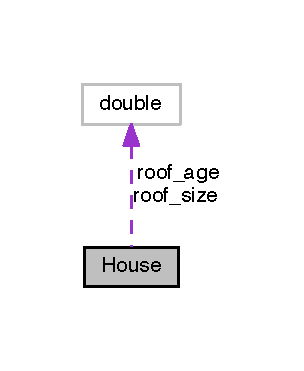
\includegraphics[width=146pt]{class_house__coll__graph}
\end{center}
\end{figure}
\subsection*{Public Attributes}
\begin{DoxyCompactItemize}
\item 
double \hyperlink{class_house_a30c17e1166d2dcb0514d6fc25f7c9e9d}{roof\+\_\+age}
\item 
double \hyperlink{class_house_a8b9b7814c17814f6df74c5bfb13d5b74}{roof\+\_\+size}
\end{DoxyCompactItemize}


\subsection{Detailed Description}
M\+A\+R\+K\+: generally have 2-\/d grid for spacial information, but it might be too much for the number of agents. Might need to compress or block representation. 10$^\wedge$5 = 10$^\wedge$3 $\ast$ 10$^\wedge$3. Might need grid with sizes, each lot has a size. 10$^\wedge$3 for rows and columns is O\+K size.

Will have patches of houses, each house -\/ 1 tile with size. Also will have empty tiles with sizes also. Will decrease total number of tiles. Will have neighborhoods with different tile sizes, house characteristics, population density as a derivative of tile size.

Belongs to Household. 

Definition at line 32 of file Geography.\+h.



\subsection{Member Data Documentation}
\hypertarget{class_house_a30c17e1166d2dcb0514d6fc25f7c9e9d}{}\index{House@{House}!roof\+\_\+age@{roof\+\_\+age}}
\index{roof\+\_\+age@{roof\+\_\+age}!House@{House}}
\subsubsection[{roof\+\_\+age}]{\setlength{\rightskip}{0pt plus 5cm}double House\+::roof\+\_\+age}\label{class_house_a30c17e1166d2dcb0514d6fc25f7c9e9d}
age of a house roof in years (not required to be whole years) 

Definition at line 35 of file Geography.\+h.

\hypertarget{class_house_a8b9b7814c17814f6df74c5bfb13d5b74}{}\index{House@{House}!roof\+\_\+size@{roof\+\_\+size}}
\index{roof\+\_\+size@{roof\+\_\+size}!House@{House}}
\subsubsection[{roof\+\_\+size}]{\setlength{\rightskip}{0pt plus 5cm}double House\+::roof\+\_\+size}\label{class_house_a8b9b7814c17814f6df74c5bfb13d5b74}
size of a roof, in m$^\wedge$2 

Definition at line 36 of file Geography.\+h.



The documentation for this class was generated from the following file\+:\begin{DoxyCompactItemize}
\item 
/\+Users/wilfeli/\+Dropbox/\+A\+B\+M/\+Solar\+Panels/\+A\+B\+M\+I\+R\+I\+S\+Lab/\+Source/\+Geography/\hyperlink{_geography_8h}{Geography.\+h}\end{DoxyCompactItemize}

\hypertarget{classsolar__core_1_1_household}{}\section{solar\+\_\+core\+:\+:Household Class Reference}
\label{classsolar__core_1_1_household}\index{solar\+\_\+core\+::\+Household@{solar\+\_\+core\+::\+Household}}


{\ttfamily \#include $<$H.\+h$>$}



Inheritance diagram for solar\+\_\+core\+:\+:Household\+:\nopagebreak
\begin{figure}[H]
\begin{center}
\leavevmode
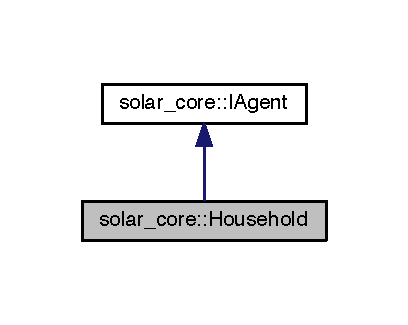
\includegraphics[width=196pt]{classsolar__core_1_1_household__inherit__graph}
\end{center}
\end{figure}


Collaboration diagram for solar\+\_\+core\+:\+:Household\+:
\nopagebreak
\begin{figure}[H]
\begin{center}
\leavevmode
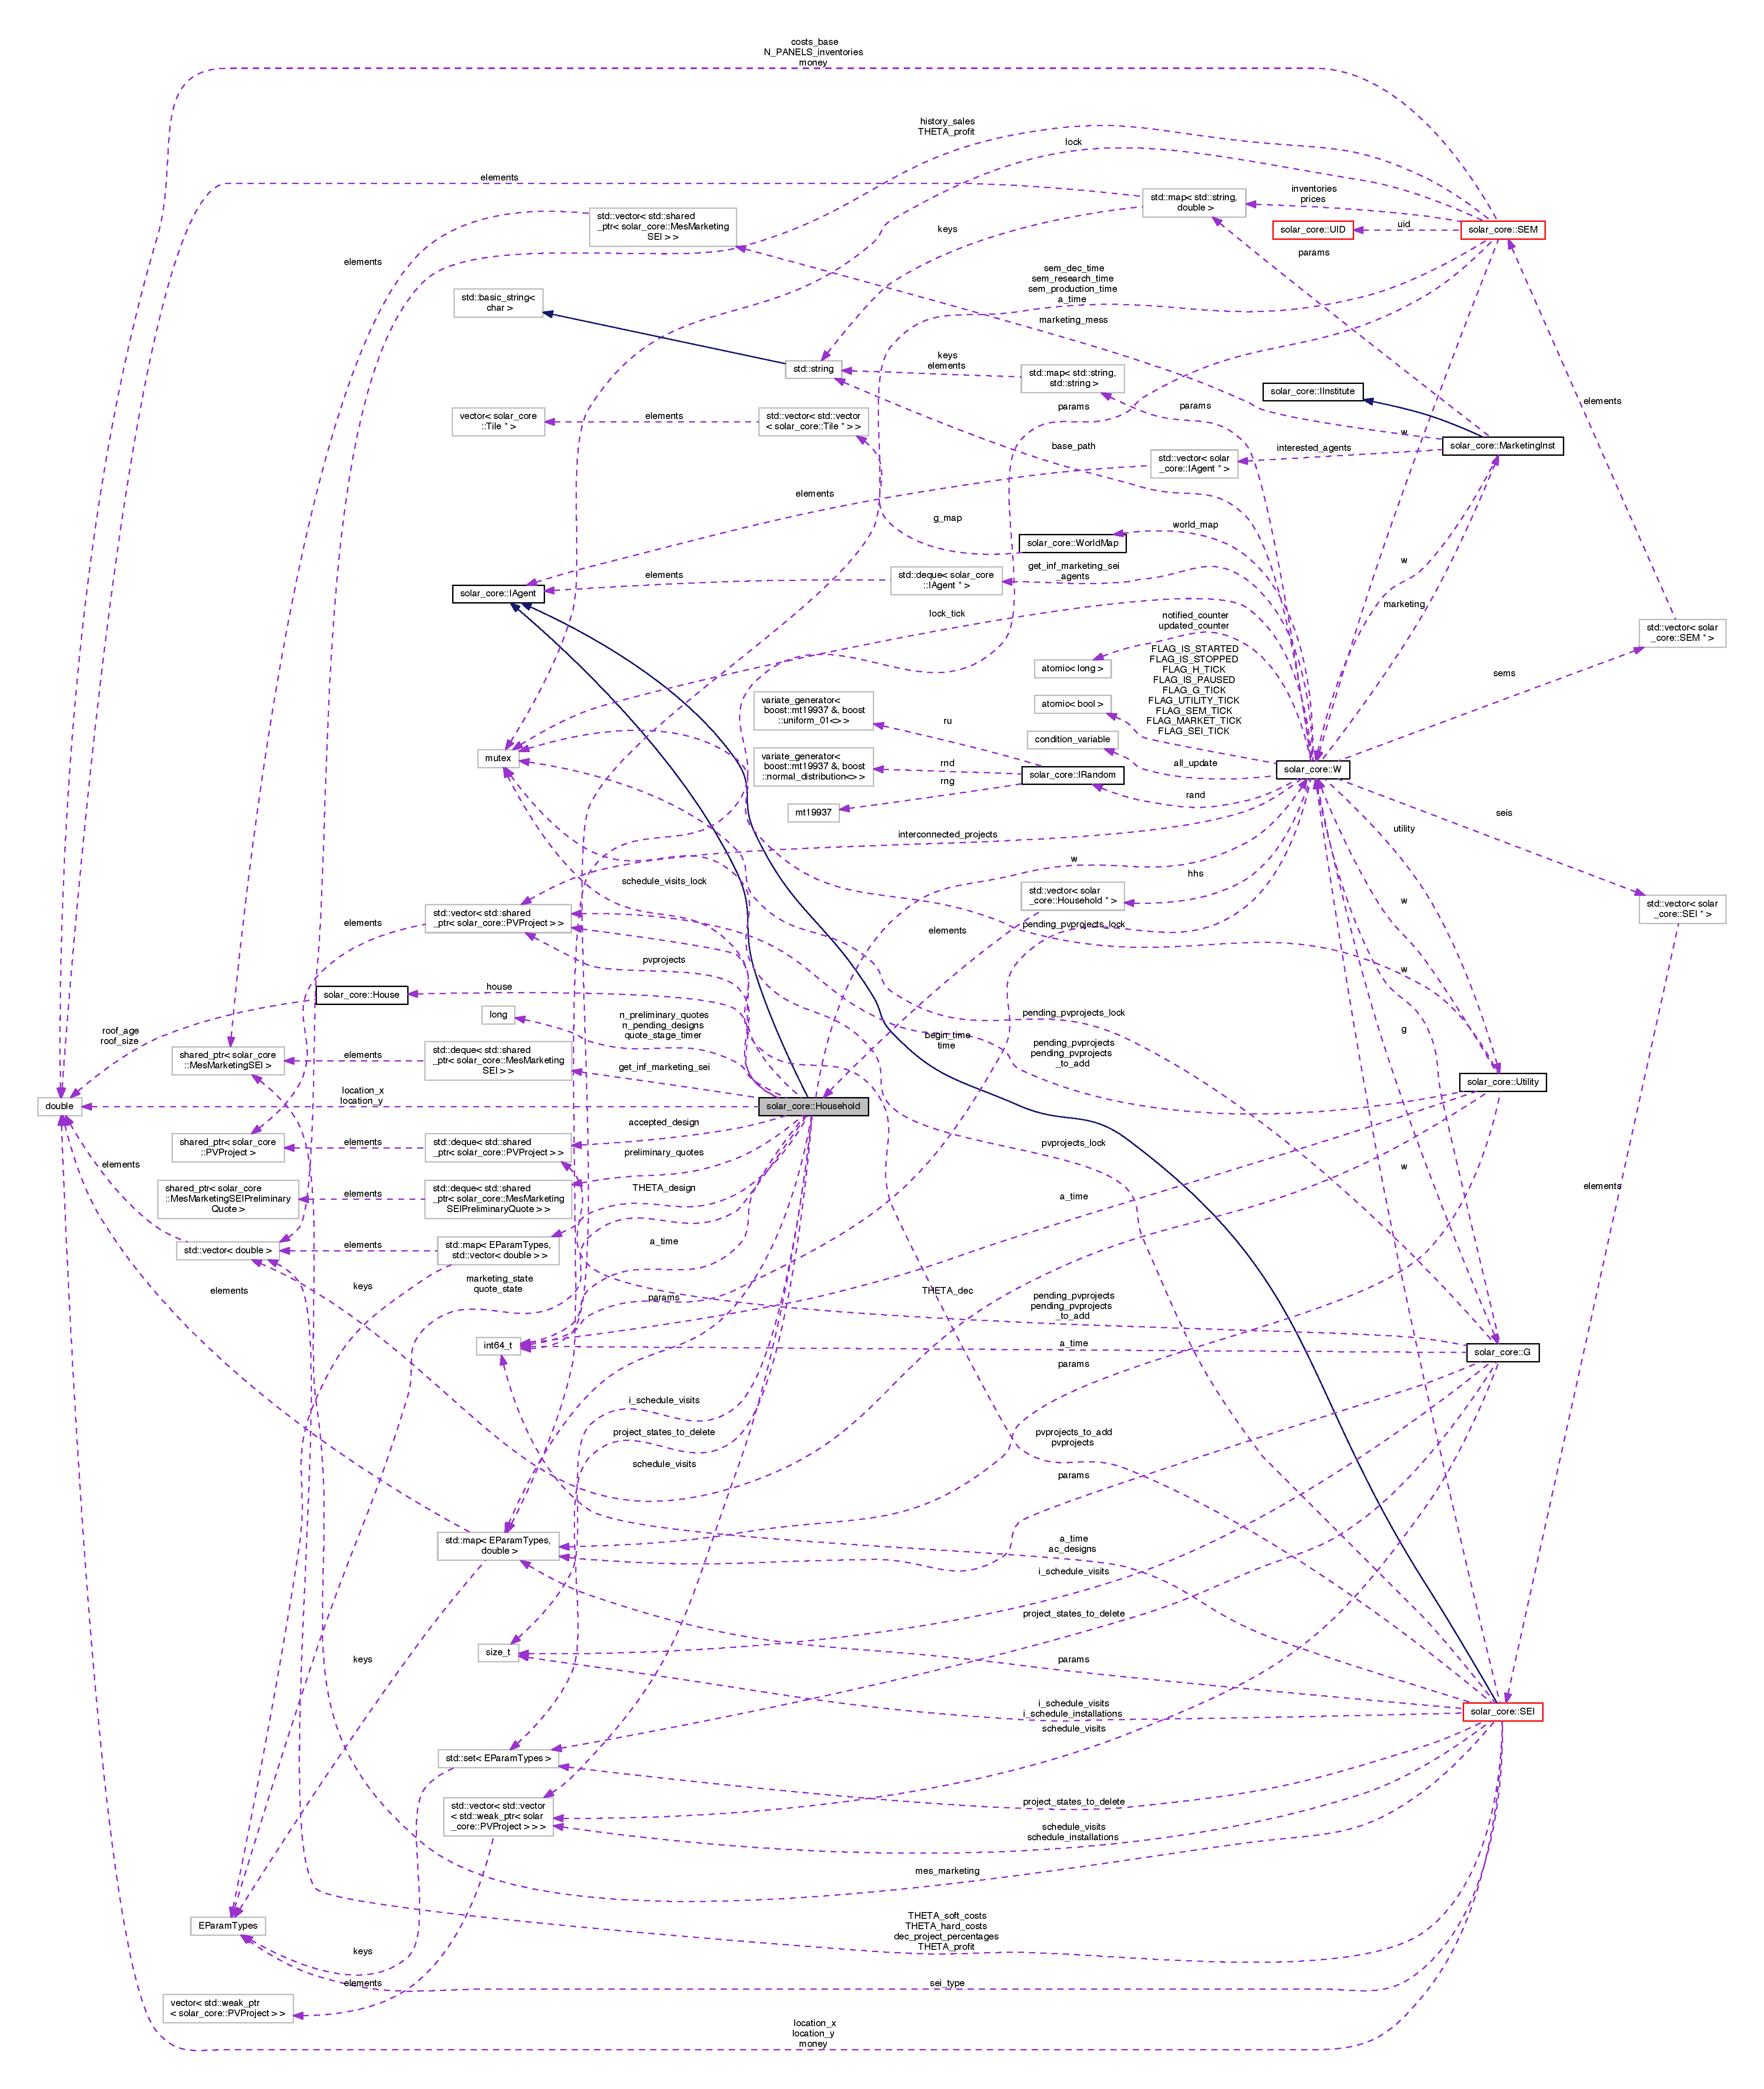
\includegraphics[width=350pt]{classsolar__core_1_1_household__coll__graph}
\end{center}
\end{figure}
\subsection*{Public Member Functions}
{\bf }\par
\begin{DoxyCompactItemize}
\item 
virtual void \hyperlink{classsolar__core_1_1_household_a165b7c64c72e5ed4ea08307e32082517}{ac\+\_\+inf\+\_\+quoting\+\_\+sei} ()
\item 
virtual void \hyperlink{classsolar__core_1_1_household_a1e7d20a60dc42b8d09a8d23a4cdb26a6}{act\+\_\+tick} ()
\end{DoxyCompactItemize}

{\bf }\par
\begin{DoxyCompactItemize}
\item 
virtual void \hyperlink{classsolar__core_1_1_household_ac9d26af7b52f0cdc357fc5dca4b86ad9}{get\+\_\+inf} (std\+::shared\+\_\+ptr$<$ \hyperlink{classsolar__core_1_1_mes_marketing_s_e_i}{Mes\+Marketing\+S\+E\+I} $>$ mes\+\_\+) override
\end{DoxyCompactItemize}

{\bf }\par
\begin{DoxyCompactItemize}
\item 
virtual std\+::shared\+\_\+ptr$<$ \hyperlink{classsolar__core_1_1_mes_state_base_h_h}{Mes\+State\+Base\+H\+H} $>$ \hyperlink{classsolar__core_1_1_household_a008a18ff8c2d15da72e19876dc896a4e}{get\+\_\+inf\+\_\+online\+\_\+quote} (\hyperlink{classsolar__core_1_1_i_agent}{I\+Agent} $\ast$agent\+\_\+to)
\item 
virtual void \hyperlink{classsolar__core_1_1_household_a31a1c8d006fb9e95a2460aa392eaa830}{receive\+\_\+preliminary\+\_\+quote} (std\+::shared\+\_\+ptr$<$ \hyperlink{classsolar__core_1_1_p_v_project}{P\+V\+Project} $>$ project\+\_\+)
\item 
virtual void \hyperlink{classsolar__core_1_1_household_a306aed410a39e8062ab5f1b4a3216b8b}{receive\+\_\+online\+\_\+quote} (std\+::shared\+\_\+ptr$<$ \hyperlink{classsolar__core_1_1_p_v_project}{P\+V\+Project} $>$ project\+\_\+)
\item 
virtual bool \hyperlink{classsolar__core_1_1_household_a8c9635bac11c9bd93e65dbb5be5b9d85}{request\+\_\+time\+\_\+slot\+\_\+visit} (\hyperlink{namespacesolar__core_a4b5949d07259da6f8a20d12a30403e90}{Time\+Unit} visit\+\_\+time, std\+::weak\+\_\+ptr$<$ \hyperlink{classsolar__core_1_1_p_v_project}{P\+V\+Project} $>$ project)
\item 
virtual bool \hyperlink{classsolar__core_1_1_household_a8d4b9c4a5cf59c93f33489eccbfba7db}{schedule\+\_\+visit} (\hyperlink{namespacesolar__core_a4b5949d07259da6f8a20d12a30403e90}{Time\+Unit} visit\+\_\+time, std\+::weak\+\_\+ptr$<$ \hyperlink{classsolar__core_1_1_p_v_project}{P\+V\+Project} $>$ project)
\item 
virtual bool \hyperlink{classsolar__core_1_1_household_aa63241ca3fcc1f2374d10b5c7f44124a}{dec\+\_\+project\+\_\+reroof} (std\+::shared\+\_\+ptr$<$ \hyperlink{classsolar__core_1_1_p_v_project}{P\+V\+Project} $>$ project)
\end{DoxyCompactItemize}

{\bf }\par
\begin{DoxyCompactItemize}
\item 
virtual void \hyperlink{classsolar__core_1_1_household_a7df346780d3d9683293af565d5831d05}{receive\+\_\+design} (std\+::shared\+\_\+ptr$<$ \hyperlink{classsolar__core_1_1_p_v_project}{P\+V\+Project} $>$ project\+\_\+)
\end{DoxyCompactItemize}

\subsection*{Public Attributes}
{\bf }\par
\begin{DoxyCompactItemize}
\item 
double \hyperlink{classsolar__core_1_1_household_a6596375631a366fdd24270f75548841f}{location\+\_\+x}
\item 
double \hyperlink{classsolar__core_1_1_household_a1ba6b7af82982096e05d99a70a2647eb}{location\+\_\+y}
\end{DoxyCompactItemize}

{\bf }\par
\begin{DoxyCompactItemize}
\item 
\hyperlink{classsolar__core_1_1_house}{House} $\ast$ \hyperlink{classsolar__core_1_1_household_a1104d8264fe733937e1fd2e9ad0f8fc1}{house}
\end{DoxyCompactItemize}

\subsection*{Protected Attributes}
{\bf }\par
\begin{DoxyCompactItemize}
\item 
std\+::map$<$ \hyperlink{namespacesolar__core_aa1147341e5ef7a40d68d1bd68e149362}{E\+Param\+Types}, double $>$ \hyperlink{classsolar__core_1_1_household_a41d61dc3bab971cb19170341b77d9df8}{params}
\end{DoxyCompactItemize}

{\bf }\par
\begin{DoxyCompactItemize}
\item 
std\+::vector$<$ std\+::shared\+\_\+ptr$<$ \hyperlink{classsolar__core_1_1_p_v_project}{P\+V\+Project} $>$ $>$ \hyperlink{classsolar__core_1_1_household_a79c0e955af98669487e0fb472811f842}{pvprojects}
\end{DoxyCompactItemize}

{\bf }\par
\begin{DoxyCompactItemize}
\item 
std\+::deque$<$ std\+::shared\+\_\+ptr$<$ \hyperlink{classsolar__core_1_1_mes_marketing_s_e_i}{Mes\+Marketing\+S\+E\+I} $>$ $>$ \hyperlink{classsolar__core_1_1_household_a3ae4cec5fca43ee5ca3287a01f5a05a2}{get\+\_\+inf\+\_\+marketing\+\_\+sei}
\item 
std\+::deque$<$ std\+::shared\+\_\+ptr$<$ \hyperlink{classsolar__core_1_1_mes_marketing_s_e_i_preliminary_quote}{Mes\+Marketing\+S\+E\+I\+Preliminary\+Quote} $>$ $>$ \hyperlink{classsolar__core_1_1_household_a297842358a2d79db160566106972bc0d}{preliminary\+\_\+quotes}
\item 
\hyperlink{namespacesolar__core_aa1147341e5ef7a40d68d1bd68e149362}{E\+Param\+Types} \hyperlink{classsolar__core_1_1_household_a3ee8b2654cad46236d11f85a4ccd9574}{marketing\+\_\+state}
\end{DoxyCompactItemize}

{\bf }\par
\begin{DoxyCompactItemize}
\item 
\hyperlink{namespacesolar__core_aa1147341e5ef7a40d68d1bd68e149362}{E\+Param\+Types} \hyperlink{classsolar__core_1_1_household_a4ae618de9a28895317824b185b57ab24}{quote\+\_\+state}
\item 
std\+::vector$<$ std\+::vector$<$ std\+::weak\+\_\+ptr$<$ \hyperlink{classsolar__core_1_1_p_v_project}{P\+V\+Project} $>$ $>$ $>$ \hyperlink{classsolar__core_1_1_household_aadd4e3e2fc66ed214bcfadf37f557b14}{schedule\+\_\+visits}
\item 
std\+::size\+\_\+t \hyperlink{classsolar__core_1_1_household_a077c668f06c009a43c535f1ad92cf92e}{i\+\_\+schedule\+\_\+visits}
\item 
std\+::mutex \hyperlink{classsolar__core_1_1_household_a15e598cfc419040a23f75fe08a8ef1d8}{schedule\+\_\+visits\+\_\+lock}
\item 
long \hyperlink{classsolar__core_1_1_household_a6b35426fd691daa6d352ec34a6ec6e4d}{quote\+\_\+stage\+\_\+timer}
\item 
long \hyperlink{classsolar__core_1_1_household_aedfc08b7837a3e2fa6ad9e62309694f3}{n\+\_\+preliminary\+\_\+quotes}
\end{DoxyCompactItemize}

{\bf }\par
\begin{DoxyCompactItemize}
\item 
std\+::deque$<$ std\+::shared\+\_\+ptr$<$ \hyperlink{classsolar__core_1_1_p_v_project}{P\+V\+Project} $>$ $>$ \hyperlink{classsolar__core_1_1_household_ad4409e81251bdd33d9dca1cd1225dc75}{accepted\+\_\+design}
\item 
long \hyperlink{classsolar__core_1_1_household_ac82a6ebca38ecaf971845f6fa5791559}{n\+\_\+pending\+\_\+designs}
\end{DoxyCompactItemize}

{\bf }\par
\begin{DoxyCompactItemize}
\item 
\hyperlink{classsolar__core_1_1_w}{W} $\ast$ \hyperlink{classsolar__core_1_1_household_a01ac4643c725f397ba7485209a906e4d}{w}
\end{DoxyCompactItemize}

\begin{DoxyCompactItemize}
\item 
\hyperlink{namespacesolar__core_a4b5949d07259da6f8a20d12a30403e90}{Time\+Unit} \hyperlink{classsolar__core_1_1_household_ad323100235079f34537ccda656e86e64}{a\+\_\+time}
\item 
virtual void \hyperlink{classsolar__core_1_1_household_a2d8c80f6db68610fb3e0f9b48e1e490b}{dec\+\_\+evaluate\+\_\+online\+\_\+quotes} ()
\item 
virtual void \hyperlink{classsolar__core_1_1_household_a6e27e36f623bd307eedcd97c550d5c5e}{dec\+\_\+evaluate\+\_\+preliminary\+\_\+quotes} ()
\item 
virtual void \hyperlink{classsolar__core_1_1_household_a733a90456d57f698b3aa974c6c6e0108}{update\+\_\+params} ()
\item 
virtual void \hyperlink{classsolar__core_1_1_household_ac73de13d0d4b4e01b2defbb85872c4b2}{ac\+\_\+update\+\_\+tick} ()
\end{DoxyCompactItemize}


\subsection{Detailed Description}
Has multiple humans, but they are not modelled as decision agents only the H\+H is the decision making agent.

\begin{DoxyRefDesc}{Solar W\+P}
\item[\hyperlink{wp__wp000001}{Solar W\+P}]Once survey is completed will have data\+: what are your choices and decisions on solar panels. The same logic as in \hyperlink{classsolar__core_1_1_s_e_i}{S\+E\+I}. Hidden parameter/factor is utility of accepting project. Might be more complex to estimate as will have a lot of categorical data.\end{DoxyRefDesc}


\begin{DoxyRefDesc}{Dev\+Stage3}
\item[\hyperlink{_dev_stage3__DevStage3000002}{Dev\+Stage3}]think about using \href{http://en.cppreference.com/w/cpp/types/result_of}{\tt http\+://en.\+cppreference.\+com/w/cpp/types/result\+\_\+of} -\/ very neat construction\end{DoxyRefDesc}


\begin{DoxyRefDesc}{Dev\+Stage2}
\item[\hyperlink{_dev_stage2__DevStage2000004}{Dev\+Stage2}]might change from actually assigning house to assigning house type (memory considerations)\end{DoxyRefDesc}


Definition at line 47 of file H.\+h.



\subsection{Member Function Documentation}
\hypertarget{classsolar__core_1_1_household_a165b7c64c72e5ed4ea08307e32082517}{}\index{solar\+\_\+core\+::\+Household@{solar\+\_\+core\+::\+Household}!ac\+\_\+inf\+\_\+quoting\+\_\+sei@{ac\+\_\+inf\+\_\+quoting\+\_\+sei}}
\index{ac\+\_\+inf\+\_\+quoting\+\_\+sei@{ac\+\_\+inf\+\_\+quoting\+\_\+sei}!solar\+\_\+core\+::\+Household@{solar\+\_\+core\+::\+Household}}
\subsubsection[{ac\+\_\+inf\+\_\+quoting\+\_\+sei}]{\setlength{\rightskip}{0pt plus 5cm}void Household\+::ac\+\_\+inf\+\_\+quoting\+\_\+sei (
\begin{DoxyParamCaption}
{}
\end{DoxyParamCaption}
)\hspace{0.3cm}{\ttfamily [virtual]}}\label{classsolar__core_1_1_household_a165b7c64c72e5ed4ea08307e32082517}
Creation and initialization section

\begin{DoxyRefDesc}{Dev\+Stage2}
\item[\hyperlink{_dev_stage2__DevStage2000005}{Dev\+Stage2}]need destructor, copy constructor, copy assignment operator, move constructor, move assignment operator\end{DoxyRefDesc}


C(const C\&) = default; // Copy constructor C(\+C\&\&) = default; // Move constructor C\& operator=(const C\&) \& = default; // Copy assignment operator C\& operator=(\+C\&\&) \& = default; // Move assignment operator virtual $\sim$\+C() \{ \} // Destructor

see \href{http://stackoverflow.com/questions/4782757/rule-of-three-becomes-rule-of-five-with-c11}{\tt http\+://stackoverflow.\+com/questions/4782757/rule-\/of-\/three-\/becomes-\/rule-\/of-\/five-\/with-\/c11}

Section with actions in the worldaction to request information from \hyperlink{classsolar__core_1_1_s_e_i}{S\+E\+I} when initiative is given from the \hyperlink{classsolar__core_1_1_w}{W} \begin{DoxyRefDesc}{Dev\+Stage2}
\item[\hyperlink{_dev_stage2__DevStage2000002}{Dev\+Stage2}]think about moving difference to the virtual call. For now it is explicit, as it is assumed that agents themselves realize that it will be online vs offline quote \end{DoxyRefDesc}


Definition at line 40 of file H.\+cpp.



Here is the call graph for this function\+:
\nopagebreak
\begin{figure}[H]
\begin{center}
\leavevmode
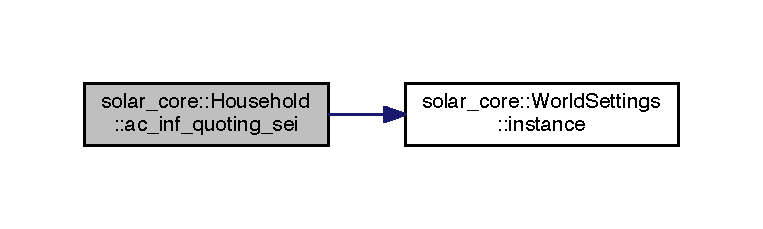
\includegraphics[width=350pt]{classsolar__core_1_1_household_a165b7c64c72e5ed4ea08307e32082517_cgraph}
\end{center}
\end{figure}




Here is the caller graph for this function\+:
\nopagebreak
\begin{figure}[H]
\begin{center}
\leavevmode
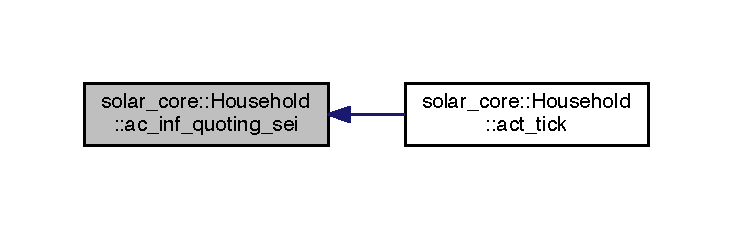
\includegraphics[width=350pt]{classsolar__core_1_1_household_a165b7c64c72e5ed4ea08307e32082517_icgraph}
\end{center}
\end{figure}


\hypertarget{classsolar__core_1_1_household_ac73de13d0d4b4e01b2defbb85872c4b2}{}\index{solar\+\_\+core\+::\+Household@{solar\+\_\+core\+::\+Household}!ac\+\_\+update\+\_\+tick@{ac\+\_\+update\+\_\+tick}}
\index{ac\+\_\+update\+\_\+tick@{ac\+\_\+update\+\_\+tick}!solar\+\_\+core\+::\+Household@{solar\+\_\+core\+::\+Household}}
\subsubsection[{ac\+\_\+update\+\_\+tick}]{\setlength{\rightskip}{0pt plus 5cm}void Household\+::ac\+\_\+update\+\_\+tick (
\begin{DoxyParamCaption}
{}
\end{DoxyParamCaption}
)\hspace{0.3cm}{\ttfamily [protected]}, {\ttfamily [virtual]}}\label{classsolar__core_1_1_household_ac73de13d0d4b4e01b2defbb85872c4b2}
update internals for the tick 

Definition at line 265 of file H.\+cpp.



Here is the call graph for this function\+:
\nopagebreak
\begin{figure}[H]
\begin{center}
\leavevmode
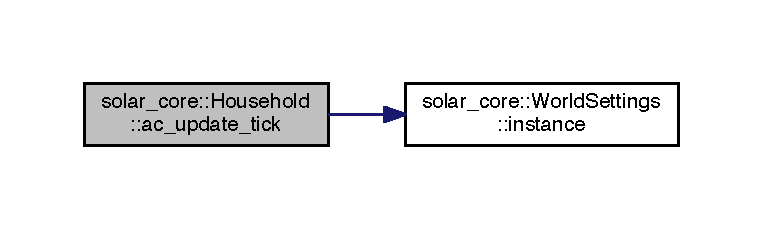
\includegraphics[width=350pt]{classsolar__core_1_1_household_ac73de13d0d4b4e01b2defbb85872c4b2_cgraph}
\end{center}
\end{figure}




Here is the caller graph for this function\+:
\nopagebreak
\begin{figure}[H]
\begin{center}
\leavevmode
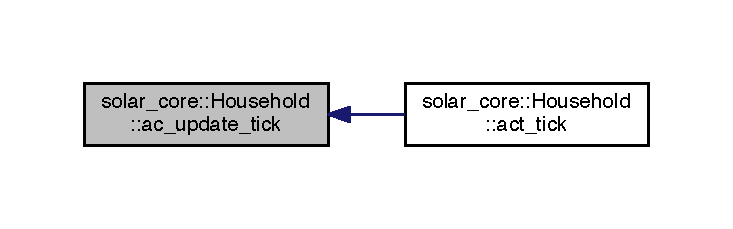
\includegraphics[width=350pt]{classsolar__core_1_1_household_ac73de13d0d4b4e01b2defbb85872c4b2_icgraph}
\end{center}
\end{figure}


\hypertarget{classsolar__core_1_1_household_a1e7d20a60dc42b8d09a8d23a4cdb26a6}{}\index{solar\+\_\+core\+::\+Household@{solar\+\_\+core\+::\+Household}!act\+\_\+tick@{act\+\_\+tick}}
\index{act\+\_\+tick@{act\+\_\+tick}!solar\+\_\+core\+::\+Household@{solar\+\_\+core\+::\+Household}}
\subsubsection[{act\+\_\+tick}]{\setlength{\rightskip}{0pt plus 5cm}void Household\+::act\+\_\+tick (
\begin{DoxyParamCaption}
{}
\end{DoxyParamCaption}
)\hspace{0.3cm}{\ttfamily [virtual]}}\label{classsolar__core_1_1_household_a1e7d20a60dc42b8d09a8d23a4cdb26a6}
generic actions on a tick, specialize for each type of agents generally actions in a tick depend on the state of an agent, either it is choosing installer or waiting for the project to finish. Might have a call back to w that will indicate that this agent has changed state. In this case w will have multiple lists of agents in different states and would call appropriate function. Or might do it internally where new state will dictate behavior in the tick. Generally have both -\/ agent is broadcasting changed state and behaves differently depending on the state. 

Implements \hyperlink{classsolar__core_1_1_i_agent_a6813e8e4f94ab2dc917a29c4d6609149}{solar\+\_\+core\+::\+I\+Agent}.



Definition at line 291 of file H.\+cpp.



Here is the call graph for this function\+:
\nopagebreak
\begin{figure}[H]
\begin{center}
\leavevmode
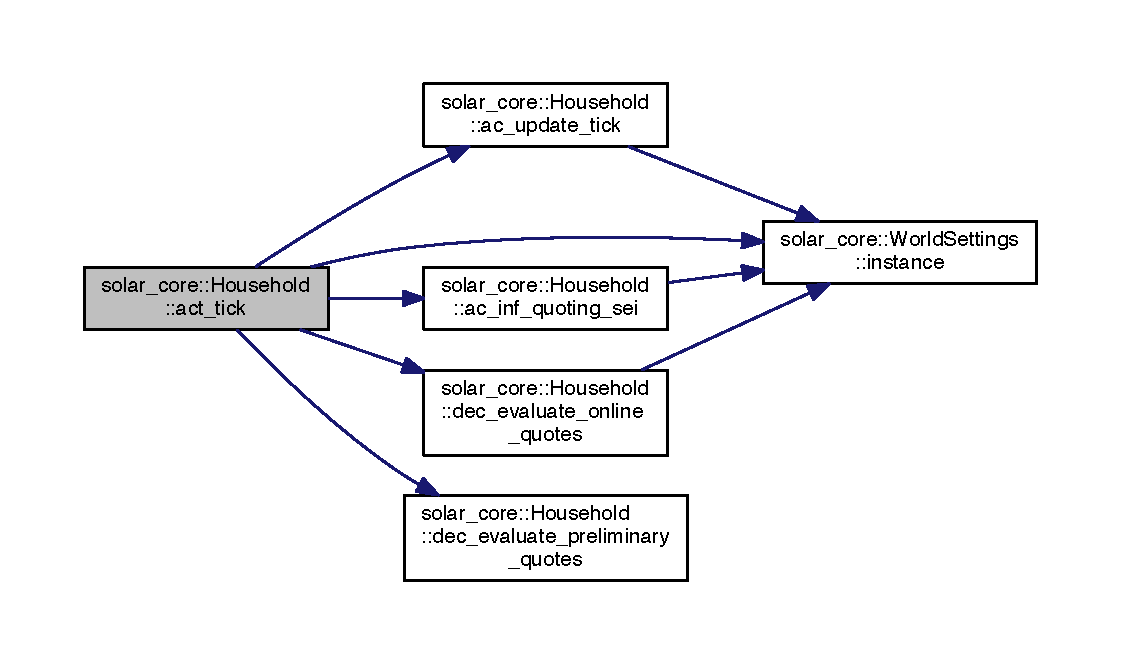
\includegraphics[width=350pt]{classsolar__core_1_1_household_a1e7d20a60dc42b8d09a8d23a4cdb26a6_cgraph}
\end{center}
\end{figure}


\hypertarget{classsolar__core_1_1_household_a2d8c80f6db68610fb3e0f9b48e1e490b}{}\index{solar\+\_\+core\+::\+Household@{solar\+\_\+core\+::\+Household}!dec\+\_\+evaluate\+\_\+online\+\_\+quotes@{dec\+\_\+evaluate\+\_\+online\+\_\+quotes}}
\index{dec\+\_\+evaluate\+\_\+online\+\_\+quotes@{dec\+\_\+evaluate\+\_\+online\+\_\+quotes}!solar\+\_\+core\+::\+Household@{solar\+\_\+core\+::\+Household}}
\subsubsection[{dec\+\_\+evaluate\+\_\+online\+\_\+quotes}]{\setlength{\rightskip}{0pt plus 5cm}void Household\+::dec\+\_\+evaluate\+\_\+online\+\_\+quotes (
\begin{DoxyParamCaption}
{}
\end{DoxyParamCaption}
)\hspace{0.3cm}{\ttfamily [protected]}, {\ttfamily [virtual]}}\label{classsolar__core_1_1_household_a2d8c80f6db68610fb3e0f9b48e1e490b}
Section with agent\textquotesingle{}s internalseveluate online quotes -\/ which to be persued further 

Definition at line 100 of file H.\+cpp.



Here is the call graph for this function\+:
\nopagebreak
\begin{figure}[H]
\begin{center}
\leavevmode
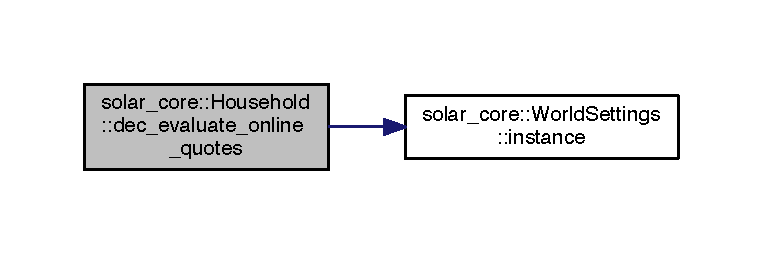
\includegraphics[width=350pt]{classsolar__core_1_1_household_a2d8c80f6db68610fb3e0f9b48e1e490b_cgraph}
\end{center}
\end{figure}




Here is the caller graph for this function\+:
\nopagebreak
\begin{figure}[H]
\begin{center}
\leavevmode
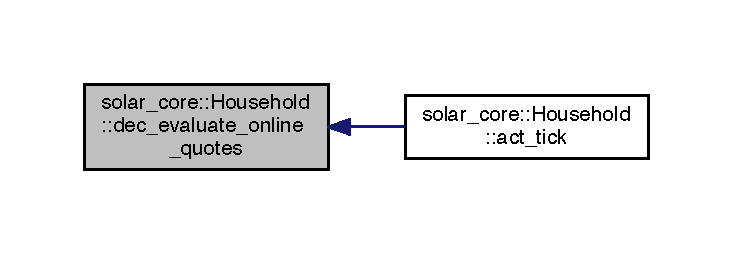
\includegraphics[width=350pt]{classsolar__core_1_1_household_a2d8c80f6db68610fb3e0f9b48e1e490b_icgraph}
\end{center}
\end{figure}


\hypertarget{classsolar__core_1_1_household_a6e27e36f623bd307eedcd97c550d5c5e}{}\index{solar\+\_\+core\+::\+Household@{solar\+\_\+core\+::\+Household}!dec\+\_\+evaluate\+\_\+preliminary\+\_\+quotes@{dec\+\_\+evaluate\+\_\+preliminary\+\_\+quotes}}
\index{dec\+\_\+evaluate\+\_\+preliminary\+\_\+quotes@{dec\+\_\+evaluate\+\_\+preliminary\+\_\+quotes}!solar\+\_\+core\+::\+Household@{solar\+\_\+core\+::\+Household}}
\subsubsection[{dec\+\_\+evaluate\+\_\+preliminary\+\_\+quotes}]{\setlength{\rightskip}{0pt plus 5cm}void Household\+::dec\+\_\+evaluate\+\_\+preliminary\+\_\+quotes (
\begin{DoxyParamCaption}
{}
\end{DoxyParamCaption}
)\hspace{0.3cm}{\ttfamily [protected]}, {\ttfamily [virtual]}}\label{classsolar__core_1_1_household_a6e27e36f623bd307eedcd97c550d5c5e}
eveluate preliminary quotes -\/ which to be persued further  G\+U\+I\+D research. Boost G\+U\+I\+D is almost unique, uses machine and time, so could be repeated if used across machines or time is changed 

Definition at line 131 of file H.\+cpp.



Here is the caller graph for this function\+:
\nopagebreak
\begin{figure}[H]
\begin{center}
\leavevmode
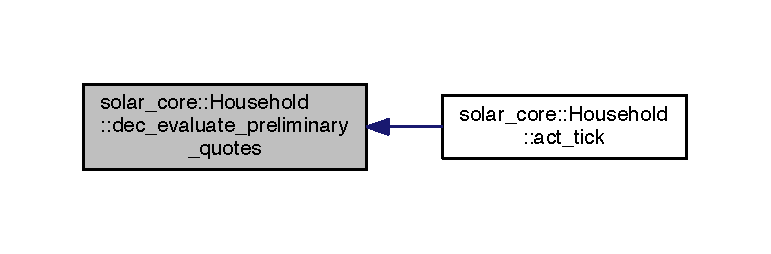
\includegraphics[width=350pt]{classsolar__core_1_1_household_a6e27e36f623bd307eedcd97c550d5c5e_icgraph}
\end{center}
\end{figure}


\hypertarget{classsolar__core_1_1_household_aa63241ca3fcc1f2374d10b5c7f44124a}{}\index{solar\+\_\+core\+::\+Household@{solar\+\_\+core\+::\+Household}!dec\+\_\+project\+\_\+reroof@{dec\+\_\+project\+\_\+reroof}}
\index{dec\+\_\+project\+\_\+reroof@{dec\+\_\+project\+\_\+reroof}!solar\+\_\+core\+::\+Household@{solar\+\_\+core\+::\+Household}}
\subsubsection[{dec\+\_\+project\+\_\+reroof}]{\setlength{\rightskip}{0pt plus 5cm}bool Household\+::dec\+\_\+project\+\_\+reroof (
\begin{DoxyParamCaption}
\item[{std\+::shared\+\_\+ptr$<$ {\bf P\+V\+Project} $>$}]{project}
\end{DoxyParamCaption}
)\hspace{0.3cm}{\ttfamily [virtual]}}\label{classsolar__core_1_1_household_aa63241ca3fcc1f2374d10b5c7f44124a}
\begin{DoxyRefDesc}{Solar W\+P}
\item[\hyperlink{wp__wp000002}{Solar W\+P}]need to ask H\+H how they decide to reroof \end{DoxyRefDesc}


Definition at line 256 of file H.\+cpp.

\hypertarget{classsolar__core_1_1_household_ac9d26af7b52f0cdc357fc5dca4b86ad9}{}\index{solar\+\_\+core\+::\+Household@{solar\+\_\+core\+::\+Household}!get\+\_\+inf@{get\+\_\+inf}}
\index{get\+\_\+inf@{get\+\_\+inf}!solar\+\_\+core\+::\+Household@{solar\+\_\+core\+::\+Household}}
\subsubsection[{get\+\_\+inf}]{\setlength{\rightskip}{0pt plus 5cm}void Household\+::get\+\_\+inf (
\begin{DoxyParamCaption}
\item[{std\+::shared\+\_\+ptr$<$ {\bf Mes\+Marketing\+S\+E\+I} $>$}]{mes\+\_\+}
\end{DoxyParamCaption}
)\hspace{0.3cm}{\ttfamily [override]}, {\ttfamily [virtual]}}\label{classsolar__core_1_1_household_ac9d26af7b52f0cdc357fc5dca4b86ad9}
Section relevant to marketing informationreceives marketing information No mutex guards as only other operation is poping from the front, which does not invalidate anything

\begin{DoxyRefDesc}{Dev\+Stage2}
\item[\hyperlink{_dev_stage2__DevStage2000001}{Dev\+Stage2}]might be addd saving of the time of the marketing message, in this case it will be saved in the form of transformed marketing messages because original message will time stamped at the moment of creation (almost at the beginning of the simulation) \end{DoxyRefDesc}


\begin{DoxyRefDesc}{Dev\+Stage3}
\item[\hyperlink{_dev_stage3__DevStage3000001}{Dev\+Stage3}]check if this agent is interested in the marketing message \end{DoxyRefDesc}


Implements \hyperlink{classsolar__core_1_1_i_agent_aa9ebc762ed032f7084063199747decb6}{solar\+\_\+core\+::\+I\+Agent}.



Definition at line 19 of file H.\+cpp.

\hypertarget{classsolar__core_1_1_household_a008a18ff8c2d15da72e19876dc896a4e}{}\index{solar\+\_\+core\+::\+Household@{solar\+\_\+core\+::\+Household}!get\+\_\+inf\+\_\+online\+\_\+quote@{get\+\_\+inf\+\_\+online\+\_\+quote}}
\index{get\+\_\+inf\+\_\+online\+\_\+quote@{get\+\_\+inf\+\_\+online\+\_\+quote}!solar\+\_\+core\+::\+Household@{solar\+\_\+core\+::\+Household}}
\subsubsection[{get\+\_\+inf\+\_\+online\+\_\+quote}]{\setlength{\rightskip}{0pt plus 5cm}std\+::shared\+\_\+ptr$<$ {\bf Mes\+State\+Base\+H\+H} $>$ Household\+::get\+\_\+inf\+\_\+online\+\_\+quote (
\begin{DoxyParamCaption}
\item[{{\bf I\+Agent} $\ast$}]{agent\+\_\+to}
\end{DoxyParamCaption}
)\hspace{0.3cm}{\ttfamily [virtual]}}\label{classsolar__core_1_1_household_a008a18ff8c2d15da72e19876dc896a4e}
Section relevant to quoting stagefirst request for information from \hyperlink{classsolar__core_1_1_s_e_i}{S\+E\+I}, provides basic information such as credit score and etc. Some parameters need to be taken from \hyperlink{classsolar__core_1_1_house}{House} directly, they are pushed to the general container when changed 

Definition at line 215 of file H.\+cpp.



Here is the call graph for this function\+:\nopagebreak
\begin{figure}[H]
\begin{center}
\leavevmode
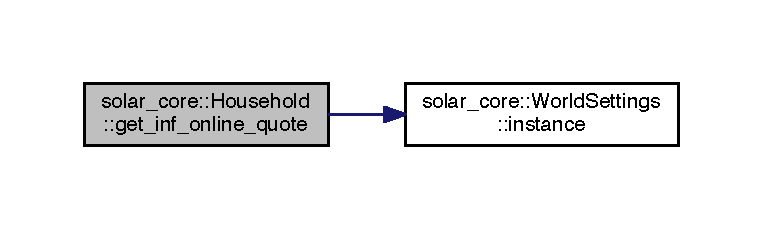
\includegraphics[width=350pt]{classsolar__core_1_1_household_a008a18ff8c2d15da72e19876dc896a4e_cgraph}
\end{center}
\end{figure}


\hypertarget{classsolar__core_1_1_household_a7df346780d3d9683293af565d5831d05}{}\index{solar\+\_\+core\+::\+Household@{solar\+\_\+core\+::\+Household}!receive\+\_\+design@{receive\+\_\+design}}
\index{receive\+\_\+design@{receive\+\_\+design}!solar\+\_\+core\+::\+Household@{solar\+\_\+core\+::\+Household}}
\subsubsection[{receive\+\_\+design}]{\setlength{\rightskip}{0pt plus 5cm}void Household\+::receive\+\_\+design (
\begin{DoxyParamCaption}
\item[{std\+::shared\+\_\+ptr$<$ {\bf P\+V\+Project} $>$}]{project\+\_\+}
\end{DoxyParamCaption}
)\hspace{0.3cm}{\ttfamily [virtual]}}\label{classsolar__core_1_1_household_a7df346780d3d9683293af565d5831d05}
Section relevant to design phaseis informed that design is received 

Definition at line 195 of file H.\+cpp.

\hypertarget{classsolar__core_1_1_household_a306aed410a39e8062ab5f1b4a3216b8b}{}\index{solar\+\_\+core\+::\+Household@{solar\+\_\+core\+::\+Household}!receive\+\_\+online\+\_\+quote@{receive\+\_\+online\+\_\+quote}}
\index{receive\+\_\+online\+\_\+quote@{receive\+\_\+online\+\_\+quote}!solar\+\_\+core\+::\+Household@{solar\+\_\+core\+::\+Household}}
\subsubsection[{receive\+\_\+online\+\_\+quote}]{\setlength{\rightskip}{0pt plus 5cm}void Household\+::receive\+\_\+online\+\_\+quote (
\begin{DoxyParamCaption}
\item[{std\+::shared\+\_\+ptr$<$ {\bf P\+V\+Project} $>$}]{project\+\_\+}
\end{DoxyParamCaption}
)\hspace{0.3cm}{\ttfamily [virtual]}}\label{classsolar__core_1_1_household_a306aed410a39e8062ab5f1b4a3216b8b}
empty for now as information is added directly to the project itself 

Definition at line 208 of file H.\+cpp.

\hypertarget{classsolar__core_1_1_household_a31a1c8d006fb9e95a2460aa392eaa830}{}\index{solar\+\_\+core\+::\+Household@{solar\+\_\+core\+::\+Household}!receive\+\_\+preliminary\+\_\+quote@{receive\+\_\+preliminary\+\_\+quote}}
\index{receive\+\_\+preliminary\+\_\+quote@{receive\+\_\+preliminary\+\_\+quote}!solar\+\_\+core\+::\+Household@{solar\+\_\+core\+::\+Household}}
\subsubsection[{receive\+\_\+preliminary\+\_\+quote}]{\setlength{\rightskip}{0pt plus 5cm}void Household\+::receive\+\_\+preliminary\+\_\+quote (
\begin{DoxyParamCaption}
\item[{std\+::shared\+\_\+ptr$<$ {\bf P\+V\+Project} $>$}]{project\+\_\+}
\end{DoxyParamCaption}
)\hspace{0.3cm}{\ttfamily [virtual]}}\label{classsolar__core_1_1_household_a31a1c8d006fb9e95a2460aa392eaa830}
empty for now as information is added directly to the project itself 

Definition at line 202 of file H.\+cpp.

\hypertarget{classsolar__core_1_1_household_a8c9635bac11c9bd93e65dbb5be5b9d85}{}\index{solar\+\_\+core\+::\+Household@{solar\+\_\+core\+::\+Household}!request\+\_\+time\+\_\+slot\+\_\+visit@{request\+\_\+time\+\_\+slot\+\_\+visit}}
\index{request\+\_\+time\+\_\+slot\+\_\+visit@{request\+\_\+time\+\_\+slot\+\_\+visit}!solar\+\_\+core\+::\+Household@{solar\+\_\+core\+::\+Household}}
\subsubsection[{request\+\_\+time\+\_\+slot\+\_\+visit}]{\setlength{\rightskip}{0pt plus 5cm}bool Household\+::request\+\_\+time\+\_\+slot\+\_\+visit (
\begin{DoxyParamCaption}
\item[{{\bf Time\+Unit}}]{visit\+\_\+time, }
\item[{std\+::weak\+\_\+ptr$<$ {\bf P\+V\+Project} $>$}]{project}
\end{DoxyParamCaption}
)\hspace{0.3cm}{\ttfamily [virtual]}}\label{classsolar__core_1_1_household_a8c9635bac11c9bd93e65dbb5be5b9d85}
check that could have a visit at this time 

Definition at line 231 of file H.\+cpp.

\hypertarget{classsolar__core_1_1_household_a8d4b9c4a5cf59c93f33489eccbfba7db}{}\index{solar\+\_\+core\+::\+Household@{solar\+\_\+core\+::\+Household}!schedule\+\_\+visit@{schedule\+\_\+visit}}
\index{schedule\+\_\+visit@{schedule\+\_\+visit}!solar\+\_\+core\+::\+Household@{solar\+\_\+core\+::\+Household}}
\subsubsection[{schedule\+\_\+visit}]{\setlength{\rightskip}{0pt plus 5cm}bool Household\+::schedule\+\_\+visit (
\begin{DoxyParamCaption}
\item[{{\bf Time\+Unit}}]{visit\+\_\+time, }
\item[{std\+::weak\+\_\+ptr$<$ {\bf P\+V\+Project} $>$}]{project}
\end{DoxyParamCaption}
)\hspace{0.3cm}{\ttfamily [virtual]}}\label{classsolar__core_1_1_household_a8d4b9c4a5cf59c93f33489eccbfba7db}
schedules visit at this time, returns false if no slots are open 

Definition at line 238 of file H.\+cpp.

\hypertarget{classsolar__core_1_1_household_a733a90456d57f698b3aa974c6c6e0108}{}\index{solar\+\_\+core\+::\+Household@{solar\+\_\+core\+::\+Household}!update\+\_\+params@{update\+\_\+params}}
\index{update\+\_\+params@{update\+\_\+params}!solar\+\_\+core\+::\+Household@{solar\+\_\+core\+::\+Household}}
\subsubsection[{update\+\_\+params}]{\setlength{\rightskip}{0pt plus 5cm}void Household\+::update\+\_\+params (
\begin{DoxyParamCaption}
{}
\end{DoxyParamCaption}
)\hspace{0.3cm}{\ttfamily [protected]}, {\ttfamily [virtual]}}\label{classsolar__core_1_1_household_a733a90456d57f698b3aa974c6c6e0108}
is called when some part of parameters is updated that is not saved in the main map with parameters. Is used to keep all parameters synchronized. 

Definition at line 341 of file H.\+cpp.



\subsection{Member Data Documentation}
\hypertarget{classsolar__core_1_1_household_ad323100235079f34537ccda656e86e64}{}\index{solar\+\_\+core\+::\+Household@{solar\+\_\+core\+::\+Household}!a\+\_\+time@{a\+\_\+time}}
\index{a\+\_\+time@{a\+\_\+time}!solar\+\_\+core\+::\+Household@{solar\+\_\+core\+::\+Household}}
\subsubsection[{a\+\_\+time}]{\setlength{\rightskip}{0pt plus 5cm}{\bf Time\+Unit} solar\+\_\+core\+::\+Household\+::a\+\_\+time\hspace{0.3cm}{\ttfamily [protected]}}\label{classsolar__core_1_1_household_ad323100235079f34537ccda656e86e64}
internal agent\textquotesingle{}s timer 

Definition at line 279 of file H.\+h.

\hypertarget{classsolar__core_1_1_household_ad4409e81251bdd33d9dca1cd1225dc75}{}\index{solar\+\_\+core\+::\+Household@{solar\+\_\+core\+::\+Household}!accepted\+\_\+design@{accepted\+\_\+design}}
\index{accepted\+\_\+design@{accepted\+\_\+design}!solar\+\_\+core\+::\+Household@{solar\+\_\+core\+::\+Household}}
\subsubsection[{accepted\+\_\+design}]{\setlength{\rightskip}{0pt plus 5cm}std\+::deque$<$std\+::shared\+\_\+ptr$<${\bf P\+V\+Project}$>$ $>$ solar\+\_\+core\+::\+Household\+::accepted\+\_\+design\hspace{0.3cm}{\ttfamily [protected]}}\label{classsolar__core_1_1_household_ad4409e81251bdd33d9dca1cd1225dc75}
Section relevant to design stage 

Definition at line 257 of file H.\+h.

\hypertarget{classsolar__core_1_1_household_a3ae4cec5fca43ee5ca3287a01f5a05a2}{}\index{solar\+\_\+core\+::\+Household@{solar\+\_\+core\+::\+Household}!get\+\_\+inf\+\_\+marketing\+\_\+sei@{get\+\_\+inf\+\_\+marketing\+\_\+sei}}
\index{get\+\_\+inf\+\_\+marketing\+\_\+sei@{get\+\_\+inf\+\_\+marketing\+\_\+sei}!solar\+\_\+core\+::\+Household@{solar\+\_\+core\+::\+Household}}
\subsubsection[{get\+\_\+inf\+\_\+marketing\+\_\+sei}]{\setlength{\rightskip}{0pt plus 5cm}std\+::deque$<$std\+::shared\+\_\+ptr$<${\bf Mes\+Marketing\+S\+E\+I}$>$ $>$ solar\+\_\+core\+::\+Household\+::get\+\_\+inf\+\_\+marketing\+\_\+sei\hspace{0.3cm}{\ttfamily [protected]}}\label{classsolar__core_1_1_household_a3ae4cec5fca43ee5ca3287a01f5a05a2}
Section relevant to marketing informationstores list of marketing infiormation from \hyperlink{classsolar__core_1_1_s_e_i}{S\+E\+I} agents that this agent is interested in geting quotes from 

Definition at line 222 of file H.\+h.

\hypertarget{classsolar__core_1_1_household_a1104d8264fe733937e1fd2e9ad0f8fc1}{}\index{solar\+\_\+core\+::\+Household@{solar\+\_\+core\+::\+Household}!house@{house}}
\index{house@{house}!solar\+\_\+core\+::\+Household@{solar\+\_\+core\+::\+Household}}
\subsubsection[{house}]{\setlength{\rightskip}{0pt plus 5cm}{\bf House}$\ast$ solar\+\_\+core\+::\+Household\+::house}\label{classsolar__core_1_1_household_a1104d8264fe733937e1fd2e9ad0f8fc1}
Location of an agent, y coordinate.\begin{DoxyRefDesc}{Dev\+Stage2}
\item[\hyperlink{_dev_stage2__DevStage2000007}{Dev\+Stage2}]think about decreasing size for this field, use uint64\+\_\+t or smaller for it \end{DoxyRefDesc}


Section with parameters for solar projects, mainly \hyperlink{classsolar__core_1_1_house}{House} for now 

Definition at line 167 of file H.\+h.

\hypertarget{classsolar__core_1_1_household_a077c668f06c009a43c535f1ad92cf92e}{}\index{solar\+\_\+core\+::\+Household@{solar\+\_\+core\+::\+Household}!i\+\_\+schedule\+\_\+visits@{i\+\_\+schedule\+\_\+visits}}
\index{i\+\_\+schedule\+\_\+visits@{i\+\_\+schedule\+\_\+visits}!solar\+\_\+core\+::\+Household@{solar\+\_\+core\+::\+Household}}
\subsubsection[{i\+\_\+schedule\+\_\+visits}]{\setlength{\rightskip}{0pt plus 5cm}std\+::size\+\_\+t solar\+\_\+core\+::\+Household\+::i\+\_\+schedule\+\_\+visits\hspace{0.3cm}{\ttfamily [protected]}}\label{classsolar__core_1_1_household_a077c668f06c009a43c535f1ad92cf92e}


Definition at line 242 of file H.\+h.

\hypertarget{classsolar__core_1_1_household_a6596375631a366fdd24270f75548841f}{}\index{solar\+\_\+core\+::\+Household@{solar\+\_\+core\+::\+Household}!location\+\_\+x@{location\+\_\+x}}
\index{location\+\_\+x@{location\+\_\+x}!solar\+\_\+core\+::\+Household@{solar\+\_\+core\+::\+Household}}
\subsubsection[{location\+\_\+x}]{\setlength{\rightskip}{0pt plus 5cm}double solar\+\_\+core\+::\+Household\+::location\+\_\+x}\label{classsolar__core_1_1_household_a6596375631a366fdd24270f75548841f}
Section with geographical parameters 

Definition at line 150 of file H.\+h.

\hypertarget{classsolar__core_1_1_household_a1ba6b7af82982096e05d99a70a2647eb}{}\index{solar\+\_\+core\+::\+Household@{solar\+\_\+core\+::\+Household}!location\+\_\+y@{location\+\_\+y}}
\index{location\+\_\+y@{location\+\_\+y}!solar\+\_\+core\+::\+Household@{solar\+\_\+core\+::\+Household}}
\subsubsection[{location\+\_\+y}]{\setlength{\rightskip}{0pt plus 5cm}double solar\+\_\+core\+::\+Household\+::location\+\_\+y}\label{classsolar__core_1_1_household_a1ba6b7af82982096e05d99a70a2647eb}
Location of an agent, x coordinate.\begin{DoxyRefDesc}{Dev\+Stage2}
\item[\hyperlink{_dev_stage2__DevStage2000006}{Dev\+Stage2}]think about decreasing size for this field, use uint64\+\_\+t or smaller for it \end{DoxyRefDesc}


Definition at line 151 of file H.\+h.

\hypertarget{classsolar__core_1_1_household_a3ee8b2654cad46236d11f85a4ccd9574}{}\index{solar\+\_\+core\+::\+Household@{solar\+\_\+core\+::\+Household}!marketing\+\_\+state@{marketing\+\_\+state}}
\index{marketing\+\_\+state@{marketing\+\_\+state}!solar\+\_\+core\+::\+Household@{solar\+\_\+core\+::\+Household}}
\subsubsection[{marketing\+\_\+state}]{\setlength{\rightskip}{0pt plus 5cm}{\bf E\+Param\+Types} solar\+\_\+core\+::\+Household\+::marketing\+\_\+state\hspace{0.3cm}{\ttfamily [protected]}}\label{classsolar__core_1_1_household_a3ee8b2654cad46236d11f85a4ccd9574}
could be interested, very interested or not 

Definition at line 226 of file H.\+h.

\hypertarget{classsolar__core_1_1_household_ac82a6ebca38ecaf971845f6fa5791559}{}\index{solar\+\_\+core\+::\+Household@{solar\+\_\+core\+::\+Household}!n\+\_\+pending\+\_\+designs@{n\+\_\+pending\+\_\+designs}}
\index{n\+\_\+pending\+\_\+designs@{n\+\_\+pending\+\_\+designs}!solar\+\_\+core\+::\+Household@{solar\+\_\+core\+::\+Household}}
\subsubsection[{n\+\_\+pending\+\_\+designs}]{\setlength{\rightskip}{0pt plus 5cm}long solar\+\_\+core\+::\+Household\+::n\+\_\+pending\+\_\+designs\hspace{0.3cm}{\ttfamily [protected]}}\label{classsolar__core_1_1_household_ac82a6ebca38ecaf971845f6fa5791559}


Definition at line 258 of file H.\+h.

\hypertarget{classsolar__core_1_1_household_aedfc08b7837a3e2fa6ad9e62309694f3}{}\index{solar\+\_\+core\+::\+Household@{solar\+\_\+core\+::\+Household}!n\+\_\+preliminary\+\_\+quotes@{n\+\_\+preliminary\+\_\+quotes}}
\index{n\+\_\+preliminary\+\_\+quotes@{n\+\_\+preliminary\+\_\+quotes}!solar\+\_\+core\+::\+Household@{solar\+\_\+core\+::\+Household}}
\subsubsection[{n\+\_\+preliminary\+\_\+quotes}]{\setlength{\rightskip}{0pt plus 5cm}long solar\+\_\+core\+::\+Household\+::n\+\_\+preliminary\+\_\+quotes\hspace{0.3cm}{\ttfamily [protected]}}\label{classsolar__core_1_1_household_aedfc08b7837a3e2fa6ad9e62309694f3}
number of preliminary quotes 

Definition at line 246 of file H.\+h.

\hypertarget{classsolar__core_1_1_household_a41d61dc3bab971cb19170341b77d9df8}{}\index{solar\+\_\+core\+::\+Household@{solar\+\_\+core\+::\+Household}!params@{params}}
\index{params@{params}!solar\+\_\+core\+::\+Household@{solar\+\_\+core\+::\+Household}}
\subsubsection[{params}]{\setlength{\rightskip}{0pt plus 5cm}std\+::map$<${\bf E\+Param\+Types}, double$>$ solar\+\_\+core\+::\+Household\+::params\hspace{0.3cm}{\ttfamily [protected]}}\label{classsolar__core_1_1_household_a41d61dc3bab971cb19170341b77d9df8}
Simplification\+: assume only 1 house per hh. If need to increase number of houses, might switch to vector of pointers to houses. Use R\+A\+I\+I here maybe? for managining raw pointer.\begin{DoxyRefDesc}{Dev\+Stage3}
\item[\hyperlink{_dev_stage3__DevStage3000003}{Dev\+Stage3}]think about using smart pointers here, it will simplify management of creation of agents. Cons\+: it will be bigger, management will add time. As house is created once, no need to complicated lifetime management. \end{DoxyRefDesc}


Section with general parameters that describe hh 

Definition at line 187 of file H.\+h.

\hypertarget{classsolar__core_1_1_household_a297842358a2d79db160566106972bc0d}{}\index{solar\+\_\+core\+::\+Household@{solar\+\_\+core\+::\+Household}!preliminary\+\_\+quotes@{preliminary\+\_\+quotes}}
\index{preliminary\+\_\+quotes@{preliminary\+\_\+quotes}!solar\+\_\+core\+::\+Household@{solar\+\_\+core\+::\+Household}}
\subsubsection[{preliminary\+\_\+quotes}]{\setlength{\rightskip}{0pt plus 5cm}std\+::deque$<$std\+::shared\+\_\+ptr$<${\bf Mes\+Marketing\+S\+E\+I\+Preliminary\+Quote}$>$ $>$ solar\+\_\+core\+::\+Household\+::preliminary\+\_\+quotes\hspace{0.3cm}{\ttfamily [protected]}}\label{classsolar__core_1_1_household_a297842358a2d79db160566106972bc0d}
have list of active quotes that need to be acted upon\begin{DoxyRefDesc}{Dev\+Stage2}
\item[\hyperlink{_dev_stage2__DevStage2000008}{Dev\+Stage2}]think about replacing raw pointer with.  choose between week\+\_\+ptr and shared\+\_\+ptr need to think about ownership in time and time of destruction for these messages. \end{DoxyRefDesc}


Definition at line 224 of file H.\+h.

\hypertarget{classsolar__core_1_1_household_a79c0e955af98669487e0fb472811f842}{}\index{solar\+\_\+core\+::\+Household@{solar\+\_\+core\+::\+Household}!pvprojects@{pvprojects}}
\index{pvprojects@{pvprojects}!solar\+\_\+core\+::\+Household@{solar\+\_\+core\+::\+Household}}
\subsubsection[{pvprojects}]{\setlength{\rightskip}{0pt plus 5cm}std\+::vector$<$std\+::shared\+\_\+ptr$<${\bf P\+V\+Project}$>$ $>$ solar\+\_\+core\+::\+Household\+::pvprojects\hspace{0.3cm}{\ttfamily [protected]}}\label{classsolar__core_1_1_household_a79c0e955af98669487e0fb472811f842}
Parameters of a household, such as income, number of humans, etc.

Section with information relevant to potential and active projectslist of active and potential P\+V projects 

Definition at line 200 of file H.\+h.

\hypertarget{classsolar__core_1_1_household_a6b35426fd691daa6d352ec34a6ec6e4d}{}\index{solar\+\_\+core\+::\+Household@{solar\+\_\+core\+::\+Household}!quote\+\_\+stage\+\_\+timer@{quote\+\_\+stage\+\_\+timer}}
\index{quote\+\_\+stage\+\_\+timer@{quote\+\_\+stage\+\_\+timer}!solar\+\_\+core\+::\+Household@{solar\+\_\+core\+::\+Household}}
\subsubsection[{quote\+\_\+stage\+\_\+timer}]{\setlength{\rightskip}{0pt plus 5cm}long solar\+\_\+core\+::\+Household\+::quote\+\_\+stage\+\_\+timer\hspace{0.3cm}{\ttfamily [protected]}}\label{classsolar__core_1_1_household_a6b35426fd691daa6d352ec34a6ec6e4d}
number of ticks spent in a quoting stage 

Definition at line 245 of file H.\+h.

\hypertarget{classsolar__core_1_1_household_a4ae618de9a28895317824b185b57ab24}{}\index{solar\+\_\+core\+::\+Household@{solar\+\_\+core\+::\+Household}!quote\+\_\+state@{quote\+\_\+state}}
\index{quote\+\_\+state@{quote\+\_\+state}!solar\+\_\+core\+::\+Household@{solar\+\_\+core\+::\+Household}}
\subsubsection[{quote\+\_\+state}]{\setlength{\rightskip}{0pt plus 5cm}{\bf E\+Param\+Types} solar\+\_\+core\+::\+Household\+::quote\+\_\+state\hspace{0.3cm}{\ttfamily [protected]}}\label{classsolar__core_1_1_household_a4ae618de9a28895317824b185b57ab24}
Section relevant to quoting stagewill be active quoting or inactive quoting 

Definition at line 238 of file H.\+h.

\hypertarget{classsolar__core_1_1_household_aadd4e3e2fc66ed214bcfadf37f557b14}{}\index{solar\+\_\+core\+::\+Household@{solar\+\_\+core\+::\+Household}!schedule\+\_\+visits@{schedule\+\_\+visits}}
\index{schedule\+\_\+visits@{schedule\+\_\+visits}!solar\+\_\+core\+::\+Household@{solar\+\_\+core\+::\+Household}}
\subsubsection[{schedule\+\_\+visits}]{\setlength{\rightskip}{0pt plus 5cm}std\+::vector$<$std\+::vector$<$std\+::weak\+\_\+ptr$<${\bf P\+V\+Project}$>$ $>$ $>$ solar\+\_\+core\+::\+Household\+::schedule\+\_\+visits\hspace{0.3cm}{\ttfamily [protected]}}\label{classsolar__core_1_1_household_aadd4e3e2fc66ed214bcfadf37f557b14}
schedule for visits for the preliminary quote, length is equal to Max\+Length\+Wait\+Preliminary\+Quote 

Definition at line 241 of file H.\+h.

\hypertarget{classsolar__core_1_1_household_a15e598cfc419040a23f75fe08a8ef1d8}{}\index{solar\+\_\+core\+::\+Household@{solar\+\_\+core\+::\+Household}!schedule\+\_\+visits\+\_\+lock@{schedule\+\_\+visits\+\_\+lock}}
\index{schedule\+\_\+visits\+\_\+lock@{schedule\+\_\+visits\+\_\+lock}!solar\+\_\+core\+::\+Household@{solar\+\_\+core\+::\+Household}}
\subsubsection[{schedule\+\_\+visits\+\_\+lock}]{\setlength{\rightskip}{0pt plus 5cm}std\+::mutex solar\+\_\+core\+::\+Household\+::schedule\+\_\+visits\+\_\+lock\hspace{0.3cm}{\ttfamily [protected]}}\label{classsolar__core_1_1_household_a15e598cfc419040a23f75fe08a8ef1d8}


Definition at line 243 of file H.\+h.

\hypertarget{classsolar__core_1_1_household_a01ac4643c725f397ba7485209a906e4d}{}\index{solar\+\_\+core\+::\+Household@{solar\+\_\+core\+::\+Household}!w@{w}}
\index{w@{w}!solar\+\_\+core\+::\+Household@{solar\+\_\+core\+::\+Household}}
\subsubsection[{w}]{\setlength{\rightskip}{0pt plus 5cm}{\bf W}$\ast$ solar\+\_\+core\+::\+Household\+::w\hspace{0.3cm}{\ttfamily [protected]}}\label{classsolar__core_1_1_household_a01ac4643c725f397ba7485209a906e4d}
Sections with interactions with the worldraw pointer to the actual world 

Definition at line 290 of file H.\+h.



The documentation for this class was generated from the following files\+:\begin{DoxyCompactItemize}
\item 
/\+Users/wilfeli/\+Dropbox/\+A\+B\+M/\+Solar\+Panels/\+A\+B\+M\+I\+R\+I\+S\+Lab/\+Source/\+Agents/\hyperlink{_h_8h}{H.\+h}\item 
/\+Users/wilfeli/\+Dropbox/\+A\+B\+M/\+Solar\+Panels/\+A\+B\+M\+I\+R\+I\+S\+Lab/\+Source/\+Agents/\hyperlink{_h_8cpp}{H.\+cpp}\end{DoxyCompactItemize}

\hypertarget{class_marketing_inst}{}\section{Marketing\+Inst Class Reference}
\label{class_marketing_inst}\index{Marketing\+Inst@{Marketing\+Inst}}


{\ttfamily \#include $<$Marketing\+System.\+h$>$}



\subsection{Detailed Description}
\begin{DoxyRefDesc}{Dev\+Stage1}
\item[\hyperlink{_dev_stage1__DevStage1000001}{Dev\+Stage1}]Will inherit from Insititute\end{DoxyRefDesc}


Definition at line 21 of file Marketing\+System.\+h.



The documentation for this class was generated from the following file\+:\begin{DoxyCompactItemize}
\item 
/\+Users/wilfeli/\+Dropbox/\+A\+B\+M/\+Solar\+Panels/\+A\+B\+M\+I\+R\+I\+S\+Lab/\+Source/\+Institutions/\hyperlink{_marketing_system_8h}{Marketing\+System.\+h}\end{DoxyCompactItemize}

\hypertarget{class_tile}{}\section{Tile Class Reference}
\label{class_tile}\index{Tile@{Tile}}


{\ttfamily \#include $<$Geography.\+h$>$}



\subsection{Detailed Description}


Definition at line 50 of file Geography.\+h.



The documentation for this class was generated from the following file\+:\begin{DoxyCompactItemize}
\item 
/\+Users/wilfeli/\+Dropbox/\+A\+B\+M/\+Solar\+Panels/\+A\+B\+M\+I\+R\+I\+S\+Lab/\+Source/\+Geography/\hyperlink{_geography_8h}{Geography.\+h}\end{DoxyCompactItemize}

\hypertarget{classsolar__core_1_1_w}{}\section{solar\+\_\+core\+:\+:W Class Reference}
\label{classsolar__core_1_1_w}\index{solar\+\_\+core\+::\+W@{solar\+\_\+core\+::\+W}}


{\ttfamily \#include $<$W.\+h$>$}



Collaboration diagram for solar\+\_\+core\+:\+:W\+:
\nopagebreak
\begin{figure}[H]
\begin{center}
\leavevmode
<<<<<<< HEAD
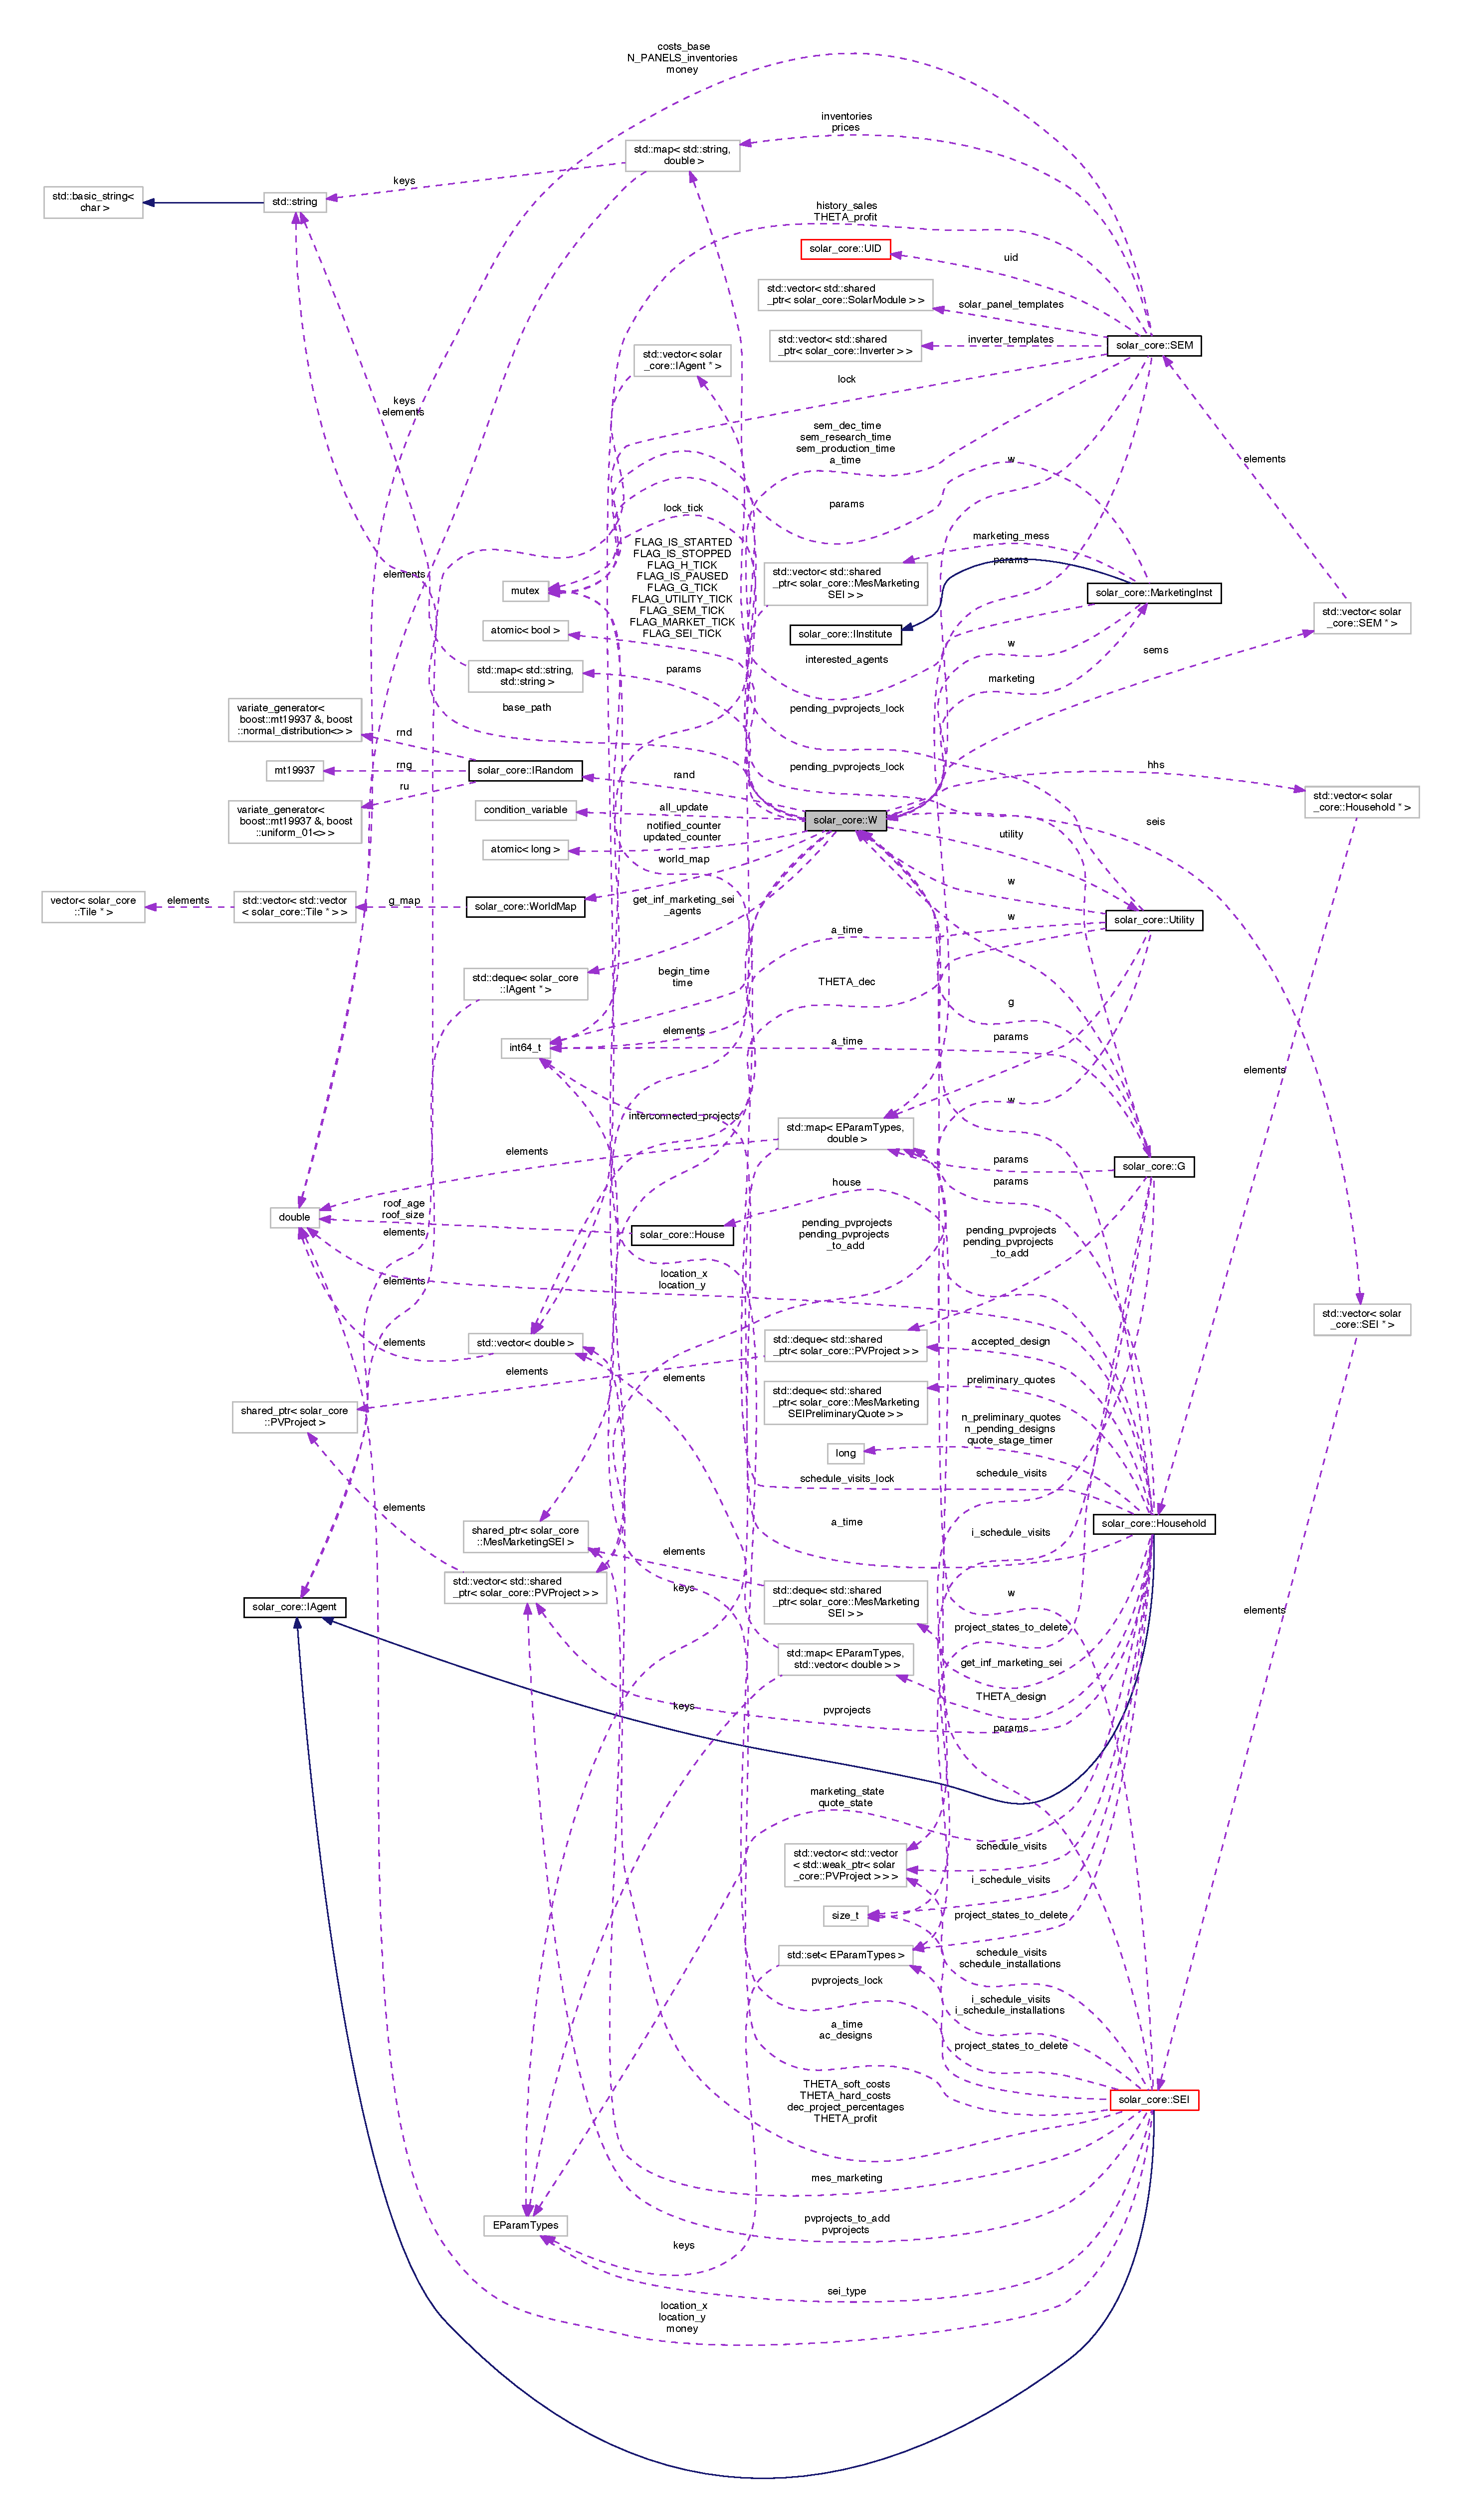
\includegraphics[height=550pt]{classsolar__core_1_1_w__coll__graph}
=======
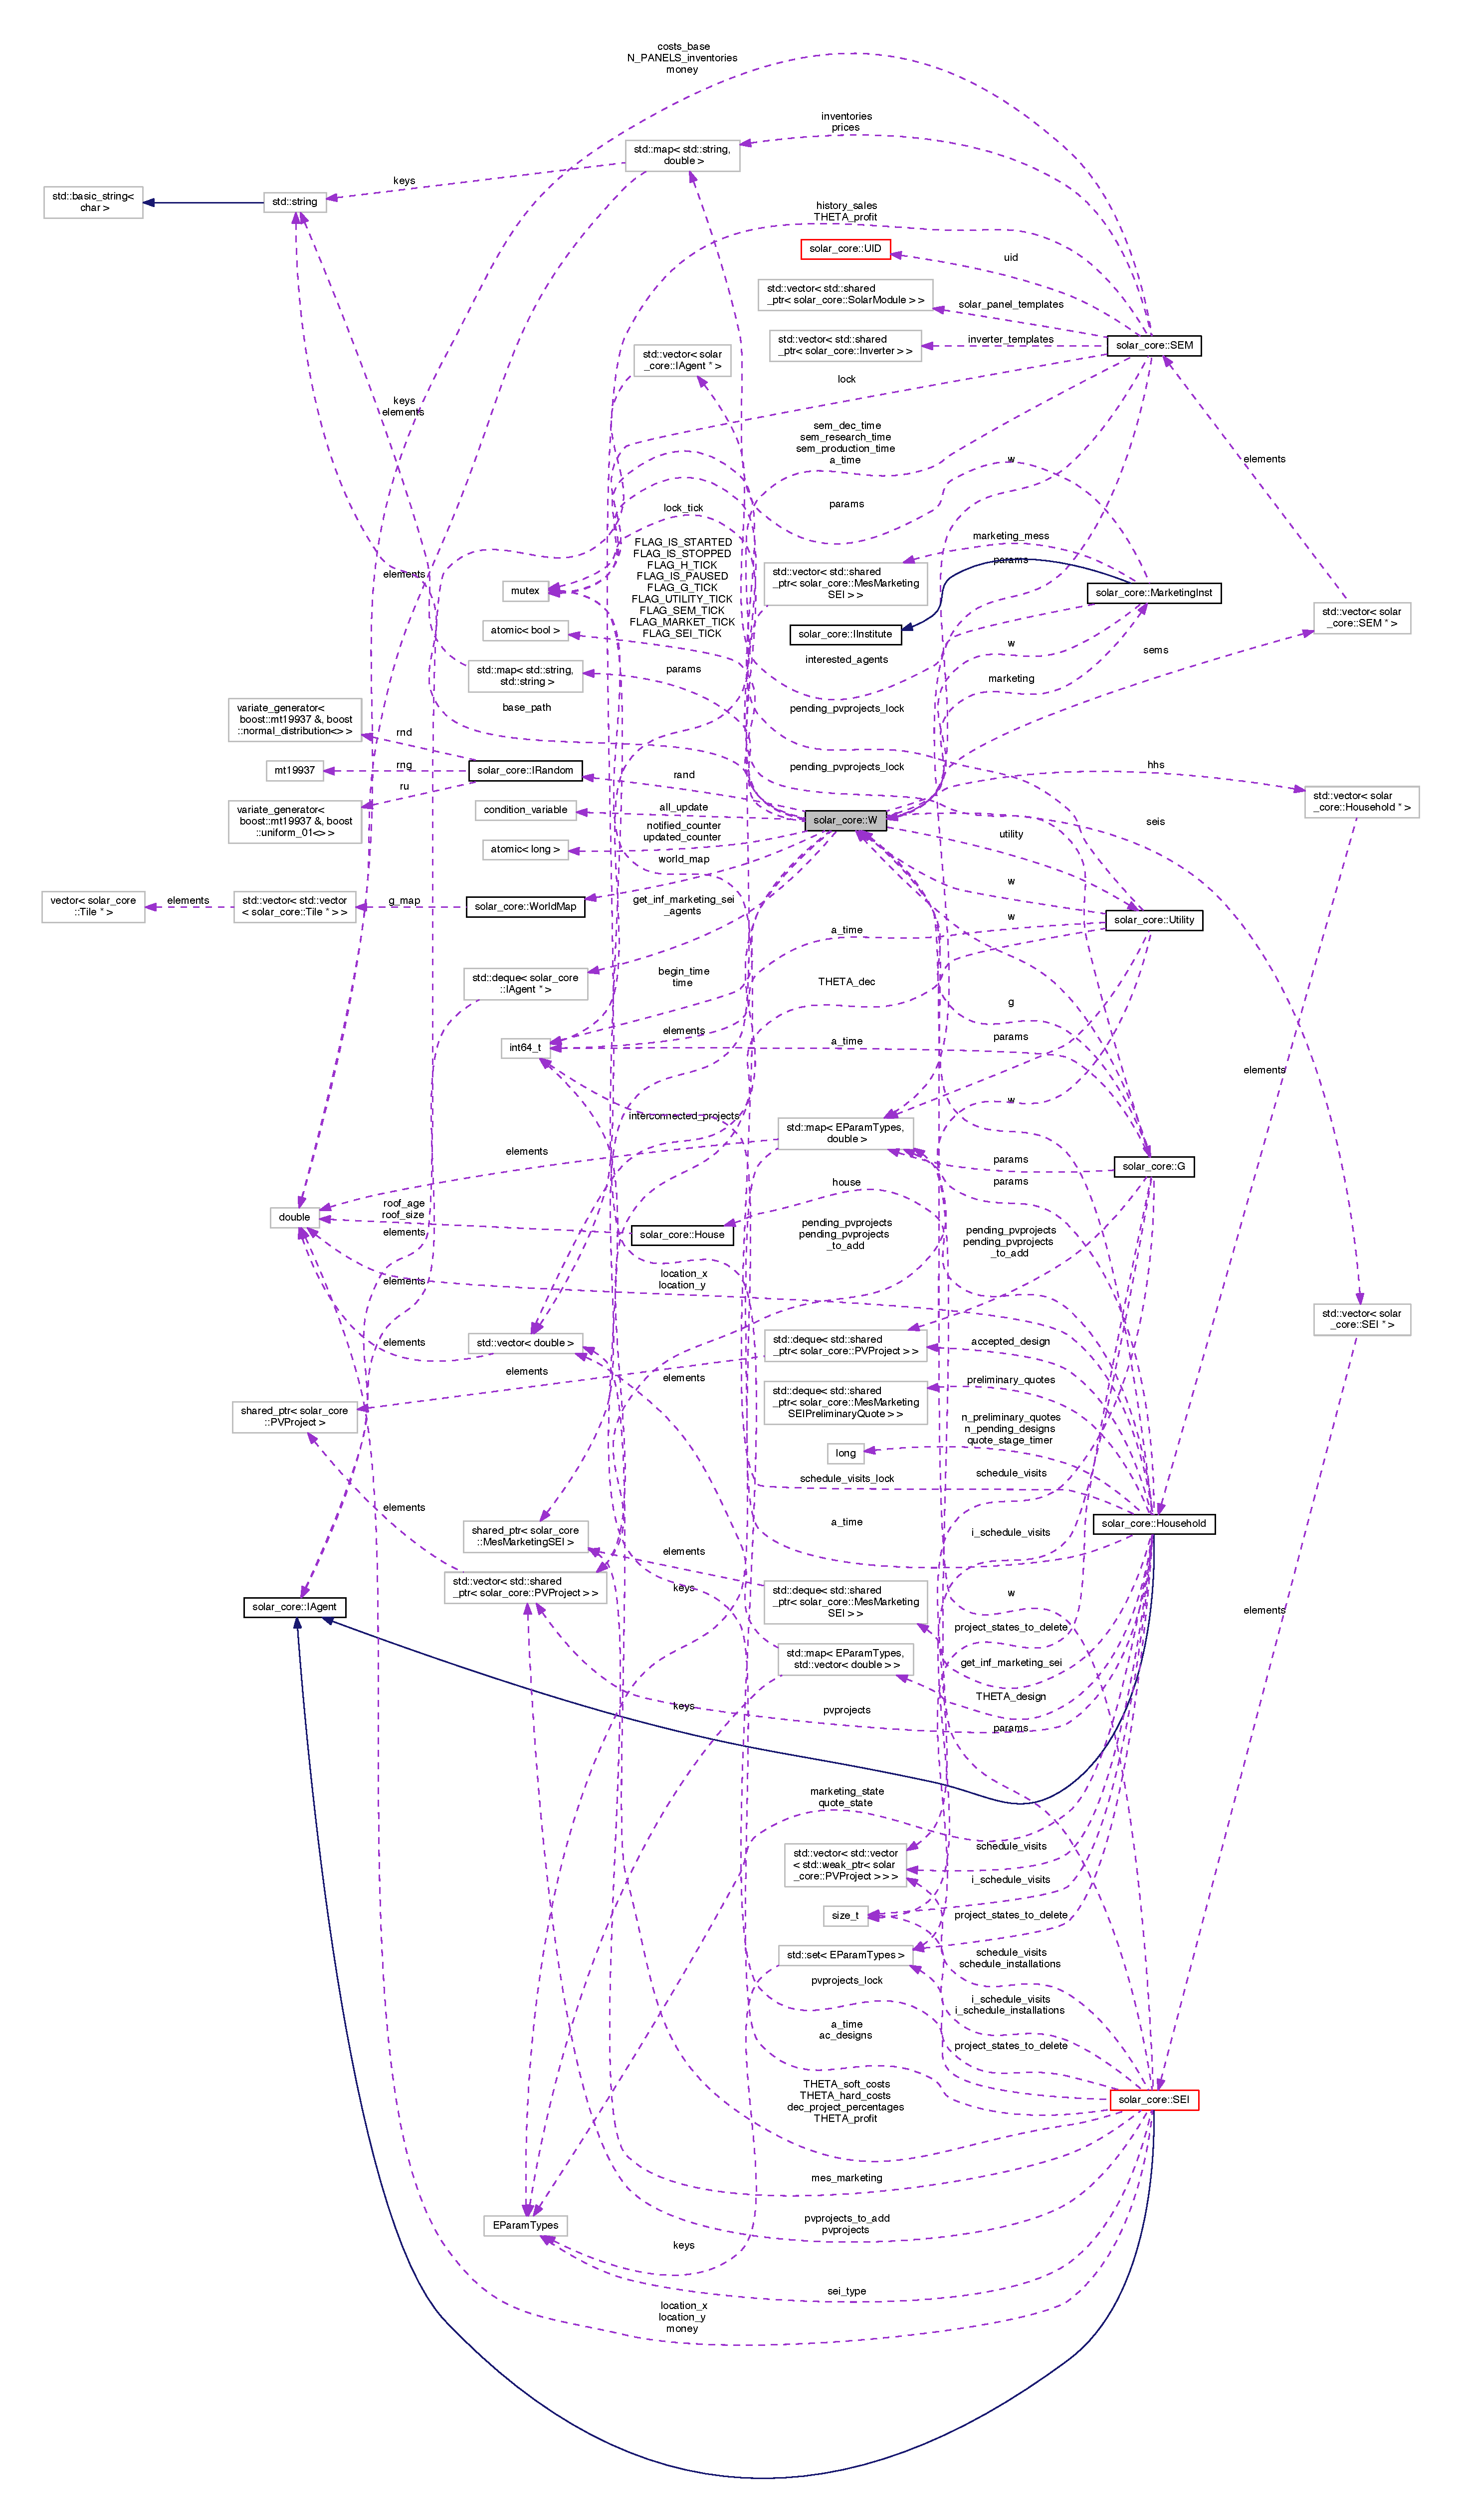
\includegraphics[width=350pt]{classsolar__core_1_1_w__coll__graph}
>>>>>>> 9fadf023062505cb443534457ab9d4d3cc1b7bfc
\end{center}
\end{figure}
\subsection*{Public Member Functions}
{\bf }\par
\begin{DoxyCompactItemize}
\item 
void \hyperlink{classsolar__core_1_1_w_a5e64e5a7ef41c07fddf7994cd3f2693e}{life} ()
\item 
void \hyperlink{classsolar__core_1_1_w_a08283dbea7c7f3fe8b7f094a96f73a78}{life\+\_\+hhs} ()
\item 
void \hyperlink{classsolar__core_1_1_w_a77b206056c9440059f7b78e1424b0921}{life\+\_\+seis} ()
<<<<<<< HEAD
\item 
void \hyperlink{classsolar__core_1_1_w_a655c14c2a3d10952ab1217eedd21443f}{life\+\_\+sems} ()
\item 
void \hyperlink{classsolar__core_1_1_w_ad08af315706bb42ab5dd68f41a90c978}{life\+\_\+gs} ()
\item 
void \hyperlink{classsolar__core_1_1_w_a03a16fe70a11b947735709cf0a0b277e}{life\+\_\+markets} ()
=======
>>>>>>> 9fadf023062505cb443534457ab9d4d3cc1b7bfc
\end{DoxyCompactItemize}

{\bf }\par
\begin{DoxyCompactItemize}
\item 
<<<<<<< HEAD
void \hyperlink{classsolar__core_1_1_w_a7fd073f0ebbf06378919f677bc28c2d1}{get\+\_\+state\+\_\+inf} (\hyperlink{classsolar__core_1_1_household}{Household} $\ast$agent\+\_\+, \hyperlink{namespacesolar__core_aa1147341e5ef7a40d68d1bd68e149362}{E\+Param\+Types} state\+\_\+)
\item 
void \hyperlink{classsolar__core_1_1_w_a1d99a46827c504a542ecda81b201a8f5}{get\+\_\+state\+\_\+inf\+\_\+installed\+\_\+project} (std\+::shared\+\_\+ptr$<$ \hyperlink{classsolar__core_1_1_p_v_project}{P\+V\+Project} $>$ project\+\_\+)
\item 
void \hyperlink{classsolar__core_1_1_w_a04252bc7247e71aa41798e98e42b6c15}{get\+\_\+state\+\_\+inf\+\_\+interconnected\+\_\+project} (std\+::shared\+\_\+ptr$<$ \hyperlink{classsolar__core_1_1_p_v_project}{P\+V\+Project} $>$ project\+\_\+)
=======
double \hyperlink{classsolar__core_1_1_w_a39001b1adeb816c80cb63637801c4b9c}{get\+\_\+solar\+\_\+radiation} (double location\+\_\+x, double location\+\_\+y) const 
\item 
double \hyperlink{classsolar__core_1_1_w_a7906874c5180d8114e1acba095ace3f5}{get\+\_\+permit\+\_\+difficulty} (double location\+\_\+x, double location\+\_\+y) const 
>>>>>>> 9fadf023062505cb443534457ab9d4d3cc1b7bfc
\end{DoxyCompactItemize}

\subsection*{Public Attributes}
{\bf }\par
\begin{DoxyCompactItemize}
\item 
std\+::atomic$<$ bool $>$ \hyperlink{classsolar__core_1_1_w_a9bb998c65a7427961de179f41e25daea}{F\+L\+A\+G\+\_\+\+I\+S\+\_\+\+S\+T\+O\+P\+P\+E\+D}
\item 
std\+::atomic$<$ bool $>$ \hyperlink{classsolar__core_1_1_w_a8456f88d45f2e8bf67eccd7f0c8d08fa}{F\+L\+A\+G\+\_\+\+I\+S\+\_\+\+S\+T\+A\+R\+T\+E\+D}
\item 
<<<<<<< HEAD
std\+::atomic$<$ bool $>$ \hyperlink{classsolar__core_1_1_w_a1c0ebdba727a7a5cbf322072ab5c9184}{F\+L\+A\+G\+\_\+\+I\+S\+\_\+\+P\+A\+U\+S\+E\+D}
\item 
=======
>>>>>>> 9fadf023062505cb443534457ab9d4d3cc1b7bfc
\hyperlink{namespacesolar__core_a4b5949d07259da6f8a20d12a30403e90}{Time\+Unit} \hyperlink{classsolar__core_1_1_w_ae96b30122adc9fae8fc2f209a4c89b0a}{time}
\item 
\hyperlink{namespacesolar__core_a4b5949d07259da6f8a20d12a30403e90}{Time\+Unit} \hyperlink{classsolar__core_1_1_w_aec1b9014ad296dc9b8b132ba9b67c08a}{begin\+\_\+time} = 0
\item 
std\+::mutex \hyperlink{classsolar__core_1_1_w_a56ba20ee51f5db7288e55bb65f12511b}{lock\+\_\+tick}
\item 
std\+::condition\+\_\+variable \hyperlink{classsolar__core_1_1_w_aa6cba0dba8a566978e51fb4204aac4b9}{all\+\_\+update}
\item 
std\+::atomic$<$ long $>$ \hyperlink{classsolar__core_1_1_w_a775d817c6117b462571c3fca62fe0c86}{updated\+\_\+counter}
\item 
std\+::atomic$<$ long $>$ \hyperlink{classsolar__core_1_1_w_afee32d515534826a60ddf12936f85a3d}{notified\+\_\+counter}
\item 
std\+::atomic$<$ bool $>$ \hyperlink{classsolar__core_1_1_w_a65d2047e574ed6201a8e21ec1ba1bec4}{F\+L\+A\+G\+\_\+\+S\+E\+I\+\_\+\+T\+I\+C\+K}
\item 
std\+::atomic$<$ bool $>$ \hyperlink{classsolar__core_1_1_w_a4cd32940e21bfc20919cc2d4447d66d3}{F\+L\+A\+G\+\_\+\+H\+\_\+\+T\+I\+C\+K}
\item 
std\+::atomic$<$ bool $>$ \hyperlink{classsolar__core_1_1_w_aae63ce0d440f2c8d475d6eeafac58238}{F\+L\+A\+G\+\_\+\+G\+\_\+\+T\+I\+C\+K}
\item 
<<<<<<< HEAD
std\+::atomic$<$ bool $>$ \hyperlink{classsolar__core_1_1_w_a7aa8b882244539e098e45207045d7d88}{F\+L\+A\+G\+\_\+\+M\+A\+R\+K\+E\+T\+\_\+\+T\+I\+C\+K}
\item 
std\+::atomic$<$ bool $>$ \hyperlink{classsolar__core_1_1_w_ae383b7a595cb28d52aa747fc7e5bb619}{F\+L\+A\+G\+\_\+\+S\+E\+M\+\_\+\+T\+I\+C\+K}
\item 
\hyperlink{classsolar__core_1_1_i_random}{I\+Random} $\ast$ \hyperlink{classsolar__core_1_1_w_aa60afb55012cd72e304ac2c133e5a245}{rand} = nullptr
=======
std\+::atomic$<$ bool $>$ \hyperlink{classsolar__core_1_1_w_ae383b7a595cb28d52aa747fc7e5bb619}{F\+L\+A\+G\+\_\+\+S\+E\+M\+\_\+\+T\+I\+C\+K}
>>>>>>> 9fadf023062505cb443534457ab9d4d3cc1b7bfc
\end{DoxyCompactItemize}

{\bf }\par
\begin{DoxyCompactItemize}
\item 
\hyperlink{classsolar__core_1_1_g}{G} $\ast$ \hyperlink{classsolar__core_1_1_w_a9e50ef0da579cdfc3da22c16a492bc44}{g}
<<<<<<< HEAD
\item 
\hyperlink{classsolar__core_1_1_marketing_inst}{Marketing\+Inst} $\ast$ \hyperlink{classsolar__core_1_1_w_a93f277fb3a9d9e7b1e911c6a494c8ec8}{marketing}
\item 
\hyperlink{classsolar__core_1_1_utility}{Utility} $\ast$ \hyperlink{classsolar__core_1_1_w_a6d6fa51d4bdc40dac8b76aa4967030b5}{utility}
=======
>>>>>>> 9fadf023062505cb443534457ab9d4d3cc1b7bfc
\end{DoxyCompactItemize}

\subsection*{Protected Attributes}
\begin{DoxyCompactItemize}
\item 
std\+::deque$<$ \hyperlink{classsolar__core_1_1_i_agent}{I\+Agent} $\ast$ $>$ \hyperlink{classsolar__core_1_1_w_a81b5469757f203c9619ff69323ac0f77}{get\+\_\+inf\+\_\+marketing\+\_\+sei\+\_\+agents}
\item 
std\+::vector$<$ \hyperlink{classsolar__core_1_1_household}{Household} $\ast$ $>$ \hyperlink{classsolar__core_1_1_w_a17c012ff8b17890ed33923cec6d87be3}{hhs}
\item 
std\+::vector$<$ \hyperlink{classsolar__core_1_1_s_e_i}{S\+E\+I} $\ast$ $>$ \hyperlink{classsolar__core_1_1_w_a311baa30390494ae8e79f26e372e716d}{seis}
\item 
<<<<<<< HEAD
std\+::vector$<$ \hyperlink{classsolar__core_1_1_s_e_m}{S\+E\+M} $\ast$ $>$ \hyperlink{classsolar__core_1_1_w_ab6349cbc751747a05618dad4ebb1b726}{sems}
\item 
std\+::map$<$ std\+::string, std\+::string $>$ \hyperlink{classsolar__core_1_1_w_a0d06bc7242f8b3958986118eb217583f}{params}
\item 
std\+::vector$<$ std\+::shared\+\_\+ptr$<$ \hyperlink{classsolar__core_1_1_p_v_project}{P\+V\+Project} $>$ $>$ \hyperlink{classsolar__core_1_1_w_a1d35d6501eef6d673bd2b28e2c1724c4}{interconnected\+\_\+projects}
\end{DoxyCompactItemize}
\subsection*{Friends}
\begin{DoxyCompactItemize}
\item 
class \hyperlink{classsolar__core_1_1_w_ac01e54f17f927af30196b551d235d7ba}{Marketing\+Inst}
\item 
class \hyperlink{classsolar__core_1_1_w_a8f3690c82c493af3a66f999410fe891d}{solar\+\_\+ui\+::\+U\+I}
=======
std\+::vector$<$ S\+E\+M $\ast$ $>$ \hyperlink{classsolar__core_1_1_w_ab6349cbc751747a05618dad4ebb1b726}{sems}
\item 
std\+::map$<$ std\+::string, std\+::string $>$ \hyperlink{classsolar__core_1_1_w_a0d06bc7242f8b3958986118eb217583f}{params}
\item 
\hyperlink{classsolar__core_1_1_world_map}{World\+Map} $\ast$ \hyperlink{classsolar__core_1_1_w_a8ed6f1aa7fd4ef2c3488147b38a670b7}{world\+\_\+map}
>>>>>>> 9fadf023062505cb443534457ab9d4d3cc1b7bfc
\end{DoxyCompactItemize}
\begin{DoxyCompactItemize}
\item 
std\+::string \hyperlink{classsolar__core_1_1_w_acf6e7dd195573ba04b406cde2e5b80fb}{base\+\_\+path}
\item 
<<<<<<< HEAD
\hyperlink{classsolar__core_1_1_w_a969ad4de57020878a91873868c9bdb45}{W} (std\+::string path\+\_\+, \hyperlink{classsolar__core_1_1_helper_w}{Helper\+W} $\ast$w\+\_\+, std\+::string mode\+\_\+=\char`\"{}N\+E\+W\char`\"{})
\item 
void \hyperlink{classsolar__core_1_1_w_af58a19a39fb9fb34258803c613924613}{init} ()
\item 
virtual void \hyperlink{classsolar__core_1_1_w_a0b92657c681579dacc29821f41650541}{create\+\_\+seis} (\hyperlink{namespacesolar__core_adeda2737d6938c190eb774a5b2495045}{Property\+Tree} \&pt\+\_\+, std\+::string mode\+\_\+, long N\+\_\+\+S\+E\+I, long N\+\_\+\+S\+E\+I\+Large, boost\+::variate\+\_\+generator$<$ boost\+::mt19937 \&, boost\+::uniform\+\_\+int$<$ uint64\+\_\+t $>$$>$ \&rng\+\_\+location\+\_\+x, boost\+::variate\+\_\+generator$<$ boost\+::mt19937 \&, boost\+::uniform\+\_\+int$<$ uint64\+\_\+t $>$$>$ \&rng\+\_\+location\+\_\+y)
\end{DoxyCompactItemize}
\begin{DoxyCompactItemize}
\item 
\hyperlink{classsolar__core_1_1_world_map}{World\+Map} $\ast$ \hyperlink{classsolar__core_1_1_w_a8ed6f1aa7fd4ef2c3488147b38a670b7}{world\+\_\+map}
\item 
double \hyperlink{classsolar__core_1_1_w_af3adfe566e6db1a7f7df18aa7df22c25}{get\+\_\+solar\+\_\+irradiation} (double location\+\_\+x, double location\+\_\+y) const 
\item 
double \hyperlink{classsolar__core_1_1_w_a7906874c5180d8114e1acba095ace3f5}{get\+\_\+permit\+\_\+difficulty} (double location\+\_\+x, double location\+\_\+y) const 
=======
\hyperlink{classsolar__core_1_1_w_aa252edac9babf33b41e22a816648a9a5}{W} (std\+::string path\+\_\+, std\+::string mode\+\_\+=\char`\"{}N\+E\+W\char`\"{})
>>>>>>> 9fadf023062505cb443534457ab9d4d3cc1b7bfc
\end{DoxyCompactItemize}


\subsection{Detailed Description}


<<<<<<< HEAD
Definition at line 42 of file W.\+h.
=======
Definition at line 30 of file W.\+h.
>>>>>>> 9fadf023062505cb443534457ab9d4d3cc1b7bfc



\subsection{Constructor \& Destructor Documentation}
<<<<<<< HEAD
\hypertarget{classsolar__core_1_1_w_a969ad4de57020878a91873868c9bdb45}{}\index{solar\+\_\+core\+::\+W@{solar\+\_\+core\+::\+W}!W@{W}}
=======
\hypertarget{classsolar__core_1_1_w_aa252edac9babf33b41e22a816648a9a5}{}\index{solar\+\_\+core\+::\+W@{solar\+\_\+core\+::\+W}!W@{W}}
>>>>>>> 9fadf023062505cb443534457ab9d4d3cc1b7bfc
\index{W@{W}!solar\+\_\+core\+::\+W@{solar\+\_\+core\+::\+W}}
\subsubsection[{W}]{\setlength{\rightskip}{0pt plus 5cm}W\+::\+W (
\begin{DoxyParamCaption}
\item[{std\+::string}]{path\+\_\+, }
<<<<<<< HEAD
\item[{{\bf Helper\+W} $\ast$}]{helper\+\_\+, }
\item[{std\+::string}]{mode\+\_\+ = {\ttfamily \char`\"{}NEW\char`\"{}}}
\end{DoxyParamCaption}
)}\label{classsolar__core_1_1_w_a969ad4de57020878a91873868c9bdb45}
=======
\item[{std\+::string}]{mode\+\_\+ = {\ttfamily \char`\"{}NEW\char`\"{}}}
\end{DoxyParamCaption}
)}\label{classsolar__core_1_1_w_aa252edac9babf33b41e22a816648a9a5}
>>>>>>> 9fadf023062505cb443534457ab9d4d3cc1b7bfc
Section with initialization and serialization code.

Multiple step initialization from the project file. Keep structure of a project file simple, all parameters in one file.

<<<<<<< HEAD
\begin{DoxyRefDesc}{Dev\+Stage2}
\item[\hyperlink{_dev_stage2__DevStage2000029}{Dev\+Stage2}]\+: serialization\+: choose custom/binary/to database. For now think that cereal will be emough, with saving to .json. All agents of the same type will be saved in the same file. Loading also from .json with simple structure.\end{DoxyRefDesc}


Assume that world is created from scratch \begin{DoxyRefDesc}{Dev\+Stage2}
\item[\hyperlink{_dev_stage2__DevStage2000028}{Dev\+Stage2}]each sem will pick initial templates by name? -\/ could make it base creation mode \end{DoxyRefDesc}


Definition at line 40 of file W.\+cpp.
=======
\+: serialization\+: choose custom/binary/to database. For now think that cereal will be emough, with saving to .json. All agents of the same type will be saved in the same file. Loading also from .json with simple structure.

Assume that world is created from scratch 

Definition at line 35 of file W.\+cpp.
>>>>>>> 9fadf023062505cb443534457ab9d4d3cc1b7bfc



Here is the call graph for this function\+:
\nopagebreak
\begin{figure}[H]
\begin{center}
\leavevmode
<<<<<<< HEAD
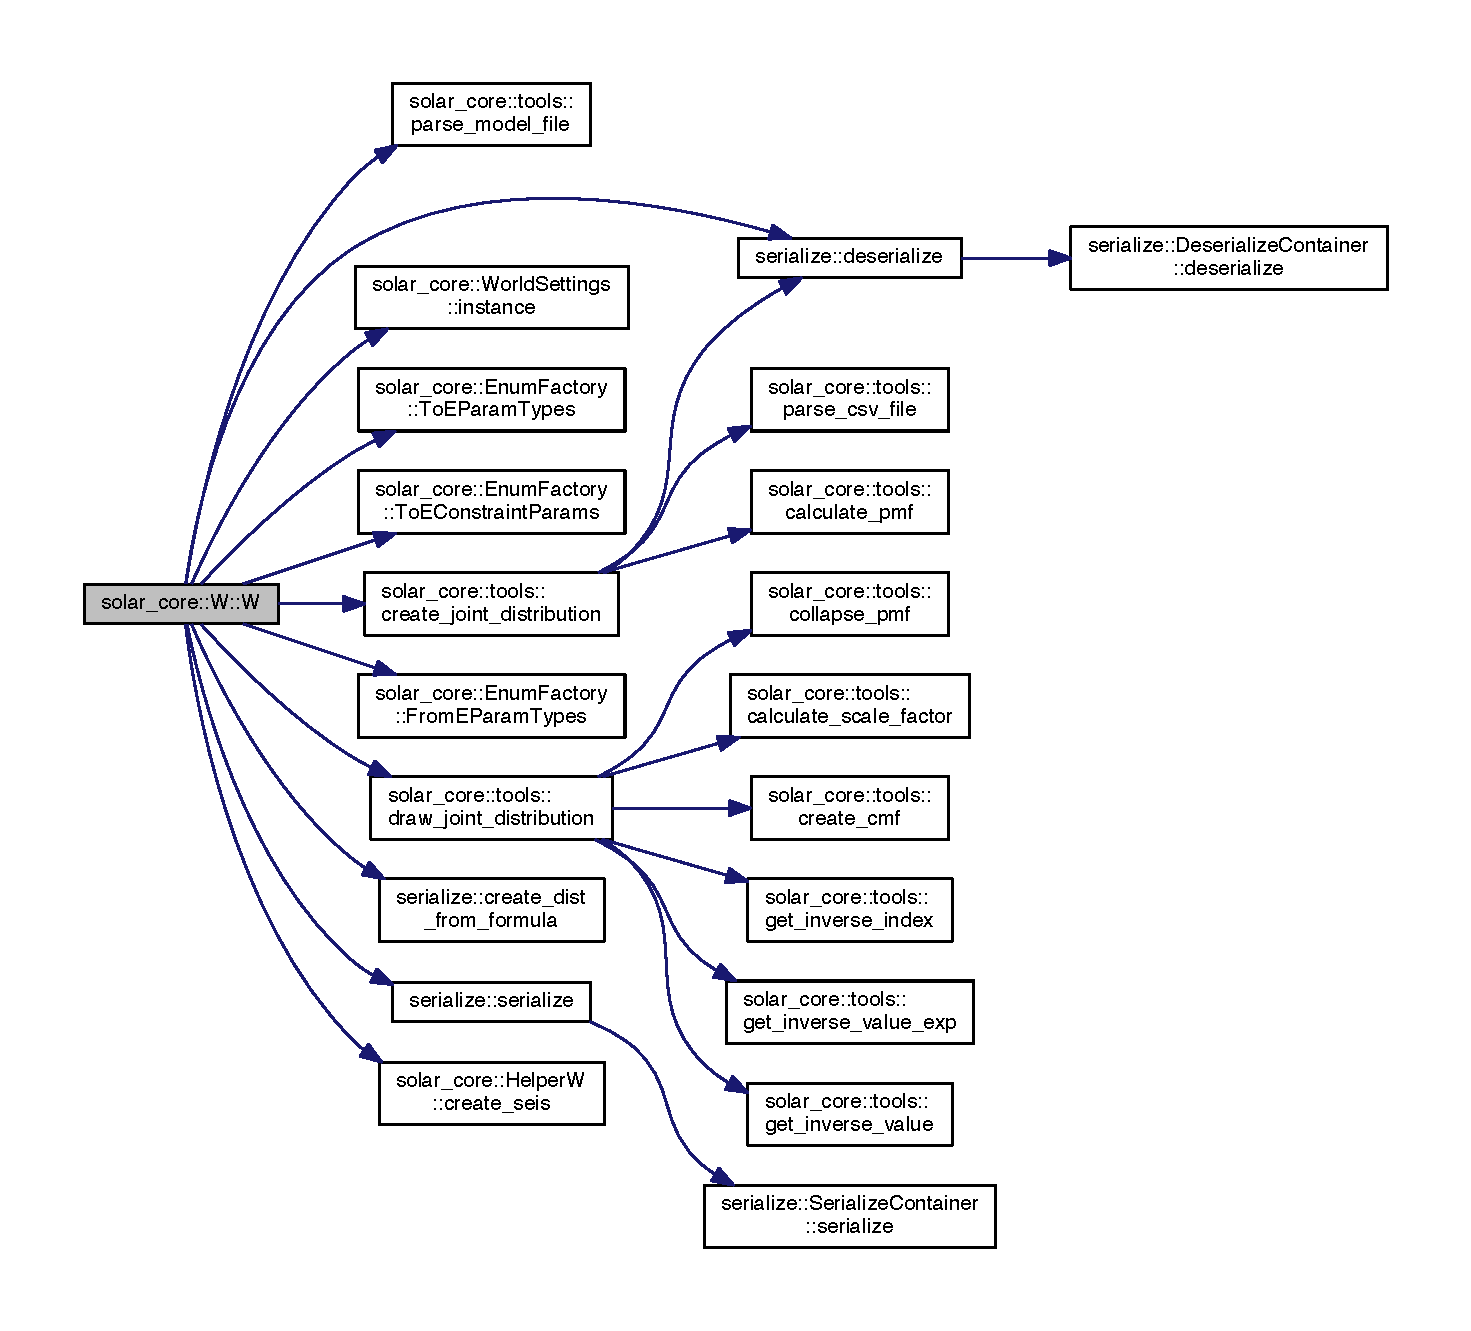
\includegraphics[width=350pt]{classsolar__core_1_1_w_a969ad4de57020878a91873868c9bdb45_cgraph}
=======
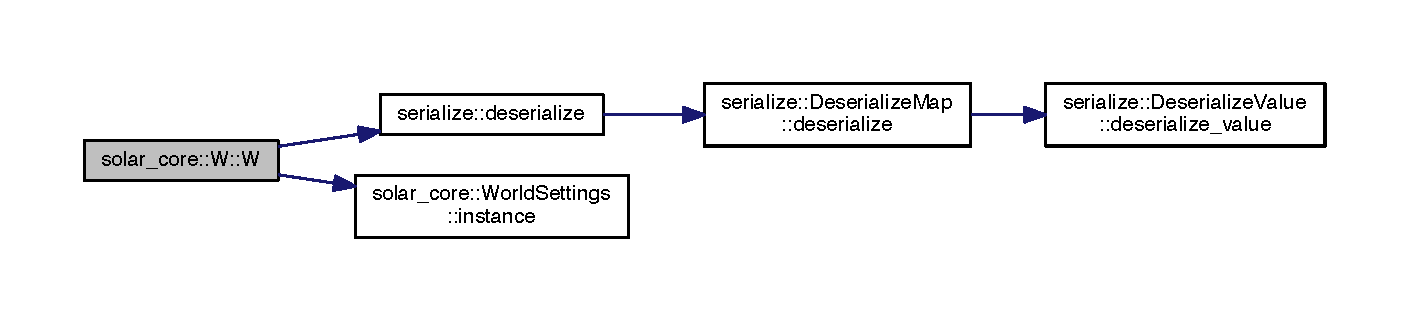
\includegraphics[width=350pt]{classsolar__core_1_1_w_aa252edac9babf33b41e22a816648a9a5_cgraph}
>>>>>>> 9fadf023062505cb443534457ab9d4d3cc1b7bfc
\end{center}
\end{figure}




\subsection{Member Function Documentation}
<<<<<<< HEAD
\hypertarget{classsolar__core_1_1_w_a0b92657c681579dacc29821f41650541}{}\index{solar\+\_\+core\+::\+W@{solar\+\_\+core\+::\+W}!create\+\_\+seis@{create\+\_\+seis}}
\index{create\+\_\+seis@{create\+\_\+seis}!solar\+\_\+core\+::\+W@{solar\+\_\+core\+::\+W}}
\subsubsection[{create\+\_\+seis}]{\setlength{\rightskip}{0pt plus 5cm}void W\+::create\+\_\+seis (
\begin{DoxyParamCaption}
\item[{{\bf Property\+Tree} \&}]{pt\+\_\+, }
\item[{std\+::string}]{mode\+\_\+, }
\item[{long}]{N\+\_\+\+S\+E\+I, }
\item[{long}]{N\+\_\+\+S\+E\+I\+Large, }
\item[{boost\+::variate\+\_\+generator$<$ boost\+::mt19937 \&, boost\+::uniform\+\_\+int$<$ uint64\+\_\+t $>$$>$ \&}]{rng\+\_\+location\+\_\+x, }
\item[{boost\+::variate\+\_\+generator$<$ boost\+::mt19937 \&, boost\+::uniform\+\_\+int$<$ uint64\+\_\+t $>$$>$ \&}]{rng\+\_\+location\+\_\+y}
\end{DoxyParamCaption}
)\hspace{0.3cm}{\ttfamily [virtual]}}\label{classsolar__core_1_1_w_a0b92657c681579dacc29821f41650541}


Definition at line 326 of file W.\+cpp.



Here is the call graph for this function\+:
\nopagebreak
\begin{figure}[H]
\begin{center}
\leavevmode
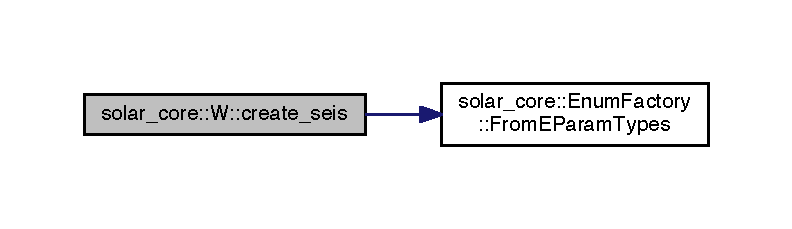
\includegraphics[width=350pt]{classsolar__core_1_1_w_a0b92657c681579dacc29821f41650541_cgraph}
\end{center}
\end{figure}


=======
>>>>>>> 9fadf023062505cb443534457ab9d4d3cc1b7bfc
\hypertarget{classsolar__core_1_1_w_a7906874c5180d8114e1acba095ace3f5}{}\index{solar\+\_\+core\+::\+W@{solar\+\_\+core\+::\+W}!get\+\_\+permit\+\_\+difficulty@{get\+\_\+permit\+\_\+difficulty}}
\index{get\+\_\+permit\+\_\+difficulty@{get\+\_\+permit\+\_\+difficulty}!solar\+\_\+core\+::\+W@{solar\+\_\+core\+::\+W}}
\subsubsection[{get\+\_\+permit\+\_\+difficulty}]{\setlength{\rightskip}{0pt plus 5cm}double W\+::get\+\_\+permit\+\_\+difficulty (
\begin{DoxyParamCaption}
\item[{double}]{location\+\_\+x, }
\item[{double}]{location\+\_\+y}
\end{DoxyParamCaption}
) const}\label{classsolar__core_1_1_w_a7906874c5180d8114e1acba095ace3f5}
returns permit difficulty 

<<<<<<< HEAD
Definition at line 625 of file W.\+cpp.
=======
Definition at line 206 of file W.\+cpp.
>>>>>>> 9fadf023062505cb443534457ab9d4d3cc1b7bfc



Here is the caller graph for this function\+:
\nopagebreak
\begin{figure}[H]
\begin{center}
\leavevmode
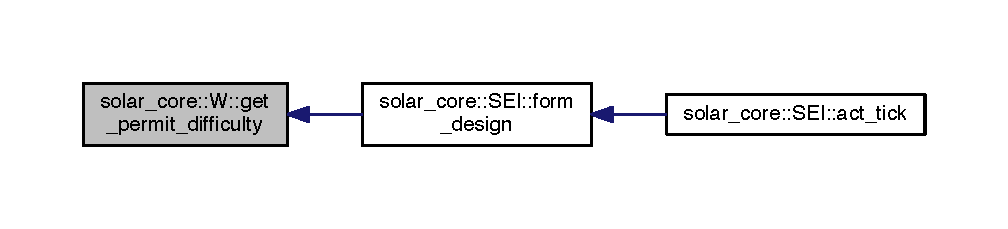
\includegraphics[width=350pt]{classsolar__core_1_1_w_a7906874c5180d8114e1acba095ace3f5_icgraph}
\end{center}
\end{figure}


<<<<<<< HEAD
\hypertarget{classsolar__core_1_1_w_af3adfe566e6db1a7f7df18aa7df22c25}{}\index{solar\+\_\+core\+::\+W@{solar\+\_\+core\+::\+W}!get\+\_\+solar\+\_\+irradiation@{get\+\_\+solar\+\_\+irradiation}}
\index{get\+\_\+solar\+\_\+irradiation@{get\+\_\+solar\+\_\+irradiation}!solar\+\_\+core\+::\+W@{solar\+\_\+core\+::\+W}}
\subsubsection[{get\+\_\+solar\+\_\+irradiation}]{\setlength{\rightskip}{0pt plus 5cm}double W\+::get\+\_\+solar\+\_\+irradiation (
=======
\hypertarget{classsolar__core_1_1_w_a39001b1adeb816c80cb63637801c4b9c}{}\index{solar\+\_\+core\+::\+W@{solar\+\_\+core\+::\+W}!get\+\_\+solar\+\_\+radiation@{get\+\_\+solar\+\_\+radiation}}
\index{get\+\_\+solar\+\_\+radiation@{get\+\_\+solar\+\_\+radiation}!solar\+\_\+core\+::\+W@{solar\+\_\+core\+::\+W}}
\subsubsection[{get\+\_\+solar\+\_\+radiation}]{\setlength{\rightskip}{0pt plus 5cm}double W\+::get\+\_\+solar\+\_\+radiation (
>>>>>>> 9fadf023062505cb443534457ab9d4d3cc1b7bfc
\begin{DoxyParamCaption}
\item[{double}]{location\+\_\+x, }
\item[{double}]{location\+\_\+y}
\end{DoxyParamCaption}
<<<<<<< HEAD
) const}\label{classsolar__core_1_1_w_af3adfe566e6db1a7f7df18aa7df22c25}
Interactions on geographyreturns estimated amount of solar irradiation for the tile 

Definition at line 619 of file W.\+cpp.



Here is the caller graph for this function\+:
\nopagebreak
\begin{figure}[H]
\begin{center}
\leavevmode
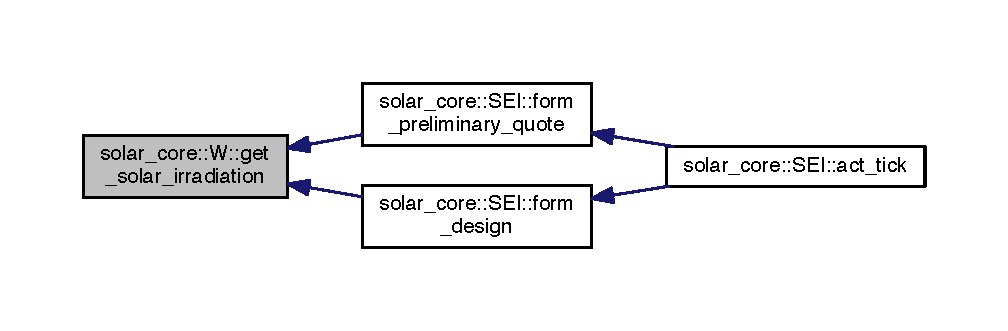
\includegraphics[width=350pt]{classsolar__core_1_1_w_af3adfe566e6db1a7f7df18aa7df22c25_icgraph}
\end{center}
\end{figure}


\hypertarget{classsolar__core_1_1_w_a7fd073f0ebbf06378919f677bc28c2d1}{}\index{solar\+\_\+core\+::\+W@{solar\+\_\+core\+::\+W}!get\+\_\+state\+\_\+inf@{get\+\_\+state\+\_\+inf}}
\index{get\+\_\+state\+\_\+inf@{get\+\_\+state\+\_\+inf}!solar\+\_\+core\+::\+W@{solar\+\_\+core\+::\+W}}
\subsubsection[{get\+\_\+state\+\_\+inf}]{\setlength{\rightskip}{0pt plus 5cm}void W\+::get\+\_\+state\+\_\+inf (
\begin{DoxyParamCaption}
\item[{{\bf Household} $\ast$}]{agent\+\_\+, }
\item[{{\bf E\+Param\+Types}}]{state\+\_\+}
\end{DoxyParamCaption}
)}\label{classsolar__core_1_1_w_a7fd073f0ebbf06378919f677bc28c2d1}
Interactions with other agentsgets information about state change from agent 

Definition at line 632 of file W.\+cpp.
=======
) const}\label{classsolar__core_1_1_w_a39001b1adeb816c80cb63637801c4b9c}
Interactions on geographyreturns estimated amount of solar radiation for the tile 

Definition at line 200 of file W.\+cpp.
>>>>>>> 9fadf023062505cb443534457ab9d4d3cc1b7bfc



Here is the caller graph for this function\+:
\nopagebreak
\begin{figure}[H]
\begin{center}
\leavevmode
<<<<<<< HEAD
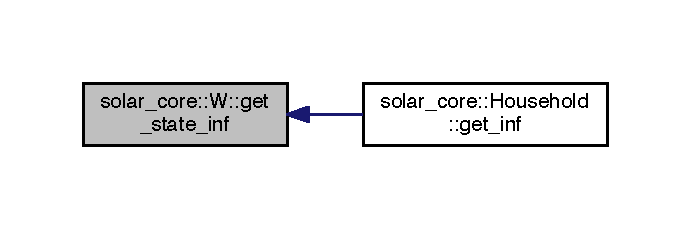
\includegraphics[width=332pt]{classsolar__core_1_1_w_a7fd073f0ebbf06378919f677bc28c2d1_icgraph}
\end{center}
\end{figure}


\hypertarget{classsolar__core_1_1_w_a1d99a46827c504a542ecda81b201a8f5}{}\index{solar\+\_\+core\+::\+W@{solar\+\_\+core\+::\+W}!get\+\_\+state\+\_\+inf\+\_\+installed\+\_\+project@{get\+\_\+state\+\_\+inf\+\_\+installed\+\_\+project}}
\index{get\+\_\+state\+\_\+inf\+\_\+installed\+\_\+project@{get\+\_\+state\+\_\+inf\+\_\+installed\+\_\+project}!solar\+\_\+core\+::\+W@{solar\+\_\+core\+::\+W}}
\subsubsection[{get\+\_\+state\+\_\+inf\+\_\+installed\+\_\+project}]{\setlength{\rightskip}{0pt plus 5cm}void W\+::get\+\_\+state\+\_\+inf\+\_\+installed\+\_\+project (
\begin{DoxyParamCaption}
\item[{std\+::shared\+\_\+ptr$<$ {\bf P\+V\+Project} $>$}]{project\+\_\+}
\end{DoxyParamCaption}
)}\label{classsolar__core_1_1_w_a1d99a46827c504a542ecda81b201a8f5}
is called when project is finished to record it 

Definition at line 639 of file W.\+cpp.



Here is the caller graph for this function\+:
\nopagebreak
\begin{figure}[H]
\begin{center}
\leavevmode
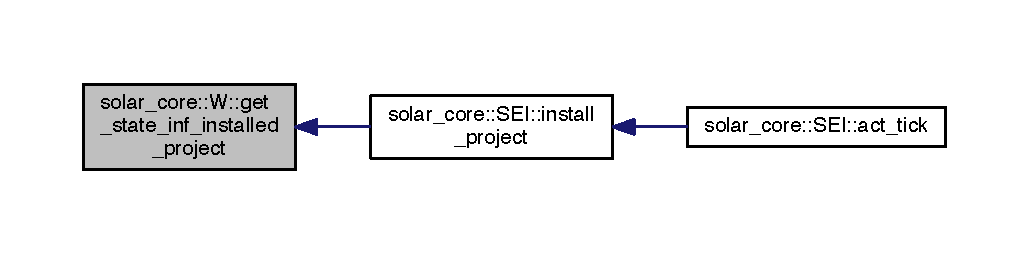
\includegraphics[width=350pt]{classsolar__core_1_1_w_a1d99a46827c504a542ecda81b201a8f5_icgraph}
\end{center}
\end{figure}


\hypertarget{classsolar__core_1_1_w_a04252bc7247e71aa41798e98e42b6c15}{}\index{solar\+\_\+core\+::\+W@{solar\+\_\+core\+::\+W}!get\+\_\+state\+\_\+inf\+\_\+interconnected\+\_\+project@{get\+\_\+state\+\_\+inf\+\_\+interconnected\+\_\+project}}
\index{get\+\_\+state\+\_\+inf\+\_\+interconnected\+\_\+project@{get\+\_\+state\+\_\+inf\+\_\+interconnected\+\_\+project}!solar\+\_\+core\+::\+W@{solar\+\_\+core\+::\+W}}
\subsubsection[{get\+\_\+state\+\_\+inf\+\_\+interconnected\+\_\+project}]{\setlength{\rightskip}{0pt plus 5cm}void W\+::get\+\_\+state\+\_\+inf\+\_\+interconnected\+\_\+project (
\begin{DoxyParamCaption}
\item[{std\+::shared\+\_\+ptr$<$ {\bf P\+V\+Project} $>$}]{project\+\_\+}
\end{DoxyParamCaption}
)}\label{classsolar__core_1_1_w_a04252bc7247e71aa41798e98e42b6c15}
is called when project is interconnected to record it 

Definition at line 646 of file W.\+cpp.



Here is the caller graph for this function\+:
\nopagebreak
\begin{figure}[H]
\begin{center}
\leavevmode
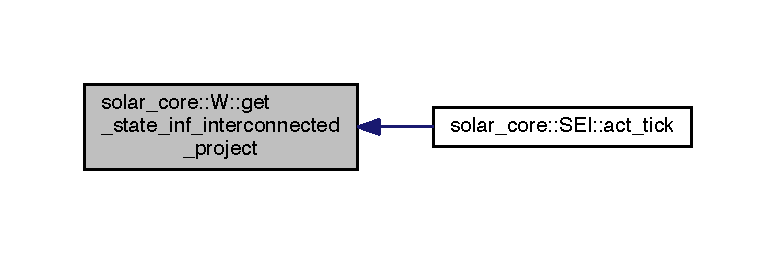
\includegraphics[width=350pt]{classsolar__core_1_1_w_a04252bc7247e71aa41798e98e42b6c15_icgraph}
\end{center}
\end{figure}


\hypertarget{classsolar__core_1_1_w_af58a19a39fb9fb34258803c613924613}{}\index{solar\+\_\+core\+::\+W@{solar\+\_\+core\+::\+W}!init@{init}}
\index{init@{init}!solar\+\_\+core\+::\+W@{solar\+\_\+core\+::\+W}}
\subsubsection[{init}]{\setlength{\rightskip}{0pt plus 5cm}void W\+::init (
\begin{DoxyParamCaption}
{}
\end{DoxyParamCaption}
)}\label{classsolar__core_1_1_w_af58a19a39fb9fb34258803c613924613}


Definition at line 367 of file W.\+cpp.



Here is the call graph for this function\+:
\nopagebreak
\begin{figure}[H]
\begin{center}
\leavevmode
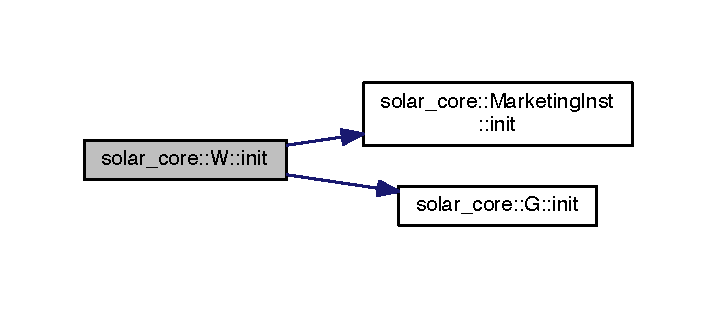
\includegraphics[width=344pt]{classsolar__core_1_1_w_af58a19a39fb9fb34258803c613924613_cgraph}
=======
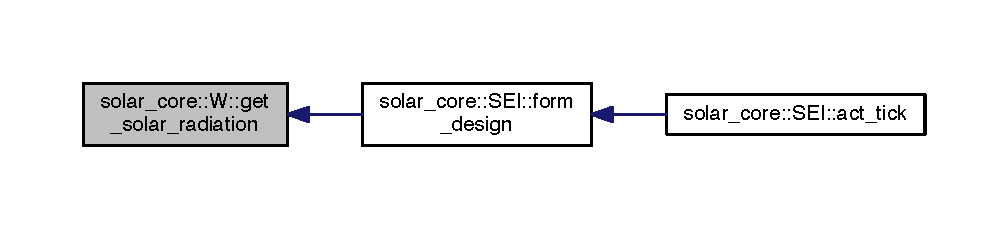
\includegraphics[width=350pt]{classsolar__core_1_1_w_a39001b1adeb816c80cb63637801c4b9c_icgraph}
>>>>>>> 9fadf023062505cb443534457ab9d4d3cc1b7bfc
\end{center}
\end{figure}


\hypertarget{classsolar__core_1_1_w_a5e64e5a7ef41c07fddf7994cd3f2693e}{}\index{solar\+\_\+core\+::\+W@{solar\+\_\+core\+::\+W}!life@{life}}
\index{life@{life}!solar\+\_\+core\+::\+W@{solar\+\_\+core\+::\+W}}
\subsubsection[{life}]{\setlength{\rightskip}{0pt plus 5cm}void W\+::life (
\begin{DoxyParamCaption}
{}
\end{DoxyParamCaption}
)}\label{classsolar__core_1_1_w_a5e64e5a7ef41c07fddf7994cd3f2693e}
Section with main loopgeneral loop 

<<<<<<< HEAD
Definition at line 400 of file W.\+cpp.

\hypertarget{classsolar__core_1_1_w_ad08af315706bb42ab5dd68f41a90c978}{}\index{solar\+\_\+core\+::\+W@{solar\+\_\+core\+::\+W}!life\+\_\+gs@{life\+\_\+gs}}
\index{life\+\_\+gs@{life\+\_\+gs}!solar\+\_\+core\+::\+W@{solar\+\_\+core\+::\+W}}
\subsubsection[{life\+\_\+gs}]{\setlength{\rightskip}{0pt plus 5cm}void W\+::life\+\_\+gs (
\begin{DoxyParamCaption}
{}
\end{DoxyParamCaption}
)}\label{classsolar__core_1_1_w_ad08af315706bb42ab5dd68f41a90c978}
life of g 

Definition at line 559 of file W.\+cpp.



Here is the call graph for this function\+:
\nopagebreak
\begin{figure}[H]
\begin{center}
\leavevmode
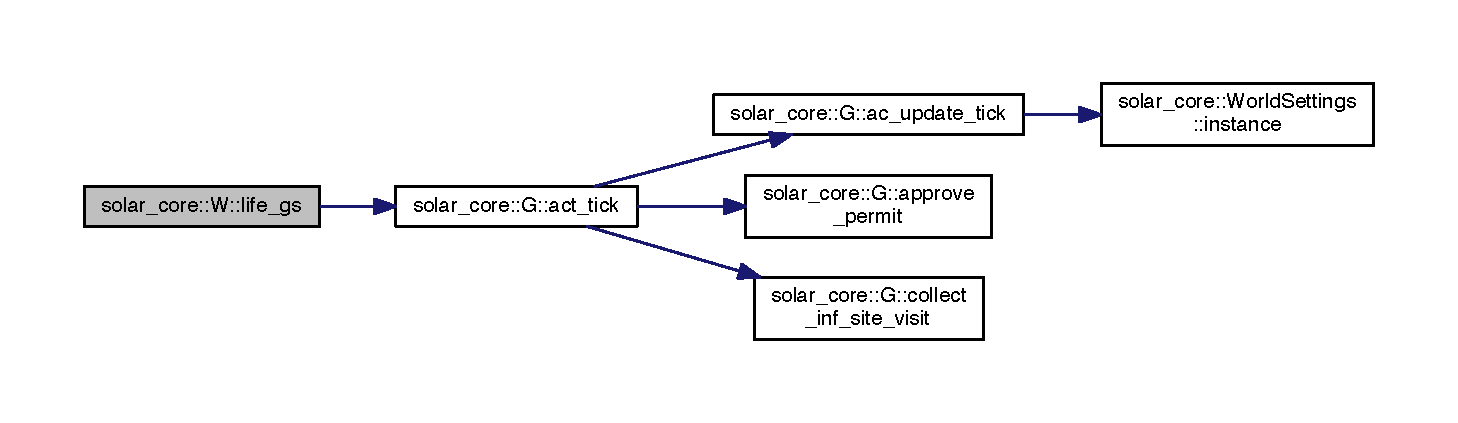
\includegraphics[width=350pt]{classsolar__core_1_1_w_ad08af315706bb42ab5dd68f41a90c978_cgraph}
\end{center}
\end{figure}

=======
Definition at line 93 of file W.\+cpp.
>>>>>>> 9fadf023062505cb443534457ab9d4d3cc1b7bfc

\hypertarget{classsolar__core_1_1_w_a08283dbea7c7f3fe8b7f094a96f73a78}{}\index{solar\+\_\+core\+::\+W@{solar\+\_\+core\+::\+W}!life\+\_\+hhs@{life\+\_\+hhs}}
\index{life\+\_\+hhs@{life\+\_\+hhs}!solar\+\_\+core\+::\+W@{solar\+\_\+core\+::\+W}}
\subsubsection[{life\+\_\+hhs}]{\setlength{\rightskip}{0pt plus 5cm}void W\+::life\+\_\+hhs (
\begin{DoxyParamCaption}
{}
\end{DoxyParamCaption}
)}\label{classsolar__core_1_1_w_a08283dbea7c7f3fe8b7f094a96f73a78}
life of households \begin{DoxyRefDesc}{Dev\+Stage3}
\item[\hyperlink{_dev_stage3__DevStage3000005}{Dev\+Stage3}]might consider moving this call to tasks, to speed up cycle. Might not be worth it as have to include the time to set up and tear down the task itself and the calls might be relatively quick. Need to profile this place. \end{DoxyRefDesc}


<<<<<<< HEAD
Definition at line 452 of file W.\+cpp.

\hypertarget{classsolar__core_1_1_w_a03a16fe70a11b947735709cf0a0b277e}{}\index{solar\+\_\+core\+::\+W@{solar\+\_\+core\+::\+W}!life\+\_\+markets@{life\+\_\+markets}}
\index{life\+\_\+markets@{life\+\_\+markets}!solar\+\_\+core\+::\+W@{solar\+\_\+core\+::\+W}}
\subsubsection[{life\+\_\+markets}]{\setlength{\rightskip}{0pt plus 5cm}void W\+::life\+\_\+markets (
\begin{DoxyParamCaption}
{}
\end{DoxyParamCaption}
)}\label{classsolar__core_1_1_w_a03a16fe70a11b947735709cf0a0b277e}
life of marketing 

Definition at line 587 of file W.\+cpp.



Here is the call graph for this function\+:
\nopagebreak
\begin{figure}[H]
\begin{center}
\leavevmode
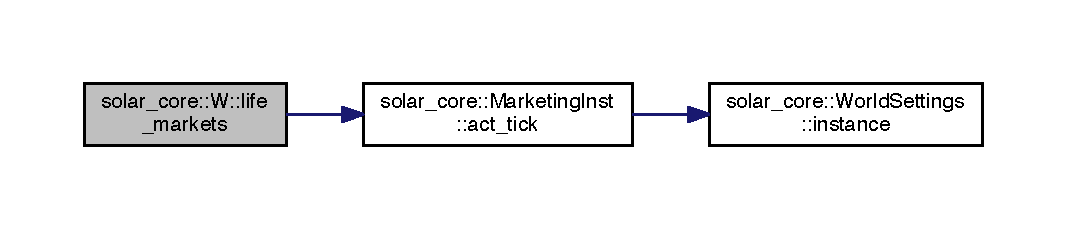
\includegraphics[width=350pt]{classsolar__core_1_1_w_a03a16fe70a11b947735709cf0a0b277e_cgraph}
\end{center}
\end{figure}


\hypertarget{classsolar__core_1_1_w_a77b206056c9440059f7b78e1424b0921}{}\index{solar\+\_\+core\+::\+W@{solar\+\_\+core\+::\+W}!life\+\_\+seis@{life\+\_\+seis}}
\index{life\+\_\+seis@{life\+\_\+seis}!solar\+\_\+core\+::\+W@{solar\+\_\+core\+::\+W}}
\subsubsection[{life\+\_\+seis}]{\setlength{\rightskip}{0pt plus 5cm}void W\+::life\+\_\+seis (
\begin{DoxyParamCaption}
{}
\end{DoxyParamCaption}
)}\label{classsolar__core_1_1_w_a77b206056c9440059f7b78e1424b0921}
life of seis 

Definition at line 499 of file W.\+cpp.

\hypertarget{classsolar__core_1_1_w_a655c14c2a3d10952ab1217eedd21443f}{}\index{solar\+\_\+core\+::\+W@{solar\+\_\+core\+::\+W}!life\+\_\+sems@{life\+\_\+sems}}
\index{life\+\_\+sems@{life\+\_\+sems}!solar\+\_\+core\+::\+W@{solar\+\_\+core\+::\+W}}
\subsubsection[{life\+\_\+sems}]{\setlength{\rightskip}{0pt plus 5cm}void W\+::life\+\_\+sems (
\begin{DoxyParamCaption}
{}
\end{DoxyParamCaption}
)}\label{classsolar__core_1_1_w_a655c14c2a3d10952ab1217eedd21443f}
life of sems 

Definition at line 528 of file W.\+cpp.



\subsection{Friends And Related Function Documentation}
\hypertarget{classsolar__core_1_1_w_ac01e54f17f927af30196b551d235d7ba}{}\index{solar\+\_\+core\+::\+W@{solar\+\_\+core\+::\+W}!Marketing\+Inst@{Marketing\+Inst}}
\index{Marketing\+Inst@{Marketing\+Inst}!solar\+\_\+core\+::\+W@{solar\+\_\+core\+::\+W}}
\subsubsection[{Marketing\+Inst}]{\setlength{\rightskip}{0pt plus 5cm}friend class {\bf Marketing\+Inst}\hspace{0.3cm}{\ttfamily [friend]}}\label{classsolar__core_1_1_w_ac01e54f17f927af30196b551d235d7ba}


Definition at line 44 of file W.\+h.

\hypertarget{classsolar__core_1_1_w_a8f3690c82c493af3a66f999410fe891d}{}\index{solar\+\_\+core\+::\+W@{solar\+\_\+core\+::\+W}!solar\+\_\+ui\+::\+U\+I@{solar\+\_\+ui\+::\+U\+I}}
\index{solar\+\_\+ui\+::\+U\+I@{solar\+\_\+ui\+::\+U\+I}!solar\+\_\+core\+::\+W@{solar\+\_\+core\+::\+W}}
\subsubsection[{solar\+\_\+ui\+::\+U\+I}]{\setlength{\rightskip}{0pt plus 5cm}friend class {\bf solar\+\_\+ui\+::\+U\+I}\hspace{0.3cm}{\ttfamily [friend]}}\label{classsolar__core_1_1_w_a8f3690c82c493af3a66f999410fe891d}


Definition at line 45 of file W.\+h.
=======
Definition at line 144 of file W.\+cpp.

\hypertarget{classsolar__core_1_1_w_a77b206056c9440059f7b78e1424b0921}{}\index{solar\+\_\+core\+::\+W@{solar\+\_\+core\+::\+W}!life\+\_\+seis@{life\+\_\+seis}}
\index{life\+\_\+seis@{life\+\_\+seis}!solar\+\_\+core\+::\+W@{solar\+\_\+core\+::\+W}}
\subsubsection[{life\+\_\+seis}]{\setlength{\rightskip}{0pt plus 5cm}void W\+::life\+\_\+seis (
\begin{DoxyParamCaption}
{}
\end{DoxyParamCaption}
)}\label{classsolar__core_1_1_w_a77b206056c9440059f7b78e1424b0921}
life of seis 

Definition at line 165 of file W.\+cpp.



\subsection{Member Data Documentation}
\hypertarget{classsolar__core_1_1_w_aa6cba0dba8a566978e51fb4204aac4b9}{}\index{solar\+\_\+core\+::\+W@{solar\+\_\+core\+::\+W}!all\+\_\+update@{all\+\_\+update}}
\index{all\+\_\+update@{all\+\_\+update}!solar\+\_\+core\+::\+W@{solar\+\_\+core\+::\+W}}
\subsubsection[{all\+\_\+update}]{\setlength{\rightskip}{0pt plus 5cm}std\+::condition\+\_\+variable solar\+\_\+core\+::\+W\+::all\+\_\+update}\label{classsolar__core_1_1_w_aa6cba0dba8a566978e51fb4204aac4b9}
waits until all have updated 
>>>>>>> 9fadf023062505cb443534457ab9d4d3cc1b7bfc

Definition at line 90 of file W.\+h.

\hypertarget{classsolar__core_1_1_w_acf6e7dd195573ba04b406cde2e5b80fb}{}\index{solar\+\_\+core\+::\+W@{solar\+\_\+core\+::\+W}!base\+\_\+path@{base\+\_\+path}}
\index{base\+\_\+path@{base\+\_\+path}!solar\+\_\+core\+::\+W@{solar\+\_\+core\+::\+W}}
\subsubsection[{base\+\_\+path}]{\setlength{\rightskip}{0pt plus 5cm}std\+::string solar\+\_\+core\+::\+W\+::base\+\_\+path}\label{classsolar__core_1_1_w_acf6e7dd195573ba04b406cde2e5b80fb}


Definition at line 47 of file W.\+h.

\hypertarget{classsolar__core_1_1_w_aec1b9014ad296dc9b8b132ba9b67c08a}{}\index{solar\+\_\+core\+::\+W@{solar\+\_\+core\+::\+W}!begin\+\_\+time@{begin\+\_\+time}}
\index{begin\+\_\+time@{begin\+\_\+time}!solar\+\_\+core\+::\+W@{solar\+\_\+core\+::\+W}}
\subsubsection[{begin\+\_\+time}]{\setlength{\rightskip}{0pt plus 5cm}{\bf Time\+Unit} solar\+\_\+core\+::\+W\+::begin\+\_\+time = 0}\label{classsolar__core_1_1_w_aec1b9014ad296dc9b8b132ba9b67c08a}


Definition at line 88 of file W.\+h.

\hypertarget{classsolar__core_1_1_w_aae63ce0d440f2c8d475d6eeafac58238}{}\index{solar\+\_\+core\+::\+W@{solar\+\_\+core\+::\+W}!F\+L\+A\+G\+\_\+\+G\+\_\+\+T\+I\+C\+K@{F\+L\+A\+G\+\_\+\+G\+\_\+\+T\+I\+C\+K}}
\index{F\+L\+A\+G\+\_\+\+G\+\_\+\+T\+I\+C\+K@{F\+L\+A\+G\+\_\+\+G\+\_\+\+T\+I\+C\+K}!solar\+\_\+core\+::\+W@{solar\+\_\+core\+::\+W}}
\subsubsection[{F\+L\+A\+G\+\_\+\+G\+\_\+\+T\+I\+C\+K}]{\setlength{\rightskip}{0pt plus 5cm}std\+::atomic$<$bool$>$ solar\+\_\+core\+::\+W\+::\+F\+L\+A\+G\+\_\+\+G\+\_\+\+T\+I\+C\+K}\label{classsolar__core_1_1_w_aae63ce0d440f2c8d475d6eeafac58238}


Definition at line 97 of file W.\+h.

\hypertarget{classsolar__core_1_1_w_a4cd32940e21bfc20919cc2d4447d66d3}{}\index{solar\+\_\+core\+::\+W@{solar\+\_\+core\+::\+W}!F\+L\+A\+G\+\_\+\+H\+\_\+\+T\+I\+C\+K@{F\+L\+A\+G\+\_\+\+H\+\_\+\+T\+I\+C\+K}}
\index{F\+L\+A\+G\+\_\+\+H\+\_\+\+T\+I\+C\+K@{F\+L\+A\+G\+\_\+\+H\+\_\+\+T\+I\+C\+K}!solar\+\_\+core\+::\+W@{solar\+\_\+core\+::\+W}}
\subsubsection[{F\+L\+A\+G\+\_\+\+H\+\_\+\+T\+I\+C\+K}]{\setlength{\rightskip}{0pt plus 5cm}std\+::atomic$<$bool$>$ solar\+\_\+core\+::\+W\+::\+F\+L\+A\+G\+\_\+\+H\+\_\+\+T\+I\+C\+K}\label{classsolar__core_1_1_w_a4cd32940e21bfc20919cc2d4447d66d3}


Definition at line 96 of file W.\+h.

\hypertarget{classsolar__core_1_1_w_a8456f88d45f2e8bf67eccd7f0c8d08fa}{}\index{solar\+\_\+core\+::\+W@{solar\+\_\+core\+::\+W}!F\+L\+A\+G\+\_\+\+I\+S\+\_\+\+S\+T\+A\+R\+T\+E\+D@{F\+L\+A\+G\+\_\+\+I\+S\+\_\+\+S\+T\+A\+R\+T\+E\+D}}
\index{F\+L\+A\+G\+\_\+\+I\+S\+\_\+\+S\+T\+A\+R\+T\+E\+D@{F\+L\+A\+G\+\_\+\+I\+S\+\_\+\+S\+T\+A\+R\+T\+E\+D}!solar\+\_\+core\+::\+W@{solar\+\_\+core\+::\+W}}
\subsubsection[{F\+L\+A\+G\+\_\+\+I\+S\+\_\+\+S\+T\+A\+R\+T\+E\+D}]{\setlength{\rightskip}{0pt plus 5cm}std\+::atomic$<$bool$>$ solar\+\_\+core\+::\+W\+::\+F\+L\+A\+G\+\_\+\+I\+S\+\_\+\+S\+T\+A\+R\+T\+E\+D}\label{classsolar__core_1_1_w_a8456f88d45f2e8bf67eccd7f0c8d08fa}


Definition at line 84 of file W.\+h.

\hypertarget{classsolar__core_1_1_w_a9bb998c65a7427961de179f41e25daea}{}\index{solar\+\_\+core\+::\+W@{solar\+\_\+core\+::\+W}!F\+L\+A\+G\+\_\+\+I\+S\+\_\+\+S\+T\+O\+P\+P\+E\+D@{F\+L\+A\+G\+\_\+\+I\+S\+\_\+\+S\+T\+O\+P\+P\+E\+D}}
\index{F\+L\+A\+G\+\_\+\+I\+S\+\_\+\+S\+T\+O\+P\+P\+E\+D@{F\+L\+A\+G\+\_\+\+I\+S\+\_\+\+S\+T\+O\+P\+P\+E\+D}!solar\+\_\+core\+::\+W@{solar\+\_\+core\+::\+W}}
\subsubsection[{F\+L\+A\+G\+\_\+\+I\+S\+\_\+\+S\+T\+O\+P\+P\+E\+D}]{\setlength{\rightskip}{0pt plus 5cm}std\+::atomic$<$bool$>$ solar\+\_\+core\+::\+W\+::\+F\+L\+A\+G\+\_\+\+I\+S\+\_\+\+S\+T\+O\+P\+P\+E\+D}\label{classsolar__core_1_1_w_a9bb998c65a7427961de179f41e25daea}
Section with general world parameters and etc. 

Definition at line 83 of file W.\+h.

\hypertarget{classsolar__core_1_1_w_a65d2047e574ed6201a8e21ec1ba1bec4}{}\index{solar\+\_\+core\+::\+W@{solar\+\_\+core\+::\+W}!F\+L\+A\+G\+\_\+\+S\+E\+I\+\_\+\+T\+I\+C\+K@{F\+L\+A\+G\+\_\+\+S\+E\+I\+\_\+\+T\+I\+C\+K}}
\index{F\+L\+A\+G\+\_\+\+S\+E\+I\+\_\+\+T\+I\+C\+K@{F\+L\+A\+G\+\_\+\+S\+E\+I\+\_\+\+T\+I\+C\+K}!solar\+\_\+core\+::\+W@{solar\+\_\+core\+::\+W}}
\subsubsection[{F\+L\+A\+G\+\_\+\+S\+E\+I\+\_\+\+T\+I\+C\+K}]{\setlength{\rightskip}{0pt plus 5cm}std\+::atomic$<$bool$>$ solar\+\_\+core\+::\+W\+::\+F\+L\+A\+G\+\_\+\+S\+E\+I\+\_\+\+T\+I\+C\+K}\label{classsolar__core_1_1_w_a65d2047e574ed6201a8e21ec1ba1bec4}


Definition at line 95 of file W.\+h.

\hypertarget{classsolar__core_1_1_w_ae383b7a595cb28d52aa747fc7e5bb619}{}\index{solar\+\_\+core\+::\+W@{solar\+\_\+core\+::\+W}!F\+L\+A\+G\+\_\+\+S\+E\+M\+\_\+\+T\+I\+C\+K@{F\+L\+A\+G\+\_\+\+S\+E\+M\+\_\+\+T\+I\+C\+K}}
\index{F\+L\+A\+G\+\_\+\+S\+E\+M\+\_\+\+T\+I\+C\+K@{F\+L\+A\+G\+\_\+\+S\+E\+M\+\_\+\+T\+I\+C\+K}!solar\+\_\+core\+::\+W@{solar\+\_\+core\+::\+W}}
\subsubsection[{F\+L\+A\+G\+\_\+\+S\+E\+M\+\_\+\+T\+I\+C\+K}]{\setlength{\rightskip}{0pt plus 5cm}std\+::atomic$<$bool$>$ solar\+\_\+core\+::\+W\+::\+F\+L\+A\+G\+\_\+\+S\+E\+M\+\_\+\+T\+I\+C\+K}\label{classsolar__core_1_1_w_ae383b7a595cb28d52aa747fc7e5bb619}


Definition at line 98 of file W.\+h.

\hypertarget{classsolar__core_1_1_w_a9e50ef0da579cdfc3da22c16a492bc44}{}\index{solar\+\_\+core\+::\+W@{solar\+\_\+core\+::\+W}!g@{g}}
\index{g@{g}!solar\+\_\+core\+::\+W@{solar\+\_\+core\+::\+W}}
\subsubsection[{g}]{\setlength{\rightskip}{0pt plus 5cm}{\bf G}$\ast$ solar\+\_\+core\+::\+W\+::g}\label{classsolar__core_1_1_w_a9e50ef0da579cdfc3da22c16a492bc44}
Geography 

Definition at line 124 of file W.\+h.

<<<<<<< HEAD
\subsection{Member Data Documentation}
\hypertarget{classsolar__core_1_1_w_aa6cba0dba8a566978e51fb4204aac4b9}{}\index{solar\+\_\+core\+::\+W@{solar\+\_\+core\+::\+W}!all\+\_\+update@{all\+\_\+update}}
\index{all\+\_\+update@{all\+\_\+update}!solar\+\_\+core\+::\+W@{solar\+\_\+core\+::\+W}}
\subsubsection[{all\+\_\+update}]{\setlength{\rightskip}{0pt plus 5cm}std\+::condition\+\_\+variable solar\+\_\+core\+::\+W\+::all\+\_\+update}\label{classsolar__core_1_1_w_aa6cba0dba8a566978e51fb4204aac4b9}
waits until all have updated 

Definition at line 111 of file W.\+h.

\hypertarget{classsolar__core_1_1_w_acf6e7dd195573ba04b406cde2e5b80fb}{}\index{solar\+\_\+core\+::\+W@{solar\+\_\+core\+::\+W}!base\+\_\+path@{base\+\_\+path}}
\index{base\+\_\+path@{base\+\_\+path}!solar\+\_\+core\+::\+W@{solar\+\_\+core\+::\+W}}
\subsubsection[{base\+\_\+path}]{\setlength{\rightskip}{0pt plus 5cm}std\+::string solar\+\_\+core\+::\+W\+::base\+\_\+path}\label{classsolar__core_1_1_w_acf6e7dd195573ba04b406cde2e5b80fb}


Definition at line 61 of file W.\+h.

\hypertarget{classsolar__core_1_1_w_aec1b9014ad296dc9b8b132ba9b67c08a}{}\index{solar\+\_\+core\+::\+W@{solar\+\_\+core\+::\+W}!begin\+\_\+time@{begin\+\_\+time}}
\index{begin\+\_\+time@{begin\+\_\+time}!solar\+\_\+core\+::\+W@{solar\+\_\+core\+::\+W}}
\subsubsection[{begin\+\_\+time}]{\setlength{\rightskip}{0pt plus 5cm}{\bf Time\+Unit} solar\+\_\+core\+::\+W\+::begin\+\_\+time = 0}\label{classsolar__core_1_1_w_aec1b9014ad296dc9b8b132ba9b67c08a}


Definition at line 109 of file W.\+h.

\hypertarget{classsolar__core_1_1_w_aae63ce0d440f2c8d475d6eeafac58238}{}\index{solar\+\_\+core\+::\+W@{solar\+\_\+core\+::\+W}!F\+L\+A\+G\+\_\+\+G\+\_\+\+T\+I\+C\+K@{F\+L\+A\+G\+\_\+\+G\+\_\+\+T\+I\+C\+K}}
\index{F\+L\+A\+G\+\_\+\+G\+\_\+\+T\+I\+C\+K@{F\+L\+A\+G\+\_\+\+G\+\_\+\+T\+I\+C\+K}!solar\+\_\+core\+::\+W@{solar\+\_\+core\+::\+W}}
\subsubsection[{F\+L\+A\+G\+\_\+\+G\+\_\+\+T\+I\+C\+K}]{\setlength{\rightskip}{0pt plus 5cm}std\+::atomic$<$bool$>$ solar\+\_\+core\+::\+W\+::\+F\+L\+A\+G\+\_\+\+G\+\_\+\+T\+I\+C\+K}\label{classsolar__core_1_1_w_aae63ce0d440f2c8d475d6eeafac58238}


Definition at line 118 of file W.\+h.

\hypertarget{classsolar__core_1_1_w_a4cd32940e21bfc20919cc2d4447d66d3}{}\index{solar\+\_\+core\+::\+W@{solar\+\_\+core\+::\+W}!F\+L\+A\+G\+\_\+\+H\+\_\+\+T\+I\+C\+K@{F\+L\+A\+G\+\_\+\+H\+\_\+\+T\+I\+C\+K}}
\index{F\+L\+A\+G\+\_\+\+H\+\_\+\+T\+I\+C\+K@{F\+L\+A\+G\+\_\+\+H\+\_\+\+T\+I\+C\+K}!solar\+\_\+core\+::\+W@{solar\+\_\+core\+::\+W}}
\subsubsection[{F\+L\+A\+G\+\_\+\+H\+\_\+\+T\+I\+C\+K}]{\setlength{\rightskip}{0pt plus 5cm}std\+::atomic$<$bool$>$ solar\+\_\+core\+::\+W\+::\+F\+L\+A\+G\+\_\+\+H\+\_\+\+T\+I\+C\+K}\label{classsolar__core_1_1_w_a4cd32940e21bfc20919cc2d4447d66d3}


Definition at line 117 of file W.\+h.

\hypertarget{classsolar__core_1_1_w_a1c0ebdba727a7a5cbf322072ab5c9184}{}\index{solar\+\_\+core\+::\+W@{solar\+\_\+core\+::\+W}!F\+L\+A\+G\+\_\+\+I\+S\+\_\+\+P\+A\+U\+S\+E\+D@{F\+L\+A\+G\+\_\+\+I\+S\+\_\+\+P\+A\+U\+S\+E\+D}}
\index{F\+L\+A\+G\+\_\+\+I\+S\+\_\+\+P\+A\+U\+S\+E\+D@{F\+L\+A\+G\+\_\+\+I\+S\+\_\+\+P\+A\+U\+S\+E\+D}!solar\+\_\+core\+::\+W@{solar\+\_\+core\+::\+W}}
\subsubsection[{F\+L\+A\+G\+\_\+\+I\+S\+\_\+\+P\+A\+U\+S\+E\+D}]{\setlength{\rightskip}{0pt plus 5cm}std\+::atomic$<$bool$>$ solar\+\_\+core\+::\+W\+::\+F\+L\+A\+G\+\_\+\+I\+S\+\_\+\+P\+A\+U\+S\+E\+D}\label{classsolar__core_1_1_w_a1c0ebdba727a7a5cbf322072ab5c9184}


Definition at line 106 of file W.\+h.

\hypertarget{classsolar__core_1_1_w_a8456f88d45f2e8bf67eccd7f0c8d08fa}{}\index{solar\+\_\+core\+::\+W@{solar\+\_\+core\+::\+W}!F\+L\+A\+G\+\_\+\+I\+S\+\_\+\+S\+T\+A\+R\+T\+E\+D@{F\+L\+A\+G\+\_\+\+I\+S\+\_\+\+S\+T\+A\+R\+T\+E\+D}}
\index{F\+L\+A\+G\+\_\+\+I\+S\+\_\+\+S\+T\+A\+R\+T\+E\+D@{F\+L\+A\+G\+\_\+\+I\+S\+\_\+\+S\+T\+A\+R\+T\+E\+D}!solar\+\_\+core\+::\+W@{solar\+\_\+core\+::\+W}}
\subsubsection[{F\+L\+A\+G\+\_\+\+I\+S\+\_\+\+S\+T\+A\+R\+T\+E\+D}]{\setlength{\rightskip}{0pt plus 5cm}std\+::atomic$<$bool$>$ solar\+\_\+core\+::\+W\+::\+F\+L\+A\+G\+\_\+\+I\+S\+\_\+\+S\+T\+A\+R\+T\+E\+D}\label{classsolar__core_1_1_w_a8456f88d45f2e8bf67eccd7f0c8d08fa}


Definition at line 105 of file W.\+h.

\hypertarget{classsolar__core_1_1_w_a9bb998c65a7427961de179f41e25daea}{}\index{solar\+\_\+core\+::\+W@{solar\+\_\+core\+::\+W}!F\+L\+A\+G\+\_\+\+I\+S\+\_\+\+S\+T\+O\+P\+P\+E\+D@{F\+L\+A\+G\+\_\+\+I\+S\+\_\+\+S\+T\+O\+P\+P\+E\+D}}
\index{F\+L\+A\+G\+\_\+\+I\+S\+\_\+\+S\+T\+O\+P\+P\+E\+D@{F\+L\+A\+G\+\_\+\+I\+S\+\_\+\+S\+T\+O\+P\+P\+E\+D}!solar\+\_\+core\+::\+W@{solar\+\_\+core\+::\+W}}
\subsubsection[{F\+L\+A\+G\+\_\+\+I\+S\+\_\+\+S\+T\+O\+P\+P\+E\+D}]{\setlength{\rightskip}{0pt plus 5cm}std\+::atomic$<$bool$>$ solar\+\_\+core\+::\+W\+::\+F\+L\+A\+G\+\_\+\+I\+S\+\_\+\+S\+T\+O\+P\+P\+E\+D}\label{classsolar__core_1_1_w_a9bb998c65a7427961de179f41e25daea}
Section with general world parameters and etc. 

Definition at line 104 of file W.\+h.

\hypertarget{classsolar__core_1_1_w_a7aa8b882244539e098e45207045d7d88}{}\index{solar\+\_\+core\+::\+W@{solar\+\_\+core\+::\+W}!F\+L\+A\+G\+\_\+\+M\+A\+R\+K\+E\+T\+\_\+\+T\+I\+C\+K@{F\+L\+A\+G\+\_\+\+M\+A\+R\+K\+E\+T\+\_\+\+T\+I\+C\+K}}
\index{F\+L\+A\+G\+\_\+\+M\+A\+R\+K\+E\+T\+\_\+\+T\+I\+C\+K@{F\+L\+A\+G\+\_\+\+M\+A\+R\+K\+E\+T\+\_\+\+T\+I\+C\+K}!solar\+\_\+core\+::\+W@{solar\+\_\+core\+::\+W}}
\subsubsection[{F\+L\+A\+G\+\_\+\+M\+A\+R\+K\+E\+T\+\_\+\+T\+I\+C\+K}]{\setlength{\rightskip}{0pt plus 5cm}std\+::atomic$<$bool$>$ solar\+\_\+core\+::\+W\+::\+F\+L\+A\+G\+\_\+\+M\+A\+R\+K\+E\+T\+\_\+\+T\+I\+C\+K}\label{classsolar__core_1_1_w_a7aa8b882244539e098e45207045d7d88}


Definition at line 119 of file W.\+h.

\hypertarget{classsolar__core_1_1_w_a65d2047e574ed6201a8e21ec1ba1bec4}{}\index{solar\+\_\+core\+::\+W@{solar\+\_\+core\+::\+W}!F\+L\+A\+G\+\_\+\+S\+E\+I\+\_\+\+T\+I\+C\+K@{F\+L\+A\+G\+\_\+\+S\+E\+I\+\_\+\+T\+I\+C\+K}}
\index{F\+L\+A\+G\+\_\+\+S\+E\+I\+\_\+\+T\+I\+C\+K@{F\+L\+A\+G\+\_\+\+S\+E\+I\+\_\+\+T\+I\+C\+K}!solar\+\_\+core\+::\+W@{solar\+\_\+core\+::\+W}}
\subsubsection[{F\+L\+A\+G\+\_\+\+S\+E\+I\+\_\+\+T\+I\+C\+K}]{\setlength{\rightskip}{0pt plus 5cm}std\+::atomic$<$bool$>$ solar\+\_\+core\+::\+W\+::\+F\+L\+A\+G\+\_\+\+S\+E\+I\+\_\+\+T\+I\+C\+K}\label{classsolar__core_1_1_w_a65d2047e574ed6201a8e21ec1ba1bec4}


Definition at line 116 of file W.\+h.

\hypertarget{classsolar__core_1_1_w_ae383b7a595cb28d52aa747fc7e5bb619}{}\index{solar\+\_\+core\+::\+W@{solar\+\_\+core\+::\+W}!F\+L\+A\+G\+\_\+\+S\+E\+M\+\_\+\+T\+I\+C\+K@{F\+L\+A\+G\+\_\+\+S\+E\+M\+\_\+\+T\+I\+C\+K}}
\index{F\+L\+A\+G\+\_\+\+S\+E\+M\+\_\+\+T\+I\+C\+K@{F\+L\+A\+G\+\_\+\+S\+E\+M\+\_\+\+T\+I\+C\+K}!solar\+\_\+core\+::\+W@{solar\+\_\+core\+::\+W}}
\subsubsection[{F\+L\+A\+G\+\_\+\+S\+E\+M\+\_\+\+T\+I\+C\+K}]{\setlength{\rightskip}{0pt plus 5cm}std\+::atomic$<$bool$>$ solar\+\_\+core\+::\+W\+::\+F\+L\+A\+G\+\_\+\+S\+E\+M\+\_\+\+T\+I\+C\+K}\label{classsolar__core_1_1_w_ae383b7a595cb28d52aa747fc7e5bb619}


Definition at line 120 of file W.\+h.

\hypertarget{classsolar__core_1_1_w_a9e50ef0da579cdfc3da22c16a492bc44}{}\index{solar\+\_\+core\+::\+W@{solar\+\_\+core\+::\+W}!g@{g}}
\index{g@{g}!solar\+\_\+core\+::\+W@{solar\+\_\+core\+::\+W}}
\subsubsection[{g}]{\setlength{\rightskip}{0pt plus 5cm}{\bf G}$\ast$ solar\+\_\+core\+::\+W\+::g}\label{classsolar__core_1_1_w_a9e50ef0da579cdfc3da22c16a492bc44}
Institutionsgovernment 

Definition at line 167 of file W.\+h.

=======
>>>>>>> 9fadf023062505cb443534457ab9d4d3cc1b7bfc
\hypertarget{classsolar__core_1_1_w_a81b5469757f203c9619ff69323ac0f77}{}\index{solar\+\_\+core\+::\+W@{solar\+\_\+core\+::\+W}!get\+\_\+inf\+\_\+marketing\+\_\+sei\+\_\+agents@{get\+\_\+inf\+\_\+marketing\+\_\+sei\+\_\+agents}}
\index{get\+\_\+inf\+\_\+marketing\+\_\+sei\+\_\+agents@{get\+\_\+inf\+\_\+marketing\+\_\+sei\+\_\+agents}!solar\+\_\+core\+::\+W@{solar\+\_\+core\+::\+W}}
\subsubsection[{get\+\_\+inf\+\_\+marketing\+\_\+sei\+\_\+agents}]{\setlength{\rightskip}{0pt plus 5cm}std\+::deque$<${\bf I\+Agent}$\ast$$>$ solar\+\_\+core\+::\+W\+::get\+\_\+inf\+\_\+marketing\+\_\+sei\+\_\+agents\hspace{0.3cm}{\ttfamily [protected]}}\label{classsolar__core_1_1_w_a81b5469757f203c9619ff69323ac0f77}
Agents that requested information, inform \hyperlink{classsolar__core_1_1_s_e_i}{S\+E\+I} that there is request for information for this agent 

<<<<<<< HEAD
Definition at line 176 of file W.\+h.
=======
Definition at line 130 of file W.\+h.
>>>>>>> 9fadf023062505cb443534457ab9d4d3cc1b7bfc

\hypertarget{classsolar__core_1_1_w_a17c012ff8b17890ed33923cec6d87be3}{}\index{solar\+\_\+core\+::\+W@{solar\+\_\+core\+::\+W}!hhs@{hhs}}
\index{hhs@{hhs}!solar\+\_\+core\+::\+W@{solar\+\_\+core\+::\+W}}
\subsubsection[{hhs}]{\setlength{\rightskip}{0pt plus 5cm}std\+::vector$<${\bf Household}$\ast$$>$ solar\+\_\+core\+::\+W\+::hhs\hspace{0.3cm}{\ttfamily [protected]}}\label{classsolar__core_1_1_w_a17c012ff8b17890ed33923cec6d87be3}
all H agents 

<<<<<<< HEAD
Definition at line 180 of file W.\+h.

\hypertarget{classsolar__core_1_1_w_a1d35d6501eef6d673bd2b28e2c1724c4}{}\index{solar\+\_\+core\+::\+W@{solar\+\_\+core\+::\+W}!interconnected\+\_\+projects@{interconnected\+\_\+projects}}
\index{interconnected\+\_\+projects@{interconnected\+\_\+projects}!solar\+\_\+core\+::\+W@{solar\+\_\+core\+::\+W}}
\subsubsection[{interconnected\+\_\+projects}]{\setlength{\rightskip}{0pt plus 5cm}std\+::vector$<$std\+::shared\+\_\+ptr$<${\bf P\+V\+Project}$>$ $>$ solar\+\_\+core\+::\+W\+::interconnected\+\_\+projects\hspace{0.3cm}{\ttfamily [protected]}}\label{classsolar__core_1_1_w_a1d35d6501eef6d673bd2b28e2c1724c4}
\begin{DoxyRefDesc}{Dev\+Stage2}
\item[\hyperlink{_dev_stage2__DevStage2000030}{Dev\+Stage2}]think here, might change to weak\+\_\+ptr, but will pay the cost of checking each time if it is still alive \end{DoxyRefDesc}


Definition at line 188 of file W.\+h.
=======
Definition at line 134 of file W.\+h.
>>>>>>> 9fadf023062505cb443534457ab9d4d3cc1b7bfc

\hypertarget{classsolar__core_1_1_w_a56ba20ee51f5db7288e55bb65f12511b}{}\index{solar\+\_\+core\+::\+W@{solar\+\_\+core\+::\+W}!lock\+\_\+tick@{lock\+\_\+tick}}
\index{lock\+\_\+tick@{lock\+\_\+tick}!solar\+\_\+core\+::\+W@{solar\+\_\+core\+::\+W}}
\subsubsection[{lock\+\_\+tick}]{\setlength{\rightskip}{0pt plus 5cm}std\+::mutex solar\+\_\+core\+::\+W\+::lock\+\_\+tick}\label{classsolar__core_1_1_w_a56ba20ee51f5db7288e55bb65f12511b}
lock for tick 

<<<<<<< HEAD
Definition at line 110 of file W.\+h.

\hypertarget{classsolar__core_1_1_w_a93f277fb3a9d9e7b1e911c6a494c8ec8}{}\index{solar\+\_\+core\+::\+W@{solar\+\_\+core\+::\+W}!marketing@{marketing}}
\index{marketing@{marketing}!solar\+\_\+core\+::\+W@{solar\+\_\+core\+::\+W}}
\subsubsection[{marketing}]{\setlength{\rightskip}{0pt plus 5cm}{\bf Marketing\+Inst}$\ast$ solar\+\_\+core\+::\+W\+::marketing}\label{classsolar__core_1_1_w_a93f277fb3a9d9e7b1e911c6a494c8ec8}


Definition at line 168 of file W.\+h.
=======
Definition at line 89 of file W.\+h.
>>>>>>> 9fadf023062505cb443534457ab9d4d3cc1b7bfc

\hypertarget{classsolar__core_1_1_w_afee32d515534826a60ddf12936f85a3d}{}\index{solar\+\_\+core\+::\+W@{solar\+\_\+core\+::\+W}!notified\+\_\+counter@{notified\+\_\+counter}}
\index{notified\+\_\+counter@{notified\+\_\+counter}!solar\+\_\+core\+::\+W@{solar\+\_\+core\+::\+W}}
\subsubsection[{notified\+\_\+counter}]{\setlength{\rightskip}{0pt plus 5cm}std\+::atomic$<$long$>$ solar\+\_\+core\+::\+W\+::notified\+\_\+counter}\label{classsolar__core_1_1_w_afee32d515534826a60ddf12936f85a3d}


<<<<<<< HEAD
Definition at line 114 of file W.\+h.
=======
Definition at line 93 of file W.\+h.
>>>>>>> 9fadf023062505cb443534457ab9d4d3cc1b7bfc

\hypertarget{classsolar__core_1_1_w_a0d06bc7242f8b3958986118eb217583f}{}\index{solar\+\_\+core\+::\+W@{solar\+\_\+core\+::\+W}!params@{params}}
\index{params@{params}!solar\+\_\+core\+::\+W@{solar\+\_\+core\+::\+W}}
\subsubsection[{params}]{\setlength{\rightskip}{0pt plus 5cm}std\+::map$<$std\+::string, std\+::string$>$ solar\+\_\+core\+::\+W\+::params\hspace{0.3cm}{\ttfamily [protected]}}\label{classsolar__core_1_1_w_a0d06bc7242f8b3958986118eb217583f}


<<<<<<< HEAD
Definition at line 185 of file W.\+h.

\hypertarget{classsolar__core_1_1_w_aa60afb55012cd72e304ac2c133e5a245}{}\index{solar\+\_\+core\+::\+W@{solar\+\_\+core\+::\+W}!rand@{rand}}
\index{rand@{rand}!solar\+\_\+core\+::\+W@{solar\+\_\+core\+::\+W}}
\subsubsection[{rand}]{\setlength{\rightskip}{0pt plus 5cm}{\bf I\+Random}$\ast$ solar\+\_\+core\+::\+W\+::rand = nullptr}\label{classsolar__core_1_1_w_aa60afb55012cd72e304ac2c133e5a245}
random number generator, same for everyone for now 

Definition at line 123 of file W.\+h.
=======
Definition at line 139 of file W.\+h.
>>>>>>> 9fadf023062505cb443534457ab9d4d3cc1b7bfc

\hypertarget{classsolar__core_1_1_w_a311baa30390494ae8e79f26e372e716d}{}\index{solar\+\_\+core\+::\+W@{solar\+\_\+core\+::\+W}!seis@{seis}}
\index{seis@{seis}!solar\+\_\+core\+::\+W@{solar\+\_\+core\+::\+W}}
\subsubsection[{seis}]{\setlength{\rightskip}{0pt plus 5cm}std\+::vector$<${\bf S\+E\+I}$\ast$$>$ solar\+\_\+core\+::\+W\+::seis\hspace{0.3cm}{\ttfamily [protected]}}\label{classsolar__core_1_1_w_a311baa30390494ae8e79f26e372e716d}
all \hyperlink{classsolar__core_1_1_s_e_i}{S\+E\+I} agents 

<<<<<<< HEAD
Definition at line 181 of file W.\+h.

\hypertarget{classsolar__core_1_1_w_ab6349cbc751747a05618dad4ebb1b726}{}\index{solar\+\_\+core\+::\+W@{solar\+\_\+core\+::\+W}!sems@{sems}}
\index{sems@{sems}!solar\+\_\+core\+::\+W@{solar\+\_\+core\+::\+W}}
\subsubsection[{sems}]{\setlength{\rightskip}{0pt plus 5cm}std\+::vector$<${\bf S\+E\+M}$\ast$$>$ solar\+\_\+core\+::\+W\+::sems\hspace{0.3cm}{\ttfamily [protected]}}\label{classsolar__core_1_1_w_ab6349cbc751747a05618dad4ebb1b726}
all \hyperlink{classsolar__core_1_1_s_e_m}{S\+E\+M} H agents that are active,\begin{DoxyRefDesc}{Dev\+Stage3}
\item[\hyperlink{_dev_stage3__DevStage3000006}{Dev\+Stage3}]think about splitting more fine grained \end{DoxyRefDesc}


Definition at line 182 of file W.\+h.
=======
Definition at line 135 of file W.\+h.

\hypertarget{classsolar__core_1_1_w_ab6349cbc751747a05618dad4ebb1b726}{}\index{solar\+\_\+core\+::\+W@{solar\+\_\+core\+::\+W}!sems@{sems}}
\index{sems@{sems}!solar\+\_\+core\+::\+W@{solar\+\_\+core\+::\+W}}
\subsubsection[{sems}]{\setlength{\rightskip}{0pt plus 5cm}std\+::vector$<$S\+E\+M$\ast$$>$ solar\+\_\+core\+::\+W\+::sems\hspace{0.3cm}{\ttfamily [protected]}}\label{classsolar__core_1_1_w_ab6349cbc751747a05618dad4ebb1b726}
all S\+E\+M H agents that are active,\begin{DoxyRefDesc}{Dev\+Stage3}
\item[\hyperlink{_dev_stage3__DevStage3000006}{Dev\+Stage3}]think about splitting more fine grained \end{DoxyRefDesc}


Definition at line 136 of file W.\+h.
>>>>>>> 9fadf023062505cb443534457ab9d4d3cc1b7bfc

\hypertarget{classsolar__core_1_1_w_ae96b30122adc9fae8fc2f209a4c89b0a}{}\index{solar\+\_\+core\+::\+W@{solar\+\_\+core\+::\+W}!time@{time}}
\index{time@{time}!solar\+\_\+core\+::\+W@{solar\+\_\+core\+::\+W}}
\subsubsection[{time}]{\setlength{\rightskip}{0pt plus 5cm}{\bf Time\+Unit} solar\+\_\+core\+::\+W\+::time}\label{classsolar__core_1_1_w_ae96b30122adc9fae8fc2f209a4c89b0a}


<<<<<<< HEAD
Definition at line 108 of file W.\+h.
=======
Definition at line 87 of file W.\+h.
>>>>>>> 9fadf023062505cb443534457ab9d4d3cc1b7bfc

\hypertarget{classsolar__core_1_1_w_a775d817c6117b462571c3fca62fe0c86}{}\index{solar\+\_\+core\+::\+W@{solar\+\_\+core\+::\+W}!updated\+\_\+counter@{updated\+\_\+counter}}
\index{updated\+\_\+counter@{updated\+\_\+counter}!solar\+\_\+core\+::\+W@{solar\+\_\+core\+::\+W}}
\subsubsection[{updated\+\_\+counter}]{\setlength{\rightskip}{0pt plus 5cm}std\+::atomic$<$long$>$ solar\+\_\+core\+::\+W\+::updated\+\_\+counter}\label{classsolar__core_1_1_w_a775d817c6117b462571c3fca62fe0c86}


<<<<<<< HEAD
Definition at line 113 of file W.\+h.

\hypertarget{classsolar__core_1_1_w_a6d6fa51d4bdc40dac8b76aa4967030b5}{}\index{solar\+\_\+core\+::\+W@{solar\+\_\+core\+::\+W}!utility@{utility}}
\index{utility@{utility}!solar\+\_\+core\+::\+W@{solar\+\_\+core\+::\+W}}
\subsubsection[{utility}]{\setlength{\rightskip}{0pt plus 5cm}{\bf Utility}$\ast$ solar\+\_\+core\+::\+W\+::utility}\label{classsolar__core_1_1_w_a6d6fa51d4bdc40dac8b76aa4967030b5}


Definition at line 169 of file W.\+h.

\hypertarget{classsolar__core_1_1_w_a8ed6f1aa7fd4ef2c3488147b38a670b7}{}\index{solar\+\_\+core\+::\+W@{solar\+\_\+core\+::\+W}!world\+\_\+map@{world\+\_\+map}}
\index{world\+\_\+map@{world\+\_\+map}!solar\+\_\+core\+::\+W@{solar\+\_\+core\+::\+W}}
\subsubsection[{world\+\_\+map}]{\setlength{\rightskip}{0pt plus 5cm}{\bf World\+Map}$\ast$ solar\+\_\+core\+::\+W\+::world\+\_\+map}\label{classsolar__core_1_1_w_a8ed6f1aa7fd4ef2c3488147b38a670b7}


Definition at line 137 of file W.\+h.
=======
Definition at line 92 of file W.\+h.

\hypertarget{classsolar__core_1_1_w_a8ed6f1aa7fd4ef2c3488147b38a670b7}{}\index{solar\+\_\+core\+::\+W@{solar\+\_\+core\+::\+W}!world\+\_\+map@{world\+\_\+map}}
\index{world\+\_\+map@{world\+\_\+map}!solar\+\_\+core\+::\+W@{solar\+\_\+core\+::\+W}}
\subsubsection[{world\+\_\+map}]{\setlength{\rightskip}{0pt plus 5cm}{\bf World\+Map}$\ast$ solar\+\_\+core\+::\+W\+::world\+\_\+map\hspace{0.3cm}{\ttfamily [protected]}}\label{classsolar__core_1_1_w_a8ed6f1aa7fd4ef2c3488147b38a670b7}


Definition at line 141 of file W.\+h.
>>>>>>> 9fadf023062505cb443534457ab9d4d3cc1b7bfc



The documentation for this class was generated from the following files\+:\begin{DoxyCompactItemize}
\item 
/\+Users/wilfeli/\+Dropbox/\+A\+B\+M/\+Solar\+Panels/\+A\+B\+M\+I\+R\+I\+S\+Lab/\+Source/\+U\+I/\hyperlink{_w_8h}{W.\+h}\item 
/\+Users/wilfeli/\+Dropbox/\+A\+B\+M/\+Solar\+Panels/\+A\+B\+M\+I\+R\+I\+S\+Lab/\+Source/\+U\+I/\hyperlink{_w_8cpp}{W.\+cpp}\end{DoxyCompactItemize}

\hypertarget{class_world_map}{}\section{World\+Map Class Reference}
\label{class_world_map}\index{World\+Map@{World\+Map}}


{\ttfamily \#include $<$Geography.\+h$>$}



Collaboration diagram for World\+Map\+:\nopagebreak
\begin{figure}[H]
\begin{center}
\leavevmode
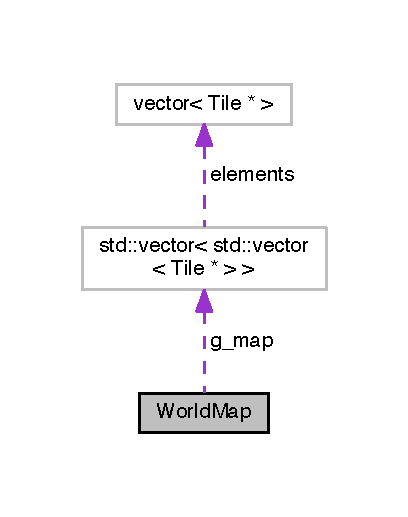
\includegraphics[width=196pt]{class_world_map__coll__graph}
\end{center}
\end{figure}
\subsection*{Public Attributes}
\begin{DoxyCompactItemize}
\item 
std\+::vector$<$ std\+::vector$<$ \hyperlink{class_tile}{Tile} $\ast$ $>$ $>$ \hyperlink{class_world_map_af3793bf3fcd5d16b5077fb07586f1dbb}{g\+\_\+map}
\end{DoxyCompactItemize}


\subsection{Detailed Description}


Definition at line 64 of file Geography.\+h.



\subsection{Member Data Documentation}
\hypertarget{class_world_map_af3793bf3fcd5d16b5077fb07586f1dbb}{}\index{World\+Map@{World\+Map}!g\+\_\+map@{g\+\_\+map}}
\index{g\+\_\+map@{g\+\_\+map}!World\+Map@{World\+Map}}
\subsubsection[{g\+\_\+map}]{\setlength{\rightskip}{0pt plus 5cm}std\+::vector$<$std\+::vector$<${\bf Tile}$\ast$$>$ $>$ World\+Map\+::g\+\_\+map}\label{class_world_map_af3793bf3fcd5d16b5077fb07586f1dbb}
grid of location tiles 

Definition at line 67 of file Geography.\+h.



The documentation for this class was generated from the following file\+:\begin{DoxyCompactItemize}
\item 
/\+Users/wilfeli/\+Dropbox/\+A\+B\+M/\+Solar\+Panels/\+A\+B\+M\+I\+R\+I\+S\+Lab/\+Source/\+Geography/\hyperlink{_geography_8h}{Geography.\+h}\end{DoxyCompactItemize}

\chapter{File Documentation}
\hypertarget{_h_8h}{}\section{/\+Users/wilfeli/\+Dropbox/\+A\+B\+M/\+Solar\+Panels/\+A\+B\+M\+I\+R\+I\+S\+Lab/\+Source/\+Agents/\+H.h File Reference}
\label{_h_8h}\index{/\+Users/wilfeli/\+Dropbox/\+A\+B\+M/\+Solar\+Panels/\+A\+B\+M\+I\+R\+I\+S\+Lab/\+Source/\+Agents/\+H.\+h@{/\+Users/wilfeli/\+Dropbox/\+A\+B\+M/\+Solar\+Panels/\+A\+B\+M\+I\+R\+I\+S\+Lab/\+Source/\+Agents/\+H.\+h}}
{\ttfamily \#include \char`\"{}Tools/\+External\+Includes.\+h\char`\"{}}\\*
{\ttfamily \#include $<$mutex$>$}\\*
{\ttfamily \#include \char`\"{}Tools/\+I\+Parameters.\+h\char`\"{}}\\*
{\ttfamily \#include \char`\"{}Geography/\+Geography.\+h\char`\"{}}\\*
{\ttfamily \#include \char`\"{}Agents/\+I\+Agent.\+h\char`\"{}}\\*
Include dependency graph for H.\+h\+:
\nopagebreak
\begin{figure}[H]
\begin{center}
\leavevmode
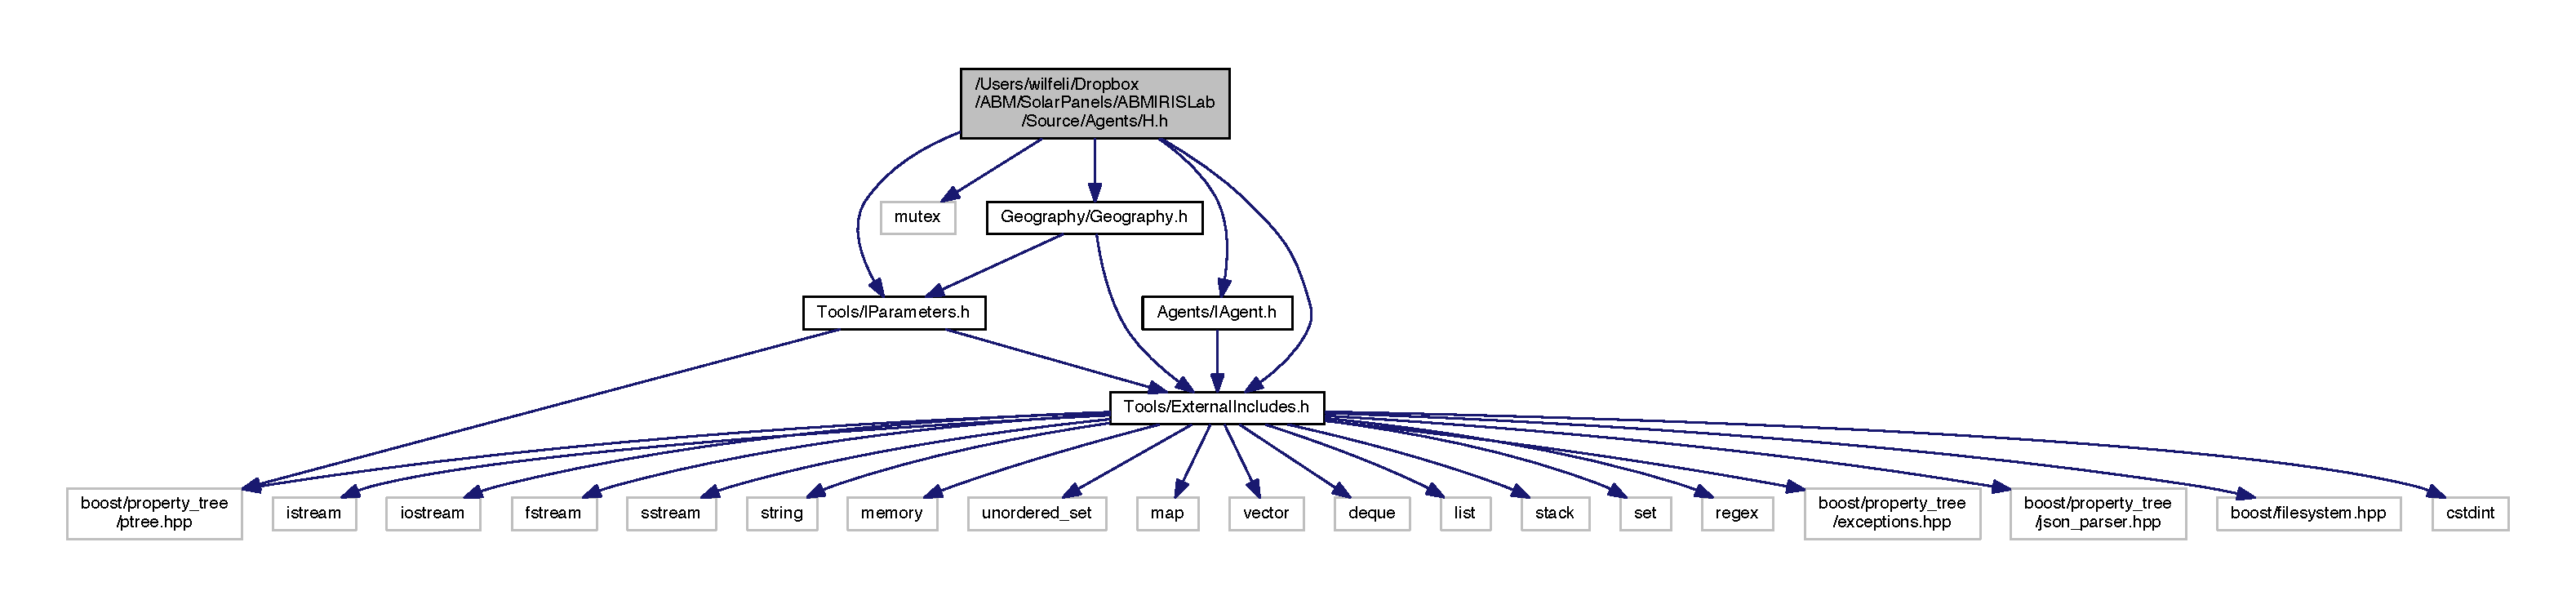
\includegraphics[width=350pt]{_h_8h__incl}
\end{center}
\end{figure}
This graph shows which files directly or indirectly include this file\+:
\nopagebreak
\begin{figure}[H]
\begin{center}
\leavevmode
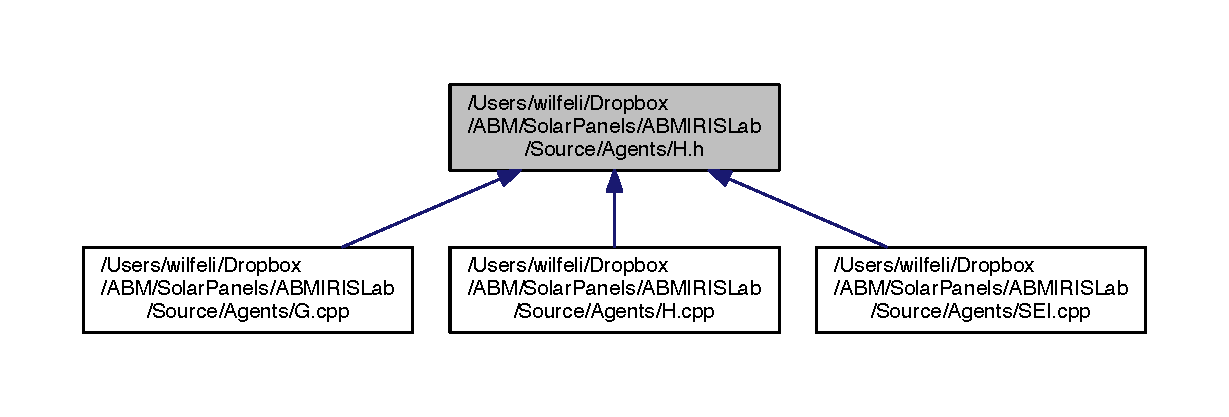
\includegraphics[width=350pt]{_h_8h__dep__incl}
\end{center}
\end{figure}
\subsection*{Classes}
\begin{DoxyCompactItemize}
\item 
class \hyperlink{classsolar__core_1_1_household}{solar\+\_\+core\+::\+Household}
\end{DoxyCompactItemize}
\subsection*{Namespaces}
\begin{DoxyCompactItemize}
\item 
 \hyperlink{namespacesolar__core}{solar\+\_\+core}
\end{DoxyCompactItemize}

\hypertarget{_s_e_i_8h}{}\section{/\+Users/wilfeli/\+Dropbox/\+A\+B\+M/\+Solar\+Panels/\+A\+B\+M\+I\+R\+I\+S\+Lab/\+Source/\+Agents/\+S\+E\+I.h File Reference}
\label{_s_e_i_8h}\index{/\+Users/wilfeli/\+Dropbox/\+A\+B\+M/\+Solar\+Panels/\+A\+B\+M\+I\+R\+I\+S\+Lab/\+Source/\+Agents/\+S\+E\+I.\+h@{/\+Users/wilfeli/\+Dropbox/\+A\+B\+M/\+Solar\+Panels/\+A\+B\+M\+I\+R\+I\+S\+Lab/\+Source/\+Agents/\+S\+E\+I.\+h}}
\subsection*{Classes}
\begin{DoxyCompactItemize}
\item 
class \hyperlink{classsolar__core_1_1_s_e_i}{solar\+\_\+core\+::\+S\+E\+I}
\end{DoxyCompactItemize}
\subsection*{Namespaces}
\begin{DoxyCompactItemize}
\item 
 \hyperlink{namespacesolar__core}{solar\+\_\+core}
\end{DoxyCompactItemize}

\hypertarget{_s_e_m_8h}{}\section{/\+Users/wilfeli/\+Dropbox/\+A\+B\+M/\+Solar\+Panels/\+A\+B\+M\+I\+R\+I\+S\+Lab/\+Source/\+Agents/\+S\+E\+M.h File Reference}
\label{_s_e_m_8h}\index{/\+Users/wilfeli/\+Dropbox/\+A\+B\+M/\+Solar\+Panels/\+A\+B\+M\+I\+R\+I\+S\+Lab/\+Source/\+Agents/\+S\+E\+M.\+h@{/\+Users/wilfeli/\+Dropbox/\+A\+B\+M/\+Solar\+Panels/\+A\+B\+M\+I\+R\+I\+S\+Lab/\+Source/\+Agents/\+S\+E\+M.\+h}}
{\ttfamily \#include \char`\"{}Tools/\+I\+Parameters.\+h\char`\"{}}\\*
{\ttfamily \#include \char`\"{}Tools/\+External\+Includes.\+h\char`\"{}}\\*
{\ttfamily \#include \char`\"{}Tools/\+I\+D.\+h\char`\"{}}\\*
Include dependency graph for S\+E\+M.\+h\+:
\nopagebreak
\begin{figure}[H]
\begin{center}
\leavevmode
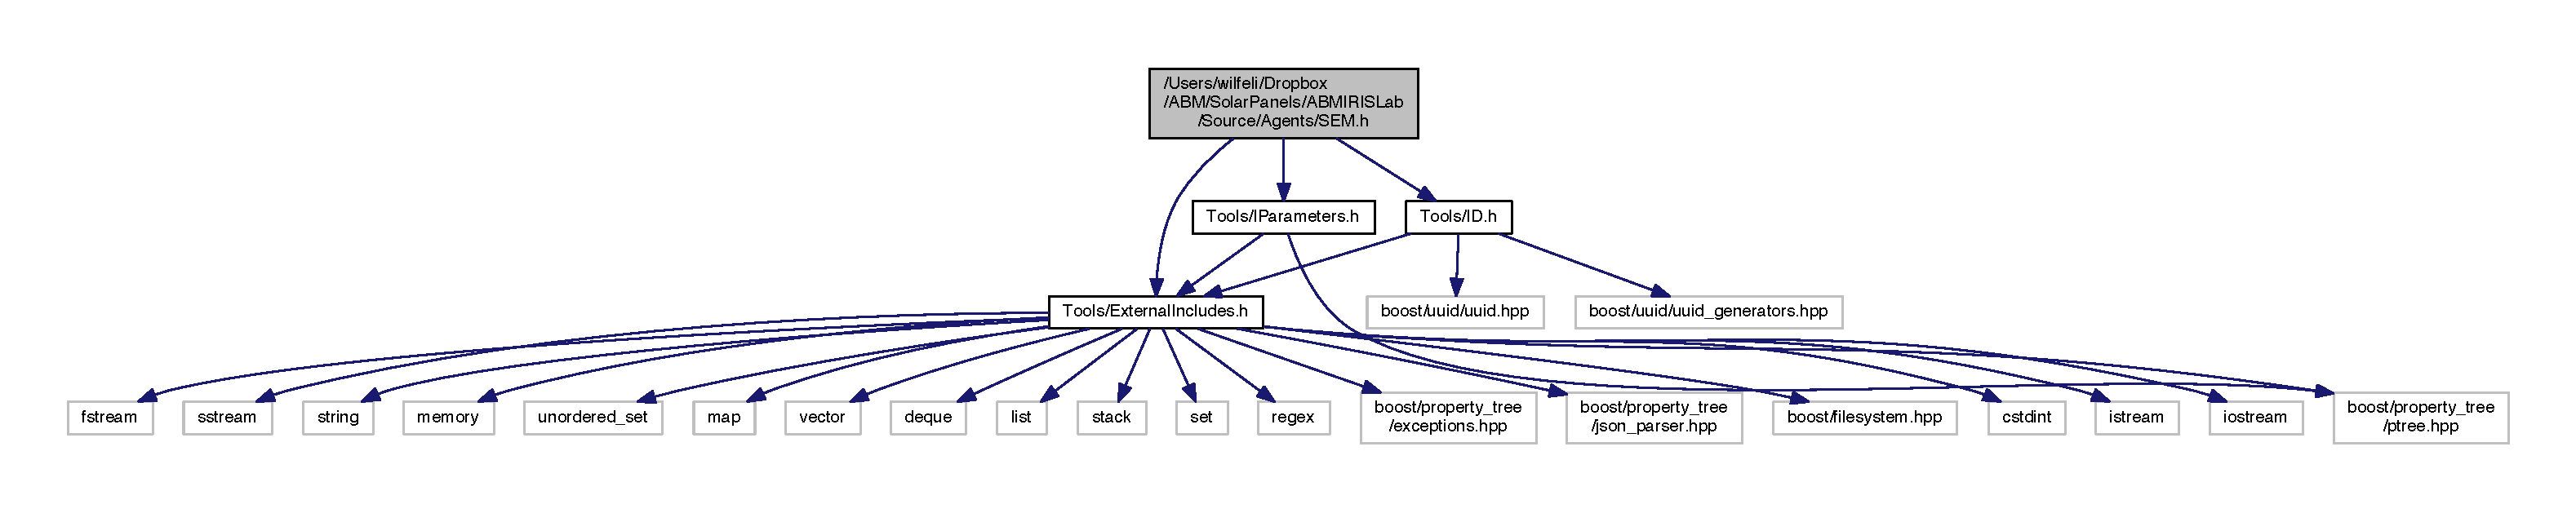
\includegraphics[width=350pt]{_s_e_m_8h__incl}
\end{center}
\end{figure}
This graph shows which files directly or indirectly include this file\+:
\nopagebreak
\begin{figure}[H]
\begin{center}
\leavevmode
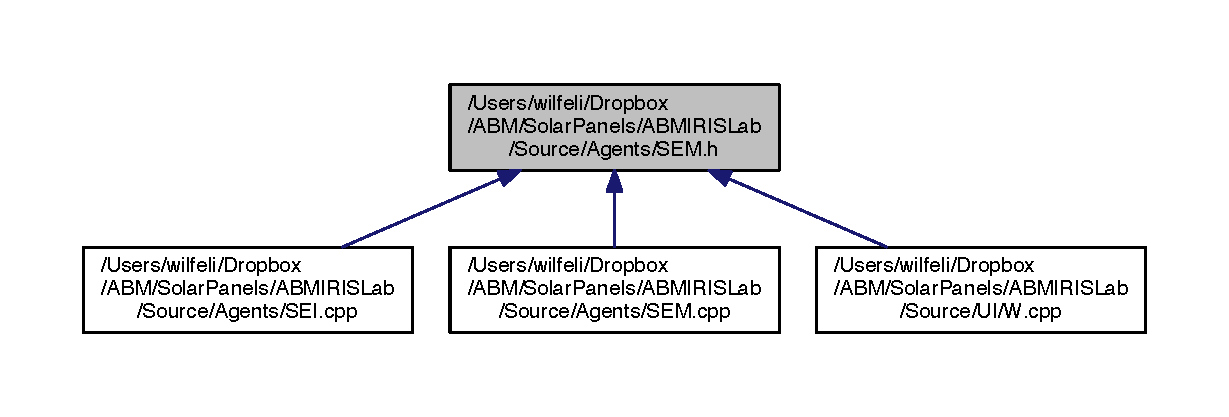
\includegraphics[width=350pt]{_s_e_m_8h__dep__incl}
\end{center}
\end{figure}
\subsection*{Classes}
\begin{DoxyCompactItemize}
\item 
class \hyperlink{classsolar__core_1_1_s_e_m}{solar\+\_\+core\+::\+S\+E\+M}
\end{DoxyCompactItemize}
\subsection*{Namespaces}
\begin{DoxyCompactItemize}
\item 
 \hyperlink{namespacesolar__core}{solar\+\_\+core}
\end{DoxyCompactItemize}

\hypertarget{_geography_8h}{}\section{/\+Users/wilfeli/\+Dropbox/\+A\+B\+M/\+Solar\+Panels/\+A\+B\+M\+I\+R\+I\+S\+Lab/\+Source/\+Geography/\+Geography.h File Reference}
\label{_geography_8h}\index{/\+Users/wilfeli/\+Dropbox/\+A\+B\+M/\+Solar\+Panels/\+A\+B\+M\+I\+R\+I\+S\+Lab/\+Source/\+Geography/\+Geography.\+h@{/\+Users/wilfeli/\+Dropbox/\+A\+B\+M/\+Solar\+Panels/\+A\+B\+M\+I\+R\+I\+S\+Lab/\+Source/\+Geography/\+Geography.\+h}}
{\ttfamily \#include $<$vector$>$}\\*
Include dependency graph for Geography.\+h\+:\nopagebreak
\begin{figure}[H]
\begin{center}
\leavevmode
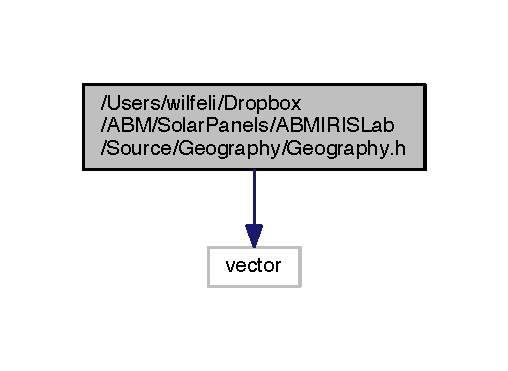
\includegraphics[width=244pt]{_geography_8h__incl}
\end{center}
\end{figure}
This graph shows which files directly or indirectly include this file\+:\nopagebreak
\begin{figure}[H]
\begin{center}
\leavevmode
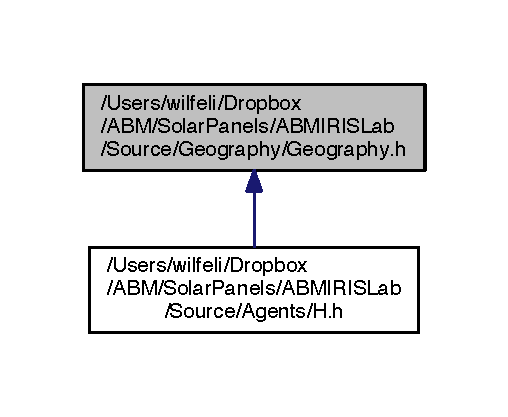
\includegraphics[width=244pt]{_geography_8h__dep__incl}
\end{center}
\end{figure}
\subsection*{Classes}
\begin{DoxyCompactItemize}
\item 
class \hyperlink{class_house}{House}
\item 
class \hyperlink{class_tile}{Tile}
\item 
class \hyperlink{class_world_map}{World\+Map}
\end{DoxyCompactItemize}

\hypertarget{_marketing_system_8h}{}\section{/\+Users/wilfeli/\+Dropbox/\+A\+B\+M/\+Solar\+Panels/\+A\+B\+M\+I\+R\+I\+S\+Lab/\+Source/\+Institutions/\+Marketing\+System.h File Reference}
\label{_marketing_system_8h}\index{/\+Users/wilfeli/\+Dropbox/\+A\+B\+M/\+Solar\+Panels/\+A\+B\+M\+I\+R\+I\+S\+Lab/\+Source/\+Institutions/\+Marketing\+System.\+h@{/\+Users/wilfeli/\+Dropbox/\+A\+B\+M/\+Solar\+Panels/\+A\+B\+M\+I\+R\+I\+S\+Lab/\+Source/\+Institutions/\+Marketing\+System.\+h}}
{\ttfamily \#include \char`\"{}Tools/\+External\+Includes.\+h\char`\"{}}\\*
{\ttfamily \#include \char`\"{}Agents/\+I\+Agent.\+h\char`\"{}}\\*
{\ttfamily \#include \char`\"{}Institutions/\+I\+Institute.\+h\char`\"{}}\\*
Include dependency graph for Marketing\+System.\+h\+:
\nopagebreak
\begin{figure}[H]
\begin{center}
\leavevmode
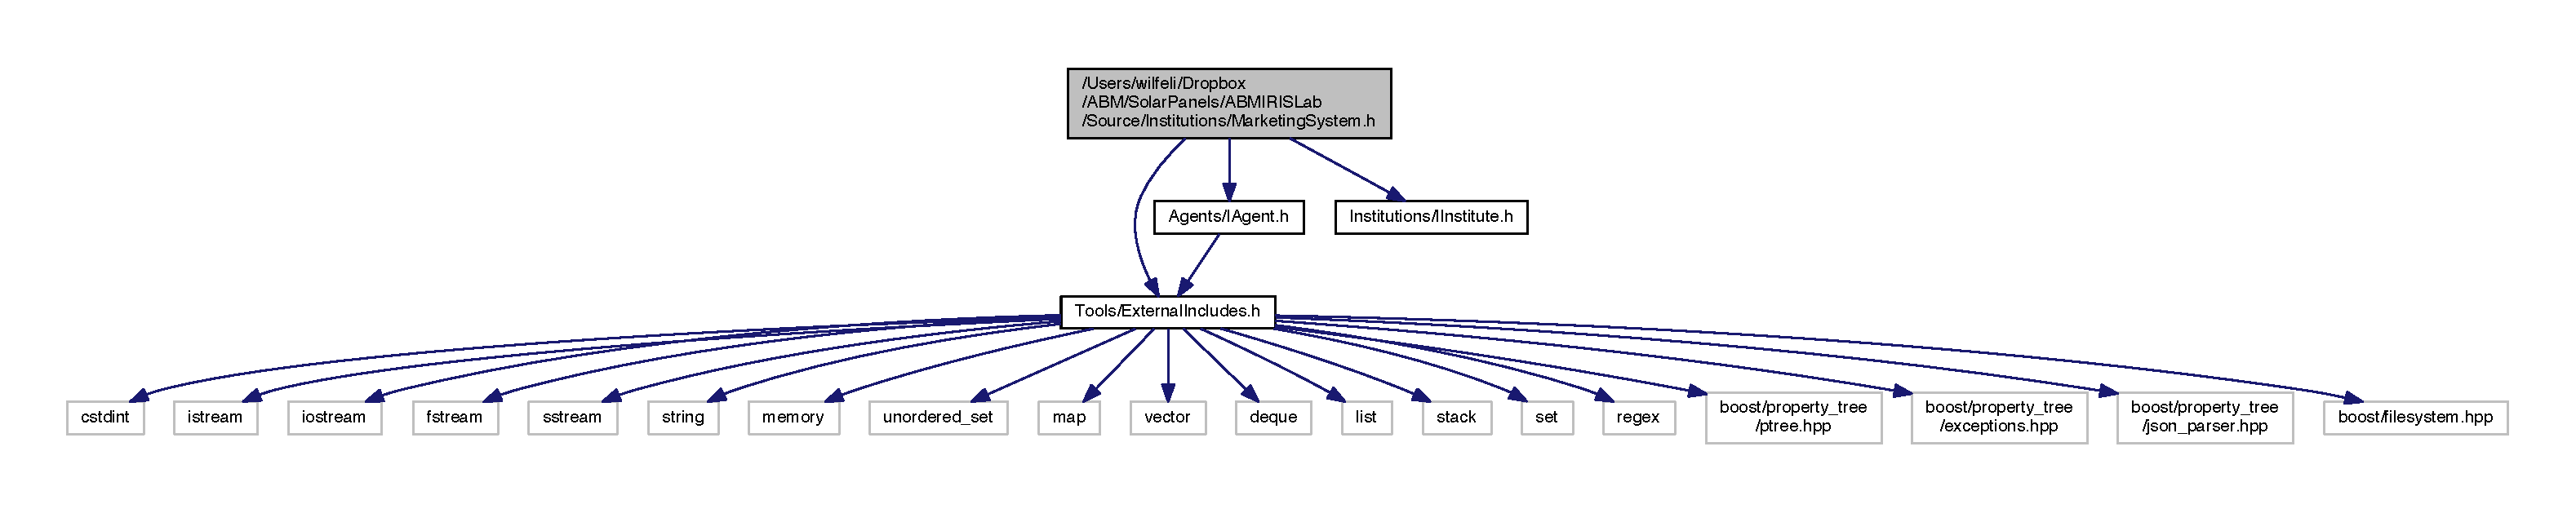
\includegraphics[width=350pt]{_marketing_system_8h__incl}
\end{center}
\end{figure}
This graph shows which files directly or indirectly include this file\+:\nopagebreak
\begin{figure}[H]
\begin{center}
\leavevmode
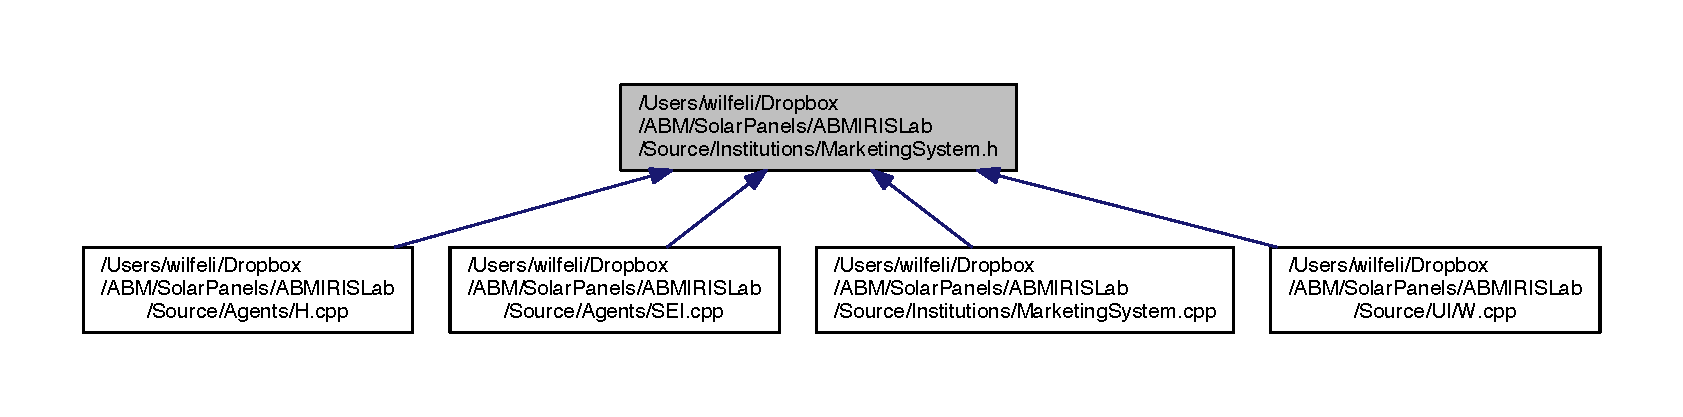
\includegraphics[width=280pt]{_marketing_system_8h__dep__incl}
\end{center}
\end{figure}
\subsection*{Classes}
\begin{DoxyCompactItemize}
\item 
class \hyperlink{classsolar__core_1_1_marketing_inst}{solar\+\_\+core\+::\+Marketing\+Inst}
\end{DoxyCompactItemize}
\subsection*{Namespaces}
\begin{DoxyCompactItemize}
\item 
 \hyperlink{namespacesolar__core}{solar\+\_\+core}
\end{DoxyCompactItemize}

\hypertarget{_documentation_8h}{}\section{/\+Users/wilfeli/\+Dropbox/\+A\+B\+M/\+Solar\+Panels/\+A\+B\+M\+I\+R\+I\+S\+Lab/\+Source/\+Tools/\+Documentation.h File Reference}
\label{_documentation_8h}\index{/\+Users/wilfeli/\+Dropbox/\+A\+B\+M/\+Solar\+Panels/\+A\+B\+M\+I\+R\+I\+S\+Lab/\+Source/\+Tools/\+Documentation.\+h@{/\+Users/wilfeli/\+Dropbox/\+A\+B\+M/\+Solar\+Panels/\+A\+B\+M\+I\+R\+I\+S\+Lab/\+Source/\+Tools/\+Documentation.\+h}}

\hypertarget{_i_parameters_8h}{}\section{/\+Users/wilfeli/\+Dropbox/\+A\+B\+M/\+Solar\+Panels/\+A\+B\+M\+I\+R\+I\+S\+Lab/\+Source/\+Tools/\+I\+Parameters.h File Reference}
\label{_i_parameters_8h}\index{/\+Users/wilfeli/\+Dropbox/\+A\+B\+M/\+Solar\+Panels/\+A\+B\+M\+I\+R\+I\+S\+Lab/\+Source/\+Tools/\+I\+Parameters.\+h@{/\+Users/wilfeli/\+Dropbox/\+A\+B\+M/\+Solar\+Panels/\+A\+B\+M\+I\+R\+I\+S\+Lab/\+Source/\+Tools/\+I\+Parameters.\+h}}
{\ttfamily \#include \char`\"{}Tools/\+External\+Includes.\+h\char`\"{}}\\*
{\ttfamily \#include $<$boost/property\+\_\+tree/ptree.\+hpp$>$}\\*
Include dependency graph for I\+Parameters.\+h\+:
\nopagebreak
\begin{figure}[H]
\begin{center}
\leavevmode
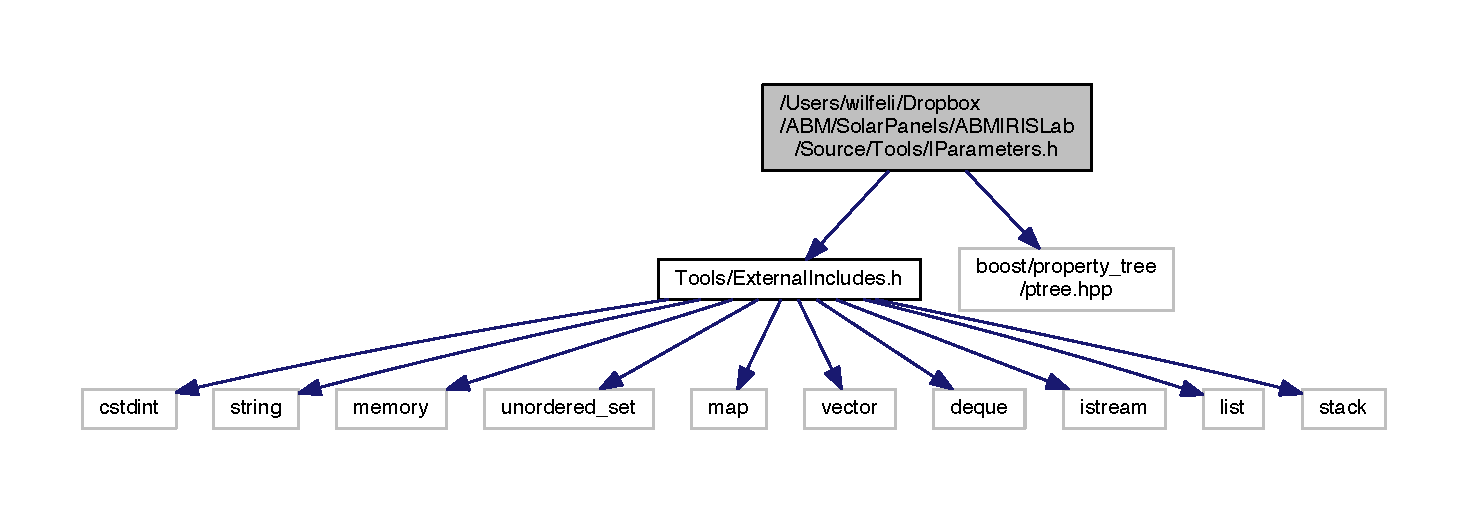
\includegraphics[width=350pt]{_i_parameters_8h__incl}
\end{center}
\end{figure}
This graph shows which files directly or indirectly include this file\+:
\nopagebreak
\begin{figure}[H]
\begin{center}
\leavevmode
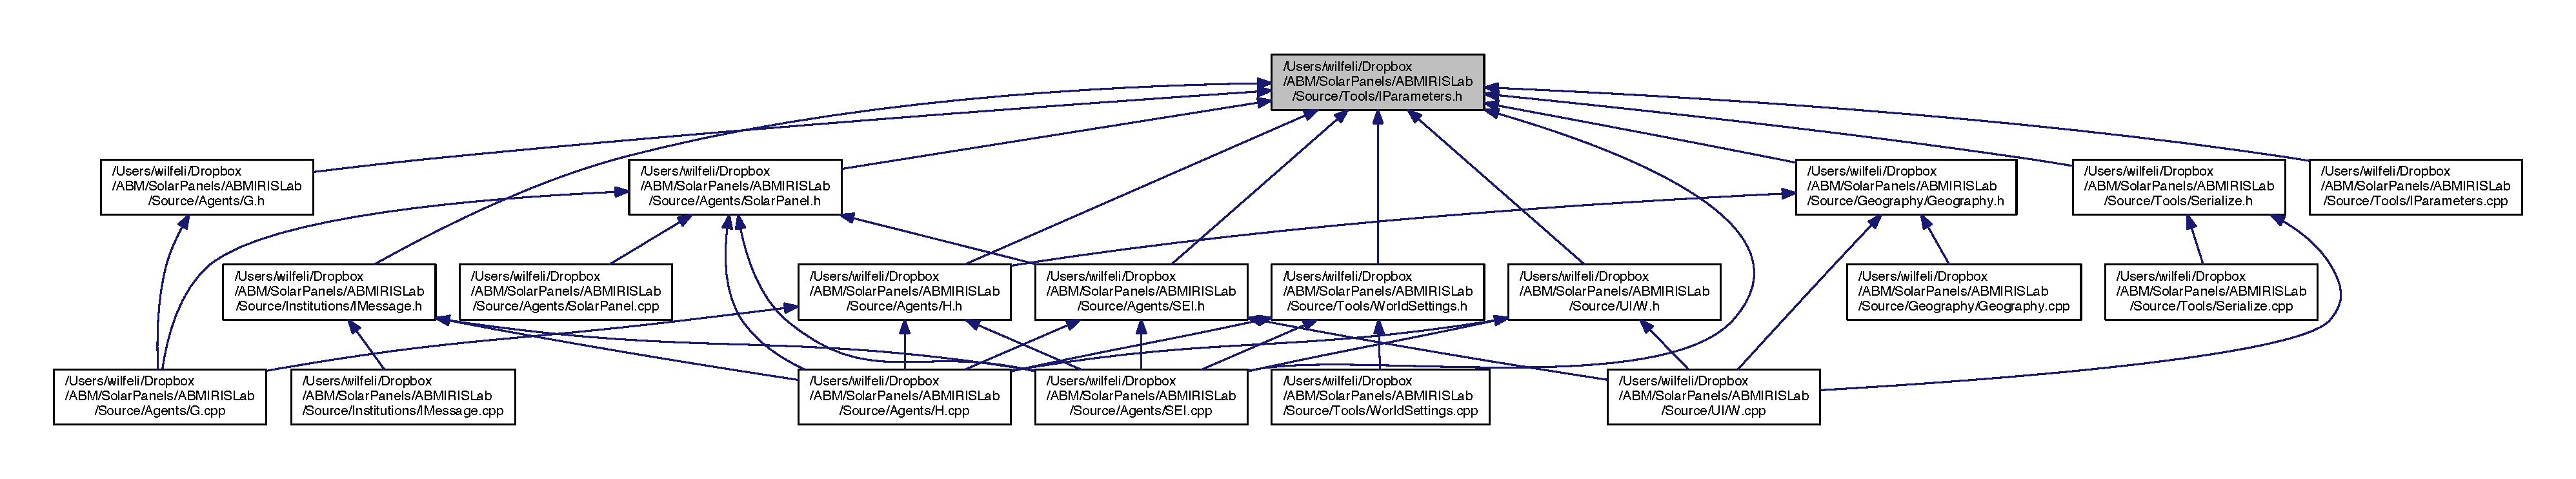
\includegraphics[width=350pt]{_i_parameters_8h__dep__incl}
\end{center}
\end{figure}
\subsection*{Classes}
\begin{DoxyCompactItemize}
\item 
class \hyperlink{classsolar__core_1_1_enum_factory}{solar\+\_\+core\+::\+Enum\+Factory}
\end{DoxyCompactItemize}
\subsection*{Namespaces}
\begin{DoxyCompactItemize}
\item 
 \hyperlink{namespacesolar__core}{solar\+\_\+core}
\item 
 \hyperlink{namespacesolar__core_1_1constants}{solar\+\_\+core\+::constants}
\end{DoxyCompactItemize}
\subsection*{Typedefs}
\begin{DoxyCompactItemize}
\item 
typedef int64\+\_\+t \hyperlink{namespacesolar__core_a4b5949d07259da6f8a20d12a30403e90}{solar\+\_\+core\+::\+Time\+Unit}
\item 
typedef boost\+::property\+\_\+tree\+::ptree \hyperlink{namespacesolar__core_adeda2737d6938c190eb774a5b2495045}{solar\+\_\+core\+::\+Property\+Tree}
\item 
typedef std\+::underlying\+\_\+type$<$ E\+Param\+Types $>$\+::type \hyperlink{namespacesolar__core_a256e8e2dc052f522b522d3f90b294caf}{solar\+\_\+core\+::\+E\+Param\+Types\+\_\+type}
\end{DoxyCompactItemize}
\subsection*{Enumerations}
\begin{DoxyCompactItemize}
\item 
enum \hyperlink{namespacesolar__core_aa1147341e5ef7a40d68d1bd68e149362}{solar\+\_\+core\+::\+E\+Param\+Types} \+: int64\+\_\+t \{ \\*
\hyperlink{namespacesolar__core_aa1147341e5ef7a40d68d1bd68e149362a1f08d08fd864b99cbeebd88b9a0784a7}{solar\+\_\+core\+::\+E\+Param\+Types\+::\+Income}, 
\hyperlink{namespacesolar__core_aa1147341e5ef7a40d68d1bd68e149362a62c5cc90270449db38e6fb4f2db71c55}{solar\+\_\+core\+::\+E\+Param\+Types\+::\+N\+\_\+\+H}, 
\hyperlink{namespacesolar__core_aa1147341e5ef7a40d68d1bd68e149362a417bef7b89fce8abf638b9983a79a70e}{solar\+\_\+core\+::\+E\+Param\+Types\+::\+Credit\+Score}, 
\hyperlink{namespacesolar__core_aa1147341e5ef7a40d68d1bd68e149362a9b8cd62150c419c61129f736404b0579}{solar\+\_\+core\+::\+E\+Param\+Types\+::\+Electricity\+Bill}, 
\\*
\hyperlink{namespacesolar__core_aa1147341e5ef7a40d68d1bd68e149362a2bf6593af19bb602f7c596d7327c6dd6}{solar\+\_\+core\+::\+E\+Param\+Types\+::\+Roof\+Size}, 
\hyperlink{namespacesolar__core_aa1147341e5ef7a40d68d1bd68e149362abff61b25127aa53b8eb7343edf48166b}{solar\+\_\+core\+::\+E\+Param\+Types\+::\+Roof\+Age}, 
\hyperlink{namespacesolar__core_aa1147341e5ef7a40d68d1bd68e149362afc91168d2e624505b0168a1ee8c0c60e}{solar\+\_\+core\+::\+E\+Param\+Types\+::\+H\+H\+Marketing\+State\+Highly\+Interested}, 
\hyperlink{namespacesolar__core_aa1147341e5ef7a40d68d1bd68e149362a985f6ff4deb35454155c9e992bfcdbb0}{solar\+\_\+core\+::\+E\+Param\+Types\+::\+H\+H\+Marketing\+State\+Interested}, 
\\*
\hyperlink{namespacesolar__core_aa1147341e5ef7a40d68d1bd68e149362ab970e992ff02930a86716c0390fa42df}{solar\+\_\+core\+::\+E\+Param\+Types\+::\+H\+H\+Marketing\+Not\+Interested}, 
\hyperlink{namespacesolar__core_aa1147341e5ef7a40d68d1bd68e149362a5a8012f218ced859bad78be09e8e46e7}{solar\+\_\+core\+::\+E\+Param\+Types\+::\+Active\+Quoting}, 
\hyperlink{namespacesolar__core_aa1147341e5ef7a40d68d1bd68e149362a31ead751600c8439e0897f8dc736154b}{solar\+\_\+core\+::\+E\+Param\+Types\+::\+Inactive\+Quoting}, 
\hyperlink{namespacesolar__core_aa1147341e5ef7a40d68d1bd68e149362a374a1855dae7569f1de9514f0cdf09f5}{solar\+\_\+core\+::\+E\+Param\+Types\+::\+H\+H\+Decision\+Reroof}, 
\\*
\hyperlink{namespacesolar__core_aa1147341e5ef7a40d68d1bd68e149362a4580119737f0c25977ece80cbac3d58b}{solar\+\_\+core\+::\+E\+Param\+Types\+::\+H\+H\+Max\+N\+Visits\+Per\+Time\+Unit}, 
\hyperlink{namespacesolar__core_aa1147341e5ef7a40d68d1bd68e149362a619c634adba7a1386122c22d8d2021df}{solar\+\_\+core\+::\+E\+Param\+Types\+::\+H\+H\+Dec\+Preliminary\+Quote}, 
\hyperlink{namespacesolar__core_aa1147341e5ef7a40d68d1bd68e149362a91a0e5bcf4376200527bfe2b00d1ae6c}{solar\+\_\+core\+::\+E\+Param\+Types\+::\+Requested\+Online\+Quote}, 
<<<<<<< HEAD
\hyperlink{namespacesolar__core_aa1147341e5ef7a40d68d1bd68e149362a3f1645b895f679824026ca1de865ca81}{solar\+\_\+core\+::\+E\+Param\+Types\+::\+Requested\+Preliminary\+Quote}, 
\\*
\hyperlink{namespacesolar__core_aa1147341e5ef7a40d68d1bd68e149362a5d1561cc7b77d4e0eaca8cc37a4331e9}{solar\+\_\+core\+::\+E\+Param\+Types\+::\+Provided\+Online\+Quote}, 
\hyperlink{namespacesolar__core_aa1147341e5ef7a40d68d1bd68e149362ac3d9027c79b1821115c110ce9b706383}{solar\+\_\+core\+::\+E\+Param\+Types\+::\+Provided\+Preliminary\+Quote}, 
\hyperlink{namespacesolar__core_aa1147341e5ef7a40d68d1bd68e149362a6f85c2280e06a0a94e796e2c6dfbfce2}{solar\+\_\+core\+::\+E\+Param\+Types\+::\+Scheduled\+First\+Site\+Visit}, 
\hyperlink{namespacesolar__core_aa1147341e5ef7a40d68d1bd68e149362a1944aa6a68e41524b170bb07ba22fb54}{solar\+\_\+core\+::\+E\+Param\+Types\+::\+Collected\+Inf\+First\+Site\+Visit}, 
\\*
\hyperlink{namespacesolar__core_aa1147341e5ef7a40d68d1bd68e149362a94beae8137095b64c636645a10f779a9}{solar\+\_\+core\+::\+E\+Param\+Types\+::\+Required\+H\+H\+Reroof}, 
\hyperlink{namespacesolar__core_aa1147341e5ef7a40d68d1bd68e149362a7a0186947edeb230395b02fc6f9a8c37}{solar\+\_\+core\+::\+E\+Param\+Types\+::\+Waiting\+H\+H\+Reroof}, 
\hyperlink{namespacesolar__core_aa1147341e5ef7a40d68d1bd68e149362ae04bb6f7c490d1f5e1e19b790ac4bd48}{solar\+\_\+core\+::\+E\+Param\+Types\+::\+Accepted\+Preliminary\+Quote}, 
\hyperlink{namespacesolar__core_aa1147341e5ef7a40d68d1bd68e149362a8662266053d427b356392cc9fdff7b5e}{solar\+\_\+core\+::\+E\+Param\+Types\+::\+Drafted\+Design}, 
\\*
\hyperlink{namespacesolar__core_aa1147341e5ef7a40d68d1bd68e149362acc5c79b9e52a3187a8b3bfdf7796f6e5}{solar\+\_\+core\+::\+E\+Param\+Types\+::\+Accepted\+Design}, 
\hyperlink{namespacesolar__core_aa1147341e5ef7a40d68d1bd68e149362aca58ef2d2dad5072c87d596308db83d0}{solar\+\_\+core\+::\+E\+Param\+Types\+::\+Requested\+Permit}, 
\hyperlink{namespacesolar__core_aa1147341e5ef7a40d68d1bd68e149362ac94e40a26296afb13a3493d00eb8303d}{solar\+\_\+core\+::\+E\+Param\+Types\+::\+Scheduled\+Permit\+Visit}, 
\hyperlink{namespacesolar__core_aa1147341e5ef7a40d68d1bd68e149362aeb03d3042b95f0913a2646ec6d9a6ec4}{solar\+\_\+core\+::\+E\+Param\+Types\+::\+Collected\+Inf\+Permit\+Visit}, 
\\*
\hyperlink{namespacesolar__core_aa1147341e5ef7a40d68d1bd68e149362a1246349928f17a03f4bc9fc73929013a}{solar\+\_\+core\+::\+E\+Param\+Types\+::\+Scheduled\+Installation}, 
\hyperlink{namespacesolar__core_aa1147341e5ef7a40d68d1bd68e149362afd25fc3a551ab850c92076e52142705c}{solar\+\_\+core\+::\+E\+Param\+Types\+::\+Schedule\+Installation}, 
\hyperlink{namespacesolar__core_aa1147341e5ef7a40d68d1bd68e149362a84b4af953e4b4f4bcc1af7105e43cfaf}{solar\+\_\+core\+::\+E\+Param\+Types\+::\+Pending\+Materials}, 
\hyperlink{namespacesolar__core_aa1147341e5ef7a40d68d1bd68e149362a98dd43dfae05b11befe1f140e0ec787a}{solar\+\_\+core\+::\+E\+Param\+Types\+::\+Installed}, 
\\*
\hyperlink{namespacesolar__core_aa1147341e5ef7a40d68d1bd68e149362a62e7c876fbc842b593d4473c0ae28521}{solar\+\_\+core\+::\+E\+Param\+Types\+::\+Requested\+Permit\+For\+Installation}, 
\hyperlink{namespacesolar__core_aa1147341e5ef7a40d68d1bd68e149362afe8a13c6d0eddf9ed3a0686bf03fb5dc}{solar\+\_\+core\+::\+E\+Param\+Types\+::\+Granted\+Permit\+For\+Installation}, 
\hyperlink{namespacesolar__core_aa1147341e5ef7a40d68d1bd68e149362afad1d49bf654e94e0db269cbf0d6dc5e}{solar\+\_\+core\+::\+E\+Param\+Types\+::\+Requested\+Inspection\+After\+Installation}, 
\hyperlink{namespacesolar__core_aa1147341e5ef7a40d68d1bd68e149362a95e2095019cb1db25213fde329af40a3}{solar\+\_\+core\+::\+E\+Param\+Types\+::\+Passed\+Inspection\+After\+Installation}, 
\\*
\hyperlink{namespacesolar__core_aa1147341e5ef7a40d68d1bd68e149362a5437744a7fb1f45fdf5d109c4444e7d6}{solar\+\_\+core\+::\+E\+Param\+Types\+::\+Requested\+Permit\+For\+Interconnection}, 
\hyperlink{namespacesolar__core_aa1147341e5ef7a40d68d1bd68e149362af915b5ae43a4c3adc79b2ce7d6e3a679}{solar\+\_\+core\+::\+E\+Param\+Types\+::\+Granted\+Permit\+For\+Interconnection}, 
=======
\hyperlink{namespacesolar__core_aa1147341e5ef7a40d68d1bd68e149362a6d84e672f96624f4c6323a7543a5de1f}{solar\+\_\+core\+::\+E\+Param\+Types\+::\+Request\+Preliminary\+Quote}, 
\\*
\hyperlink{namespacesolar__core_aa1147341e5ef7a40d68d1bd68e149362a3f1645b895f679824026ca1de865ca81}{solar\+\_\+core\+::\+E\+Param\+Types\+::\+Requested\+Preliminary\+Quote}, 
\hyperlink{namespacesolar__core_aa1147341e5ef7a40d68d1bd68e149362a5d1561cc7b77d4e0eaca8cc37a4331e9}{solar\+\_\+core\+::\+E\+Param\+Types\+::\+Provided\+Online\+Quote}, 
\hyperlink{namespacesolar__core_aa1147341e5ef7a40d68d1bd68e149362ac3d9027c79b1821115c110ce9b706383}{solar\+\_\+core\+::\+E\+Param\+Types\+::\+Provided\+Preliminary\+Quote}, 
\hyperlink{namespacesolar__core_aa1147341e5ef7a40d68d1bd68e149362a6f85c2280e06a0a94e796e2c6dfbfce2}{solar\+\_\+core\+::\+E\+Param\+Types\+::\+Scheduled\+First\+Site\+Visit}, 
\\*
\hyperlink{namespacesolar__core_aa1147341e5ef7a40d68d1bd68e149362a1944aa6a68e41524b170bb07ba22fb54}{solar\+\_\+core\+::\+E\+Param\+Types\+::\+Collected\+Inf\+First\+Site\+Visit}, 
\hyperlink{namespacesolar__core_aa1147341e5ef7a40d68d1bd68e149362a94beae8137095b64c636645a10f779a9}{solar\+\_\+core\+::\+E\+Param\+Types\+::\+Required\+H\+H\+Reroof}, 
\hyperlink{namespacesolar__core_aa1147341e5ef7a40d68d1bd68e149362a7a0186947edeb230395b02fc6f9a8c37}{solar\+\_\+core\+::\+E\+Param\+Types\+::\+Waiting\+H\+H\+Reroof}, 
\hyperlink{namespacesolar__core_aa1147341e5ef7a40d68d1bd68e149362ae04bb6f7c490d1f5e1e19b790ac4bd48}{solar\+\_\+core\+::\+E\+Param\+Types\+::\+Accepted\+Preliminary\+Quote}, 
\\*
\hyperlink{namespacesolar__core_aa1147341e5ef7a40d68d1bd68e149362a8662266053d427b356392cc9fdff7b5e}{solar\+\_\+core\+::\+E\+Param\+Types\+::\+Drafted\+Design}, 
\hyperlink{namespacesolar__core_aa1147341e5ef7a40d68d1bd68e149362acc5c79b9e52a3187a8b3bfdf7796f6e5}{solar\+\_\+core\+::\+E\+Param\+Types\+::\+Accepted\+Design}, 
\hyperlink{namespacesolar__core_aa1147341e5ef7a40d68d1bd68e149362aca58ef2d2dad5072c87d596308db83d0}{solar\+\_\+core\+::\+E\+Param\+Types\+::\+Requested\+Permit}, 
\hyperlink{namespacesolar__core_aa1147341e5ef7a40d68d1bd68e149362a9a4ff00bed0dd4c2cbcd986eb71654b5}{solar\+\_\+core\+::\+E\+Param\+Types\+::\+Granted\+Permit}, 
\\*
\hyperlink{namespacesolar__core_aa1147341e5ef7a40d68d1bd68e149362a1246349928f17a03f4bc9fc73929013a}{solar\+\_\+core\+::\+E\+Param\+Types\+::\+Scheduled\+Installation}, 
\hyperlink{namespacesolar__core_aa1147341e5ef7a40d68d1bd68e149362a98dd43dfae05b11befe1f140e0ec787a}{solar\+\_\+core\+::\+E\+Param\+Types\+::\+Installed}, 
>>>>>>> 9fadf023062505cb443534457ab9d4d3cc1b7bfc
\hyperlink{namespacesolar__core_aa1147341e5ef7a40d68d1bd68e149362a36011ab25e125345f76caf5e8f027175}{solar\+\_\+core\+::\+E\+Param\+Types\+::\+Closed\+Project}, 
\hyperlink{namespacesolar__core_aa1147341e5ef7a40d68d1bd68e149362ac2c46b3ff478ae34297f8672b3d91497}{solar\+\_\+core\+::\+E\+Param\+Types\+::\+Online\+Quote\+Price}, 
\\*
\hyperlink{namespacesolar__core_aa1147341e5ef7a40d68d1bd68e149362a9cdd993b8d48601635f529f0e4d93299}{solar\+\_\+core\+::\+E\+Param\+Types\+::\+Online\+Quote\+Estimated\+Savings}, 
\hyperlink{namespacesolar__core_aa1147341e5ef7a40d68d1bd68e149362a581329dc30b846b1b05267c8bbfb3dc2}{solar\+\_\+core\+::\+E\+Param\+Types\+::\+Preliminary\+Quote\+Price}, 
\hyperlink{namespacesolar__core_aa1147341e5ef7a40d68d1bd68e149362ac9882efbffdf2ae9422abfc3e4d4a032}{solar\+\_\+core\+::\+E\+Param\+Types\+::\+Preliminary\+Quote\+Estimated\+Savings}, 
\hyperlink{namespacesolar__core_aa1147341e5ef7a40d68d1bd68e149362a65e9babf589ac04a35221b97b0449611}{solar\+\_\+core\+::\+E\+Param\+Types\+::\+Estimated\+Price\+Per\+Watt}, 
\\*
\hyperlink{namespacesolar__core_aa1147341e5ef7a40d68d1bd68e149362a00420d47e5664414646cd5cc5245c914}{solar\+\_\+core\+::\+E\+Param\+Types\+::\+Average\+P\+V\+Price}, 
\hyperlink{namespacesolar__core_aa1147341e5ef7a40d68d1bd68e149362ab820b21cf6b896d9ffe4f3180344aaad}{solar\+\_\+core\+::\+E\+Param\+Types\+::\+Average\+P\+V\+Capacity}, 
\hyperlink{namespacesolar__core_aa1147341e5ef7a40d68d1bd68e149362a95318d634060f210ca2cbc8487913a23}{solar\+\_\+core\+::\+E\+Param\+Types\+::\+Electricity\+Price\+U\+C\+Demand}, 
\hyperlink{namespacesolar__core_aa1147341e5ef7a40d68d1bd68e149362a57bd39ffa6aea05e5ffe8481417466f8}{solar\+\_\+core\+::\+E\+Param\+Types\+::\+Electricity\+Price\+U\+C\+Supply}, 
\\*
\hyperlink{namespacesolar__core_aa1147341e5ef7a40d68d1bd68e149362a7f416fbc5b5a75a37caa766533274218}{solar\+\_\+core\+::\+E\+Param\+Types\+::\+Inflation\+Rate}, 
\hyperlink{namespacesolar__core_aa1147341e5ef7a40d68d1bd68e149362ab49cdbc17a92df4982fae394c33aac83}{solar\+\_\+core\+::\+E\+Param\+Types\+::\+D\+Cto\+A\+C\+Loss}, 
<<<<<<< HEAD
\hyperlink{namespacesolar__core_aa1147341e5ef7a40d68d1bd68e149362a0aa925df388c8a6dc119a25298b58831}{solar\+\_\+core\+::\+E\+Param\+Types\+::\+Degradation\+Definition\+Length}, 
=======
>>>>>>> 9fadf023062505cb443534457ab9d4d3cc1b7bfc
\hyperlink{namespacesolar__core_aa1147341e5ef7a40d68d1bd68e149362a2b772976cb89ca861f4a970d8eed2959}{solar\+\_\+core\+::\+E\+Param\+Types\+::\+S\+E\+I\+Small}, 
\\*
\hyperlink{namespacesolar__core_aa1147341e5ef7a40d68d1bd68e149362a827914969a84c51a2e5722d05a311c97}{solar\+\_\+core\+::\+E\+Param\+Types\+::\+S\+E\+I\+Large}, 
<<<<<<< HEAD
\hyperlink{namespacesolar__core_aa1147341e5ef7a40d68d1bd68e149362a159b446def618d2defa97ad1818ad6dc}{solar\+\_\+core\+::\+E\+Param\+Types\+::\+S\+E\+I\+Processing\+Time\+Required\+For\+Preliminary\+Quote}, 
\hyperlink{namespacesolar__core_aa1147341e5ef7a40d68d1bd68e149362aee8260c2afdde8270a04e738d6dfd61e}{solar\+\_\+core\+::\+E\+Param\+Types\+::\+S\+E\+I\+Processing\+Time\+Required\+For\+Scheduling\+First\+Site\+Visit}, 
\hyperlink{namespacesolar__core_aa1147341e5ef7a40d68d1bd68e149362a21df8a580ed978b021e23a928d19b29e}{solar\+\_\+core\+::\+E\+Param\+Types\+::\+S\+E\+I\+Processing\+Time\+Required\+For\+Design}, 
\\*
\hyperlink{namespacesolar__core_aa1147341e5ef7a40d68d1bd68e149362ad6e334fa57e5846cf4ba4b182dadca1d}{solar\+\_\+core\+::\+E\+Param\+Types\+::\+S\+E\+I\+Max\+N\+Visits\+Per\+Time\+Unit}, 
\hyperlink{namespacesolar__core_aa1147341e5ef7a40d68d1bd68e149362acd42418f4ce0736c05d2aa8b36694774}{solar\+\_\+core\+::\+E\+Param\+Types\+::\+S\+E\+I\+Max\+N\+Installations\+Per\+Time\+Unit}, 
\hyperlink{namespacesolar__core_aa1147341e5ef7a40d68d1bd68e149362a79d36b9c925b7e55309fd4436f67c4ee}{solar\+\_\+core\+::\+E\+Param\+Types\+::\+S\+E\+I\+Max\+Roof\+Age}, 
\hyperlink{namespacesolar__core_aa1147341e5ef7a40d68d1bd68e149362ae48d553d39bcd7d207890c610fa1e74c}{solar\+\_\+core\+::\+E\+Param\+Types\+::\+S\+E\+I\+Frequency\+Update\+Design\+Templates}, 
\\*
\hyperlink{namespacesolar__core_aa1147341e5ef7a40d68d1bd68e149362ad03dae753c26cb012acd3a7dcd41dc8c}{solar\+\_\+core\+::\+E\+Param\+Types\+::\+S\+E\+I\+High\+Efficiency\+Design}, 
\hyperlink{namespacesolar__core_aa1147341e5ef7a40d68d1bd68e149362a2b4390775acd3d31e3049d242a1dd196}{solar\+\_\+core\+::\+E\+Param\+Types\+::\+S\+E\+I\+Mid\+Efficiency\+Design}, 
\hyperlink{namespacesolar__core_aa1147341e5ef7a40d68d1bd68e149362ab2592ca389b1a29cf91ddefe8d6769a2}{solar\+\_\+core\+::\+E\+Param\+Types\+::\+S\+E\+I\+Low\+Efficiency\+Design}, 
\hyperlink{namespacesolar__core_aa1147341e5ef7a40d68d1bd68e149362ad82c5bc04656736eec60bb0ae5cc1c86}{solar\+\_\+core\+::\+E\+Param\+Types\+::\+S\+E\+M\+Frequency\+Production}, 
\\*
\hyperlink{namespacesolar__core_aa1147341e5ef7a40d68d1bd68e149362a34756d8af48afa073b9b1a99c343eaf8}{solar\+\_\+core\+::\+E\+Param\+Types\+::\+S\+E\+M\+Production\+Quantity}, 
\hyperlink{namespacesolar__core_aa1147341e5ef7a40d68d1bd68e149362ac04aa42bb11a9e4ac99570dea8ff6ccb}{solar\+\_\+core\+::\+E\+Param\+Types\+::\+S\+E\+M\+Frequency\+Research\+Templates}, 
\hyperlink{namespacesolar__core_aa1147341e5ef7a40d68d1bd68e149362ae758a4ed2eec01e6e3fd3a88f04879db}{solar\+\_\+core\+::\+E\+Param\+Types\+::\+S\+E\+M\+N\+Solar\+Panels\+Research}, 
\hyperlink{namespacesolar__core_aa1147341e5ef7a40d68d1bd68e149362a9624aa5f0b1cb060f06e659e6ad0bb32}{solar\+\_\+core\+::\+E\+Param\+Types\+::\+S\+E\+M\+Efficiency\+Upgrade\+Research}, 
\\*
\hyperlink{namespacesolar__core_aa1147341e5ef7a40d68d1bd68e149362acd0c33f5dd54f7b8969a1abe3fff6395}{solar\+\_\+core\+::\+E\+Param\+Types\+::\+S\+E\+M\+Frequency\+Price\+Decisions}, 
\hyperlink{namespacesolar__core_aa1147341e5ef7a40d68d1bd68e149362a6dcf74cc979e2b36553e512f5d945dda}{solar\+\_\+core\+::\+E\+Param\+Types\+::\+S\+E\+M\+Price\+Base\+Efficiency}, 
\hyperlink{namespacesolar__core_aa1147341e5ef7a40d68d1bd68e149362a378a3f0391921c61ec958fd2ff297533}{solar\+\_\+core\+::\+E\+Param\+Types\+::\+S\+E\+M\+Price\+Markup\+Efficiency}, 
\hyperlink{namespacesolar__core_aa1147341e5ef7a40d68d1bd68e149362a67c3e4e1576f6ca5335ad02183c045d9}{solar\+\_\+core\+::\+E\+Param\+Types\+::\+G\+Processing\+Time\+Required\+For\+Scheduling\+Permit\+Visit}, 
\\*
\hyperlink{namespacesolar__core_aa1147341e5ef7a40d68d1bd68e149362a7b4067a4358525ace9b7673fe62412d7}{solar\+\_\+core\+::\+E\+Param\+Types\+::\+G\+Max\+N\+Visits\+Per\+Time\+Unit}, 
\hyperlink{namespacesolar__core_aa1147341e5ef7a40d68d1bd68e149362abc0e6872c4d8b9e3f47fa58db0cbf5b7}{solar\+\_\+core\+::\+E\+Param\+Types\+::\+G\+Processing\+Time\+Required\+For\+Processing\+Permit}, 
\hyperlink{namespacesolar__core_aa1147341e5ef7a40d68d1bd68e149362a6333f5438608185430ed6a4320c9624b}{solar\+\_\+core\+::\+E\+Param\+Types\+::\+G\+Processing\+Time\+Required\+For\+Granting\+Permit\+For\+Installation}, 
\hyperlink{namespacesolar__core_aa1147341e5ef7a40d68d1bd68e149362a07eca072965a434d37bad8ecedd352d2}{solar\+\_\+core\+::\+E\+Param\+Types\+::\+Utility\+Processing\+Time\+Required\+For\+Permit}, 
\\*
\hyperlink{namespacesolar__core_aa1147341e5ef7a40d68d1bd68e149362a3f69bebe61422371b4b411bdaa9486fb}{solar\+\_\+core\+::\+E\+Param\+Types\+::\+Utility\+Max\+Capacity}, 
\hyperlink{namespacesolar__core_aa1147341e5ef7a40d68d1bd68e149362ae5a11f9f2a59691e2e7b32c8ac7f5fce}{solar\+\_\+core\+::\+E\+Param\+Types\+::\+Utility\+Current\+Capacity}, 
\hyperlink{namespacesolar__core_aa1147341e5ef7a40d68d1bd68e149362a7863d48ef49981916e8a483f2171b306}{solar\+\_\+core\+::\+E\+Param\+Types\+::\+Payments\+On\+Time}, 
\hyperlink{namespacesolar__core_aa1147341e5ef7a40d68d1bd68e149362a56319e8e21c87c38fb797f23a73f5fe3}{solar\+\_\+core\+::\+E\+Param\+Types\+::\+Marketing\+Max\+N\+To\+Draw\+Per\+Time\+Unit}, 
\\*
\hyperlink{namespacesolar__core_aa1147341e5ef7a40d68d1bd68e149362a1a190aa7a38d2e8a842cd07e17dfac09}{solar\+\_\+core\+::\+E\+Param\+Types\+::\+Technology\+Inverter\+Standard}, 
\hyperlink{namespacesolar__core_aa1147341e5ef7a40d68d1bd68e149362acff31f4237035a33c80d603fd67f6abd}{solar\+\_\+core\+::\+E\+Param\+Types\+::\+Technology\+Inverter\+Micro}, 
=======
\\*
\hyperlink{namespacesolar__core_aa1147341e5ef7a40d68d1bd68e149362a159b446def618d2defa97ad1818ad6dc}{solar\+\_\+core\+::\+E\+Param\+Types\+::\+S\+E\+I\+Processing\+Time\+Required\+For\+Preliminary\+Quote}, 
\hyperlink{namespacesolar__core_aa1147341e5ef7a40d68d1bd68e149362aee8260c2afdde8270a04e738d6dfd61e}{solar\+\_\+core\+::\+E\+Param\+Types\+::\+S\+E\+I\+Processing\+Time\+Required\+For\+Scheduling\+First\+Site\+Visit}, 
\hyperlink{namespacesolar__core_aa1147341e5ef7a40d68d1bd68e149362a21df8a580ed978b021e23a928d19b29e}{solar\+\_\+core\+::\+E\+Param\+Types\+::\+S\+E\+I\+Processing\+Time\+Required\+For\+Design}, 
\hyperlink{namespacesolar__core_aa1147341e5ef7a40d68d1bd68e149362ad6e334fa57e5846cf4ba4b182dadca1d}{solar\+\_\+core\+::\+E\+Param\+Types\+::\+S\+E\+I\+Max\+N\+Visits\+Per\+Time\+Unit}, 
\\*
\hyperlink{namespacesolar__core_aa1147341e5ef7a40d68d1bd68e149362acd42418f4ce0736c05d2aa8b36694774}{solar\+\_\+core\+::\+E\+Param\+Types\+::\+S\+E\+I\+Max\+N\+Installations\+Per\+Time\+Unit}, 
\hyperlink{namespacesolar__core_aa1147341e5ef7a40d68d1bd68e149362a79d36b9c925b7e55309fd4436f67c4ee}{solar\+\_\+core\+::\+E\+Param\+Types\+::\+S\+E\+I\+Max\+Roof\+Age}, 
\hyperlink{namespacesolar__core_aa1147341e5ef7a40d68d1bd68e149362ae48d553d39bcd7d207890c610fa1e74c}{solar\+\_\+core\+::\+E\+Param\+Types\+::\+S\+E\+I\+Frequency\+Update\+Design\+Templates}, 
\hyperlink{namespacesolar__core_aa1147341e5ef7a40d68d1bd68e149362ad03dae753c26cb012acd3a7dcd41dc8c}{solar\+\_\+core\+::\+E\+Param\+Types\+::\+S\+E\+I\+High\+Efficiency\+Design}, 
\\*
\hyperlink{namespacesolar__core_aa1147341e5ef7a40d68d1bd68e149362a2b4390775acd3d31e3049d242a1dd196}{solar\+\_\+core\+::\+E\+Param\+Types\+::\+S\+E\+I\+Mid\+Efficiency\+Design}, 
\hyperlink{namespacesolar__core_aa1147341e5ef7a40d68d1bd68e149362ab2592ca389b1a29cf91ddefe8d6769a2}{solar\+\_\+core\+::\+E\+Param\+Types\+::\+S\+E\+I\+Low\+Efficiency\+Design}, 
\hyperlink{namespacesolar__core_aa1147341e5ef7a40d68d1bd68e149362a7863d48ef49981916e8a483f2171b306}{solar\+\_\+core\+::\+E\+Param\+Types\+::\+Payments\+On\+Time}, 
>>>>>>> 9fadf023062505cb443534457ab9d4d3cc1b7bfc
\hyperlink{namespacesolar__core_aa1147341e5ef7a40d68d1bd68e149362a6adf97f83acf6453d4a6a4b1070f3754}{solar\+\_\+core\+::\+E\+Param\+Types\+::\+None}
 \}
\item 
enum \hyperlink{namespacesolar__core_ac827fdef4412a3c0d5e44d3f31908e49}{solar\+\_\+core\+::\+E\+Constraint\+Params} \+: int64\+\_\+t \{ \\*
\hyperlink{namespacesolar__core_ac827fdef4412a3c0d5e44d3f31908e49a79b059203dc39b55d85046f355d1fa95}{solar\+\_\+core\+::\+E\+Constraint\+Params\+::\+Max\+N\+Ticks\+To\+Collect\+Quotes}, 
\hyperlink{namespacesolar__core_ac827fdef4412a3c0d5e44d3f31908e49a5d0891420ec7c6769c9ece305c98daac}{solar\+\_\+core\+::\+E\+Constraint\+Params\+::\+Max\+N\+Open\+Projects\+H\+H}, 
\hyperlink{namespacesolar__core_ac827fdef4412a3c0d5e44d3f31908e49ae497930a8f22e14387bac31ebe737a64}{solar\+\_\+core\+::\+E\+Constraint\+Params\+::\+Max\+N\+Requested\+Preliminary\+From\+Online\+Quotes}, 
\hyperlink{namespacesolar__core_ac827fdef4412a3c0d5e44d3f31908e49a2e66c9bd577b41e92fd40c619a886559}{solar\+\_\+core\+::\+E\+Constraint\+Params\+::\+Min\+N\+Received\+Preliminary\+Quotes}, 
\\*
\hyperlink{namespacesolar__core_ac827fdef4412a3c0d5e44d3f31908e49a177186685b2d9651d26b48cb4ad61cc6}{solar\+\_\+core\+::\+E\+Constraint\+Params\+::\+Min\+N\+Received\+Desings}, 
\hyperlink{namespacesolar__core_ac827fdef4412a3c0d5e44d3f31908e49aa27f1df5083a611e423ed8531aad5cd3}{solar\+\_\+core\+::\+E\+Constraint\+Params\+::\+Max\+Length\+Wait\+Preliminary\+Quote}, 
\hyperlink{namespacesolar__core_ac827fdef4412a3c0d5e44d3f31908e49a343e282b2f49a70e6df068f1bca38402}{solar\+\_\+core\+::\+E\+Constraint\+Params\+::\+Max\+Length\+Plan\+Installations}, 
<<<<<<< HEAD
\hyperlink{namespacesolar__core_ac827fdef4412a3c0d5e44d3f31908e49a8c0f94b4a281d1e2221b3160596f4283}{solar\+\_\+core\+::\+E\+Constraint\+Params\+::\+Max\+Length\+Wait\+Permit\+Visit}, 
\\*
\hyperlink{namespacesolar__core_ac827fdef4412a3c0d5e44d3f31908e49ac75cfee3c5e5c1d3c4b15f53ab4cc718}{solar\+\_\+core\+::\+E\+Constraint\+Params\+::\+S\+E\+M\+Max\+Length\+Record\+History}, 
=======
>>>>>>> 9fadf023062505cb443534457ab9d4d3cc1b7bfc
\hyperlink{namespacesolar__core_ac827fdef4412a3c0d5e44d3f31908e49a6adf97f83acf6453d4a6a4b1070f3754}{solar\+\_\+core\+::\+E\+Constraint\+Params\+::\+None}
 \}
\end{DoxyCompactItemize}
\subsection*{Functions}
\begin{DoxyCompactItemize}
\item 
std\+::ostream \& \hyperlink{namespacesolar__core_aa8fea9dac434e9830aad9dea4f5ebf53}{solar\+\_\+core\+::operator$<$$<$} (std\+::ostream \&is, const \hyperlink{namespacesolar__core_aa1147341e5ef7a40d68d1bd68e149362}{E\+Param\+Types} \&item)
\item 
std\+::istream \& \hyperlink{namespacesolar__core_a82ed442d50159b64b565838515df1dba}{solar\+\_\+core\+::operator$>$$>$} (std\+::istream \&os, \hyperlink{namespacesolar__core_aa1147341e5ef7a40d68d1bd68e149362}{E\+Param\+Types} \&item)
\end{DoxyCompactItemize}
\subsection*{Variables}
\begin{DoxyCompactItemize}
\item 
const int \hyperlink{namespacesolar__core_1_1constants_a4cddd8d733f9237d6fb56197354fed46}{solar\+\_\+core\+::constants\+::\+W\+A\+I\+T\+\_\+\+M\+I\+L\+L\+I\+S\+E\+C\+O\+N\+D\+S\+\_\+\+E\+R\+R\+O\+R} = 100
\item 
const int \hyperlink{namespacesolar__core_1_1constants_ab90981a98985a16f6e239808f36186d7}{solar\+\_\+core\+::constants\+::\+W\+A\+I\+T\+\_\+\+M\+I\+L\+L\+I\+S\+E\+C\+O\+N\+D\+S\+\_\+\+L\+I\+F\+E\+\_\+\+T\+I\+C\+K} = 100
\item 
const int \hyperlink{namespacesolar__core_1_1constants_a88d556c323e6871de3313428289b6cb6}{solar\+\_\+core\+::constants\+::\+W\+A\+I\+T\+\_\+\+M\+I\+L\+L\+I\+S\+E\+C\+O\+N\+D\+S\+\_\+\+D\+A\+T\+A\+\_\+\+R\+E\+Q\+U\+E\+S\+T} = 2000
\item 
const int \hyperlink{namespacesolar__core_1_1constants_ab3dddf011f92328166c5f93e3951107e}{solar\+\_\+core\+::constants\+::\+W\+A\+I\+T\+\_\+\+M\+I\+L\+L\+I\+S\+E\+C\+O\+N\+D\+S\+\_\+\+M\+A\+R\+K\+E\+T\+\_\+\+C\+Y\+C\+L\+E} = 1000
\item 
const int \hyperlink{namespacesolar__core_1_1constants_abebba44aef8bbf544a330b8b20229320}{solar\+\_\+core\+::constants\+::\+W\+A\+I\+T\+\_\+\+M\+I\+L\+L\+I\+S\+E\+C\+O\+N\+D\+S\+\_\+\+U\+I\+W\+\_\+\+P\+A\+U\+S\+E} = 100
\item 
const int \hyperlink{namespacesolar__core_1_1constants_ae4d0a481c94f57be3e97f1c8463e631a}{solar\+\_\+core\+::constants\+::\+W\+A\+I\+T\+\_\+\+C\+Y\+C\+L\+E\+S\+\_\+\+V\+I\+E\+W\+\_\+\+R\+E\+Q\+U\+E\+S\+T} = 10
\item 
<<<<<<< HEAD
const double \hyperlink{namespacesolar__core_1_1constants_ad1ba09888c65cd255ec5e71f9121b1ed}{solar\+\_\+core\+::constants\+::\+N\+U\+M\+B\+E\+R\+\_\+\+D\+A\+Y\+S\+\_\+\+I\+N\+\_\+\+M\+O\+N\+T\+H} = 30.\+4375
\item 
const double \hyperlink{namespacesolar__core_1_1constants_ae81a48fc5b3417f74d5fc9b57cb023cd}{solar\+\_\+core\+::constants\+::\+N\+U\+M\+B\+E\+R\+\_\+\+D\+A\+Y\+S\+\_\+\+I\+N\+\_\+\+Y\+E\+A\+R} = 365.\+25
\item 
const int \hyperlink{namespacesolar__core_1_1constants_adecfde74aa5d1f05002f04c42035bfd2}{solar\+\_\+core\+::constants\+::\+N\+U\+M\+B\+E\+R\+\_\+\+W\+A\+T\+T\+S\+\_\+\+I\+N\+\_\+\+K\+I\+L\+O\+W\+A\+T\+T} = 1000
\item 
const int \hyperlink{namespacesolar__core_1_1constants_a2ec52da705235aa418b0def4e509ef81}{solar\+\_\+core\+::constants\+::\+N\+U\+M\+B\+E\+R\+\_\+\+A\+G\+E\+N\+T\+\_\+\+T\+Y\+P\+E\+S\+\_\+\+L\+I\+F\+E} = 5
=======
const int \hyperlink{namespacesolar__core_1_1constants_a2ec52da705235aa418b0def4e509ef81}{solar\+\_\+core\+::constants\+::\+N\+U\+M\+B\+E\+R\+\_\+\+A\+G\+E\+N\+T\+\_\+\+T\+Y\+P\+E\+S\+\_\+\+L\+I\+F\+E} = 4
>>>>>>> 9fadf023062505cb443534457ab9d4d3cc1b7bfc
\end{DoxyCompactItemize}

\hypertarget{main_8cpp}{}\section{/\+Users/wilfeli/\+Dropbox/\+A\+B\+M/\+Solar\+Panels/\+A\+B\+M\+I\+R\+I\+S\+Lab/\+Source/\+U\+I/main.cpp File Reference}
\label{main_8cpp}\index{/\+Users/wilfeli/\+Dropbox/\+A\+B\+M/\+Solar\+Panels/\+A\+B\+M\+I\+R\+I\+S\+Lab/\+Source/\+U\+I/main.\+cpp@{/\+Users/wilfeli/\+Dropbox/\+A\+B\+M/\+Solar\+Panels/\+A\+B\+M\+I\+R\+I\+S\+Lab/\+Source/\+U\+I/main.\+cpp}}

\hypertarget{_w_8h}{}\section{/\+Users/wilfeli/\+Dropbox/\+A\+B\+M/\+Solar\+Panels/\+A\+B\+M\+I\+R\+I\+S\+Lab/\+Source/\+U\+I/\+W.h File Reference}
\label{_w_8h}\index{/\+Users/wilfeli/\+Dropbox/\+A\+B\+M/\+Solar\+Panels/\+A\+B\+M\+I\+R\+I\+S\+Lab/\+Source/\+U\+I/\+W.\+h@{/\+Users/wilfeli/\+Dropbox/\+A\+B\+M/\+Solar\+Panels/\+A\+B\+M\+I\+R\+I\+S\+Lab/\+Source/\+U\+I/\+W.\+h}}
{\ttfamily \#include $<$mutex$>$}\\*
<<<<<<< HEAD
{\ttfamily \#include $<$atomic$>$}\\*
=======
>>>>>>> 9fadf023062505cb443534457ab9d4d3cc1b7bfc
{\ttfamily \#include \char`\"{}Tools/\+External\+Includes.\+h\char`\"{}}\\*
{\ttfamily \#include \char`\"{}Tools/\+I\+Parameters.\+h\char`\"{}}\\*
{\ttfamily \#include \char`\"{}Tools/\+I\+Random.\+h\char`\"{}}\\*
Include dependency graph for W.\+h\+:
\nopagebreak
\begin{figure}[H]
\begin{center}
\leavevmode
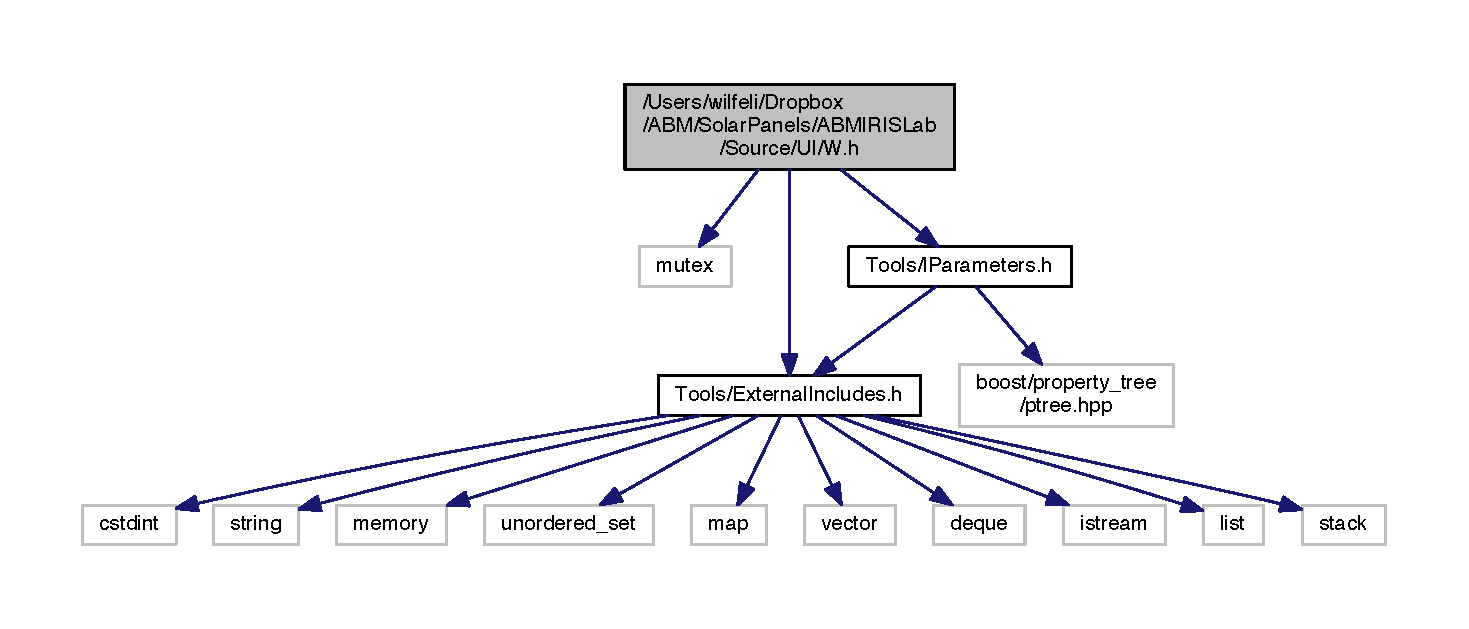
\includegraphics[width=350pt]{_w_8h__incl}
\end{center}
\end{figure}
This graph shows which files directly or indirectly include this file\+:
\nopagebreak
\begin{figure}[H]
\begin{center}
\leavevmode
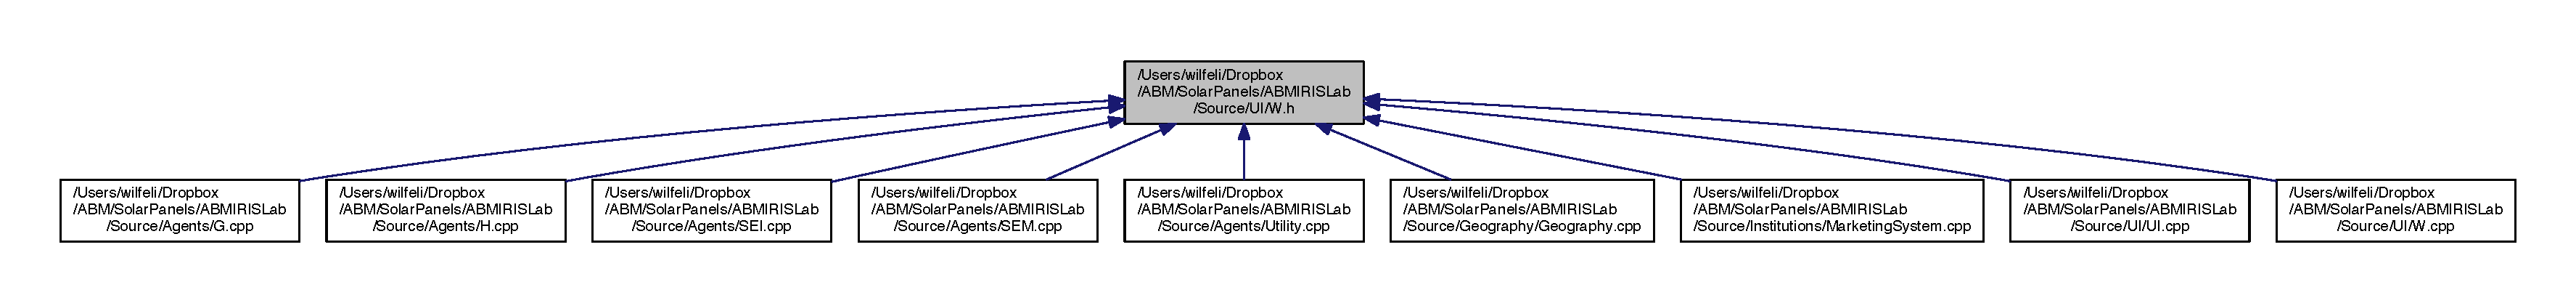
\includegraphics[width=350pt]{_w_8h__dep__incl}
\end{center}
\end{figure}
\subsection*{Classes}
\begin{DoxyCompactItemize}
\item 
class \hyperlink{classsolar__core_1_1_w}{solar\+\_\+core\+::\+W}
\end{DoxyCompactItemize}
\subsection*{Namespaces}
\begin{DoxyCompactItemize}
\item 
 \hyperlink{namespacesolar__ui}{solar\+\_\+ui}
\item 
 \hyperlink{namespacesolar__core}{solar\+\_\+core}
\end{DoxyCompactItemize}

%--- End generated contents ---

% Index
\backmatter
\newpage
\phantomsection
\clearemptydoublepage
\addcontentsline{toc}{chapter}{Index}
\printindex

\end{document}
